%   DOCUMENT CLASS  %%%%%%%%%%%%%%%%%%%%%%%%%%%%%%%%%%%%%%%%%%%%%%%%%%%%%%%%%%%
%
%   Use the `sfuthesis` class to format your thesis.
%
%   For more information about thesis formatting requirements, go to
%   http://www.lib.sfu.ca/help/publish/thesis or ask a thesis advisor at the
%   SFU Research Commons.


\documentclass{sfuthesis}



%   DOCUMENT METADATA  %%%%%%%%%%%%%%%%%%%%%%%%%%%%%%%%%%%%%%%%%%%%%%%%%%%%%%%%
%
%   Fill in the following information for the title page and declaration of
%   committee page. Please review the Declaration of Committee page
%   instructions on the library's thesis website before completing this page:
%   https://www.lib.sfu.ca/help/publish/thesis/format/declaration-committee

%   Choose the \faculty entry below from the following list:
%
%       - Faculty of Applied Sciences
%       - Faculty of Arts and Social Sciences
%       - Beedie School of Business
%       - Faculty of Communication, Art and Technology
%       - Faculty of Education
%       - Faculty of Environment
%       - Faculty of Health Sciences
%       - Faculty of Science
%       - Faculty of Graduate Studies
%       - School of Medicine


\title{Human-Centric Design for Data-Driven Decision Support}
\thesistype{Thesis}
\author{Mehdi Vahabisani}
\previousdegrees{%
    M.Sc., Tarbiat Modares University, 2022\\
    B.Sc., University of Tehran, 2019}
\degree{Masters of Science}
\department{School of Interactive Arts and Technology}
\faculty{Faculty of Communication, Art and Technology}
\copyrightyear{2026}
\semester{Summer 2026}


%   You may include up to six keywords or phrases. Keywords should be separated
%   with semicolons. No punctuation at the end.
\keywords{Data-Driven Decision-Making; Decision Support Systems; Human-Centered Design; Causal Reasoning; Visual Analytics; Decision Intelligence}

\committee{
    \chair{Kate Hennessy}{Associate Professor, School of Interactive Arts and Technology}
    \member{Brian Fisher}{Supervisor \\ Professor, School of Interactive Arts and Technology}
    \member{Wolfgang Stuerzlinger}{Committee Member \\ Professor, School of Interactive Arts and Technology}
}


%   PACKAGES %%%%%%%%%%%%%%%%%%%%%%%%%%%%%%%%%%%%%%%%%%%%%%%%%%%%%%%%%%%%%%%%%%
%
%   Add any packages you need for your thesis here.
%   You don't need to call the following packages, which are already called in
%   the sfuthesis class file:
%
%   - appendix
%   - etoolbox
%   - fontenc
%   - geometry
%   - lmodern
%   - nowidow
%   - setspace
%   - tocloft
%
%   If you call one of the above packages (or one of their dependencies) with
%   options, you may get a "Option clash" LaTeX error. If you get this error,
%   you can fix it by removing your copy of \usepackage and passing the options
%   you need by adding
%
%       \PassOptionsToPackage{<options>}{<package>}
%
%   before \documentclass{sfuthesis}.
%
%   The following packages are a few suggestions you might find useful.
%
%   (1) amsmath and amssymb are essential if you have math in your thesis;
%       they provide useful commands like ``blackboard bold'' symbols and
%       environments for aligning equations.
%   (2) amsthm includes allows you to easily change the style and numbering of
%       theorems. It also provides an environment for proofs.
%   (3) graphicx allows you to add images with \includegraphics{filename}.
%   (4) pdfx is required to create a PDF/A version of your thesis file.
%   (5) hyperref turns your citations and cross-references into clickable
%       links, and adds metadata to the compiled PDF. Don't add options to the hyperref package as 
%	these will conflict with the pdfx package. 
%   (6) pdfpages lets you import pages of external PDFs using the command
%       \includepdf{filename}. You will need to do this if your research
%       requires an Ethics Statement, so uncomment that line below. 
%

\usepackage{amsmath}                            
\usepackage{amssymb}                            
\usepackage{amsthm}                             
\usepackage{graphicx}       
% The pdfx package is needed here to make a PDF/A version of your thesis. Don't change the order in which the following two lines appear, and don't add any options to the hyperref package.           
\usepackage[a-1b]{pdfx}      
\usepackage{hyperref}    
\usepackage{longtable}
\usepackage{booktabs}
\usepackage{multirow}
\usepackage{array}
\usepackage{pdflscape}
\usepackage{multicol}
\usepackage{array}
\usepackage{ragged2e}
\usepackage{fancyhdr}
\usepackage{adjustbox}
\usepackage{tabularx}
\fancypagestyle{landscape-page}{%
    \fancyhf{} % clear all headers and footers
    \fancyfoot[C]{\thepage} % force page number to bottom center
    \renewcommand{\headrulewidth}{0pt} % remove header rule if desired
}          
%\usepackage[pdfborder={0 0 0}]{hyperref}        
% \usepackage{pdfpages}                         
% ...
% ...
% ...
% ... add your own packages here!




%   OTHER CUSTOMIZATIONS %%%%%%%%%%%%%%%%%%%%%%%%%%%%%%%%%%%%%%%%%%%%%%%%%%%%%%
%
%   Add any packages you need for your thesis here. We've started you off with
%   a few suggestions.
%
%   (1) Use a single word space between sentences. If you disable this, you
%       will have to manually control spacing around abbreviations.
%   (2) Correct the capitalization of "Chapter" and "Section" if you use the
%       \autoref macro from the `hyperref` package.
%   (3) The LaTeX thesis template defaults to one-and-a-half line spacing. If
%       your supervisor prefers double-spacing, you can redefine the
%       \defaultspacing command.
%

\frenchspacing                                    % (1)
\renewcommand*{\chapterautorefname}{Chapter}      % (2)
\renewcommand*{\sectionautorefname}{Section}      % (2)
\renewcommand*{\subsectionautorefname}{Section}   % (2)
% \renewcommand{\defaultspacing}{\doublespacing}  % (3)
% ...
% ...
% ...
% ... add your own customizations here!




%   FRONTMATTER  %%%%%%%%%%%%%%%%%%%%%%%%%%%%%%%%%%%%%%%%%%%%%%%%%%%%%%%%%%%%%%
%
%   Title page, committee page, abstract, dedication, acknowledgements, table
%   of contents, etc.
%
%   If your research requires an Ethics Statement, download the pdf from
%   https://www.lib.sfu.ca/help/publish/thesis/regulations#ethics-statement
%   to your thesis folder, then uncomment the appropriate lines below.

\begin{document}

\frontmatter
\maketitle{}
\makecommittee{}

%\addtoToC{Ethics Statement}%
%\includepdf[pagecommand={\thispagestyle{plain}}]{ethics_statement_piii.pdf}%
%\clearpage

\begin{abstract}
Organizations increasingly employ data-driven technologies to support decision-making; however, existing approaches remain fragmented and often overlook decision-makers’ causal reasoning, cognitive characteristics, and task requirements. This thesis investigates how diverse data-driven techniques can be systematically integrated to enhance organizational decision-making. Through thematic and textual analyses of literature on data-driven decision making, causal reasoning, and human-centered decision support, six major classes of data-driven techniques are identified, and their roles across decision-making stages are examined. The findings are synthesized into a human- and task-centered framework that orchestrates visualization, machine learning, traditional statistical analysis, natural language models, mathematical optimization, and simulation across different stages of decision-making, providing the foundation for practical integration of these diverse tools according to decision tasks, causal knowledge, and cognitive capacities. Building upon this framework, the thesis proposes a conceptual decision support system architecture that demonstrates how these technologies can be effectively combined in practice to improve decision quality, efficiency, transparency, and decision-makers’ confidence in complex organizational environments.
\end{abstract}


\begin{dedication}
This is an optional page. Use your choice of paragraph style for text on this page.
\end{dedication}


\begin{acknowledgements}
This is an optional page. Use your choice of paragraph style for text on this page.
\end{acknowledgements}

\addtoToC{Table of Contents}%
\tableofcontents%
\clearpage

%   This is an optional page. Remove the following lines if you don't have any tables.
\addtoToC{List of Tables}%
\listoftables%
\clearpage

%   This is an optional page. Remove the following lines if you don't have any figures.
\addtoToC{List of Figures}%
\listoffigures%
\clearpage





%   MAIN MATTER  %%%%%%%%%%%%%%%%%%%%%%%%%%%%%%%%%%%%%%%%%%%%%%%%%%%%%%%%%%%%%%
%
%   Start writing your thesis --- or start \include ing chapters --- here.
%

\mainmatter

\chapter{Introduction}
\section{Background and Importance}
In everyday life, we humans face situations in which we need to select one option from multiple possibilities to satisfy our goals. To get to work, we might think of either taking public transit to minimize transportation costs and environmental damage or using a personal vehicle to minimize travel time and achieve comfort. Among several possible trip destinations, we weigh all options according to their cost, people’s ratings, perceived beauty of places and natural sights, etc., and pick the one that is predicted to cause the highest satisfaction. The list can, of course, go on and include tons of these routine decisions. Inside businesses and governmental organizations, decision-making is also one of the most common activities of managers across various levels of the organization’s hierarchy. At the departmental level, a manager of a department like Sales in an organization may have to decide on either spending their limited advertisement budget to acquire new customers or focusing on upselling to their current customers. The chief executive officer of the same company, however, may need to make a decision on which continents or countries they should expand their business into to gain a higher market share. While the impact for each of these decision’s outcome is variable depending on the decision’s nature and the organizational level the decision is being made in, the decision-making individuals of any organizational level share roughly similar forms of activities that involve generating decision alternatives, predicting the outcome(s) for each generated alternative, weighing alternatives based on their predicted outcome, and selecting the one that corresponds to the most satisfactory outcome. For the sake of organizational prosperity, not only should the efficiency and quality of the predictions for the outcome of the decision be taken care of, but the confidence of decision-makers in the quality of the decision made should also be improved. The results of a survey suggest that the majority of organizational executive managers spend more than one-third of their time on making decisions, in which half of this time is used “ineffectively”, resulting in an estimated 250 million dollars salary cost ~\cite{smet_three_nodate}. Not only being time-inefficient, but also the organizational decision-makers in these studies have self-reported the quality of their decision outcomes as poor in general ~\cite{smet_three_nodate}. One of the most highly reported reasons for this widespread dissatisfaction is the lack of clear decision-making practices to deal with the complexities of decision-making in a co-evolving business environment ~\cite{smet_three_nodate}. These complexities often arise as the number of intervening decision variables increases, making both the prediction and comparison of the outcomes upon selecting each decision alternative difficult. Current decision-making research has become highly fragmented between disciplines and specialized perspectives (e.g., operational research, psychology, and management), with little progress towards an integrated understanding of the overall decision-making process in which the role of the above-mentioned complexities is highlighted ~\cite{adinolfi2021journey}. Furthermore, the quality of decision-making in such complex environments improves when the decision-maker has a more accurate judgment about the relationships between the variables of the decision problem ~\cite{janssen2017factors}. Many organizations these days use technologies based on data sources to gain more powerful insights into different aspects of their business, from the operational level up to the strategic level. However, the insufficiency of practices that align the application of these data-driven tools with the actual decision problems and the decision-makers' knowledge about the problems has hampered organizations from benefiting from the full potential of such tools. The existing literature on decision support frameworks is mainly populated by those publications in which the emphasis has been heavily placed on the value that data-driven tools bring for decision-makers, while the role of decision-makers’ intuitive reasoning, domain knowledge, and interpersonal traits in exploiting the analytical outputs of these tools has been generally neglected ~\cite{janssen2017factors}. Therefore, more investigation into the mediating effect of decision-makers’ intuition and cognitive characteristics on the extent of benefit they might receive from data analytics tools is needed.
\section{Research Goal and Questions}
In this Master of Science thesis, we aim to introduce both a conceptual framework and a decision support system (DSS) architecture that articulate an integrated application of data-driven tools to conform to decision task requirements as well as decision-makers’ causal knowledge and cognitive capacities in identifying, analyzing, and solving organizational decision-making problems. To achieve this, we first need to identify the most common data-driven tools and techniques that have been used in previous research publications to aid decision-makers in performing decision-making activities. Then we shed light on each of these techniques’ strengths, weaknesses, and intended use cases when it comes to utilizing them in an organizational decision problem. Answering the following research questions (RQs) will aid us in scaffolding a solid foundation for such a multi-dimensional and integrative framework:\par
RQ1: What are the most common data-driven tools and techniques that are used to assist decision-makers in organizations?\par
RQ2: How do these data-driven tools augment organizational decision processes? \par
RQ3: What is the role of human causal reasoning in decision-making? How can it be used in alignment with data-driven tools to augment organizational decisions?\par
RQ4: What could a data-driven decision-making process that also leverages human causal knowledge and their cognitive abilities look like? How might we design it in practice?\par
In the following section of the current chapter, we provide the outline of the overall research methodology that helps us find the answers to the above RQs. The answers to the first two RQs are derived from reviewing data-driven decision-making literature that is conducted in the 2\textsuperscript{nd} chapter, while the review and analysis of existing literature on the role of causal reasoning, cognitive capacities, and other influential personal characteristics in decision-making in the 3\textsuperscript{rd} chapter direct us to find RQ3’s answer. We then exploit the information in our collected research evidence to design the framework at the conceptual level in the 4\textsuperscript{th} chapter as the answer to RQ4. In the 5\textsuperscript{th} chapter, the practical design of a decision-support system implementing the most important functional aspects of the proposed framework is presented with the aid of technical documentation and UI prototypes as proof-of-concept. Finally, in the 6t\textsuperscript{th} chapter, we derive conclusions from all the discussions that were made in previous chapters, and delineate the road plan for future studies.
\section{Methodology and Research Methods}
We expressed our goal for this research to be the proposition of a decision support design process framework and system architecture that seeks to maximize the value of data-driven tools in the decision-making process by aligning their design and application with decision-makers’ cognitive capacities, domain knowledge, and intuitive reasoning of causal relations. To be able to enhance the extent of profit that is achieved by the data science techniques and tools, we need to identify the most frequently used classes of data-driven tools/techniques first (which is the answer to RQ1), and uncover the ways that these tools assist decision-makers, along with their limitations and challenges (which is the answer to RQ2). Aiming to address these challenges by incorporating decision-maker(s) causal knowledge of the problem domain, we explore the role of causal reasoning in decision-making tasks and how it can constructively frame and specify the data and data-driven tools that are either necessary or useful for making an informed decision (the answer to RQ3). Based on the information we receive from exploring these studies, we will then brainstorm how to design different pieces of the integrative framework, leveraging both data-driven tools and decision-makers’ causal knowledge and characteristics (as the answer to RQ4), which precedes the architecture of a decision-support system that implements the framework for assisting decision-making users in real-world decision problems. Figure \ref{ResearchProcess} demonstrates the process flowchart for the research methodology that we have designed for the current thesis. According to Figure \ref{ResearchProcess}, each of the expressed RQs at the end of the first chapter is answered in our work by employing one or two of the research methods (connected with dashed-line arrows) in the figure’s left lane. The answer to each RQ is one or multiple pieces of information output in the form of narrative textual summaries or graphical models of the integrative framework and the system architecture. The information outputs (as the answers to RQs) can in turn be used to answer the subsequent RQs (visualized by solid-line arrows).\par
\begin{figure}
    \centering
    % Ensure figure width fits within SFU margins
    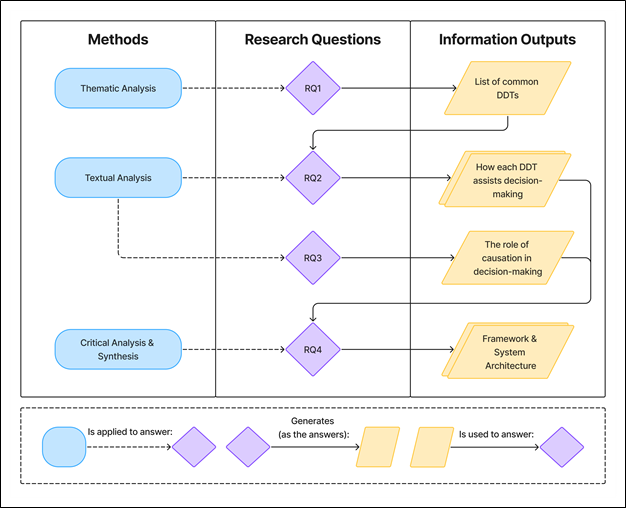
\includegraphics[width=6in]{Figures/ResearchProcess.png} % ≤ 6 inches wide
    \caption[Research process workflow]{The research's flow of information, activities, and methods used to answer our research questions (RQs)}
    \label{ResearchProcess}
\end{figure}
It is now inferred that the development of the framework is dependent on finding the answer to each of the RQs from 1 to 3. We employ different methods to answer each of these RQs based on the nature of the question. The answer to RQ1—a list of tools/techniques that have been frequently mentioned and used in the literature for decision assistance—is found by the identification and re-labeling of recurring themes (thematic analysis) inside the existing literature for data-driven decision-making (DDDM). To understand how those data-driven tools that were found in the first step currently improve decision-making processes (the answer to RQ2), a narrative that is based on textual analysis of the literature is produced for each tool or technique. The imperative role of human causal reasoning in decision-making as the answer to RQ3 is similarly derived from a textual analysis of the publications on the relationship between decision-making and causality. The combination of the answers to the last three questions will direct us to find the answer to RQ4, for which we employ a critical approach to address the current challenges in the use of data-driven tools for decision augmentation from a human-and-task-centered standpoint. 

\chapter{Literature I: Data-Driven Decision-Making}
\section{Decision Theory}
Inside the realm of various fields of human sciences, such as philosophy, economics, business and commerce, and more recently, behavioral and cognitive psychology, decision-making has been largely investigated as one of the most remarkable activities of humans, or perhaps, some other intelligent organisms and systems. In ancient Greek philosophy, Aristotle introduced the notion of “phronesis” as a human intellectual virtue that enables him to make rational, sound judgments, realizing his “practical wisdom”~\cite{bartlett_aristotles_2011}. In early modern philosophy, Descartes (1596-1650) was the one who placed an emphasis on human intellect to derive knowledge, rational conclusions, and sound judgments out of sensory information, utilizing critical reasoning and “methodological doubt”~\cite{descartes_meditations_2008}. In contrast to rationalist philosophers such as Descartes, empiricists such as David Hume (1711-1776) viewed human reasoning as a “slave” of his passions, resulting in judgments being derived by sentiments such as love, hate, and fear; thus, human actions upon these judgments are inherently gestures of approval or disapproval, rather than objective behaviors~\cite{hume_treatise_2000}. Finally, Immanuel Kant (1724-1804) synthesizes these two different views utilizing an analogy between “theoretical reason” and “practical reason”. According to Kant’s philosophy, theoretical reasoning is the type of reasoning that aims to understand the universal laws about the natural world that are in the form of truth, knowledge, and causal principles, while practical reasoning is to understand what ought to be done within a set of choices bounded by moral obligations. The former reasoning is ultimately used towards constitutive judgment that defines objects’ essence or structure of experiences, and the latter facilitates “regulative judgment” that normatively guides and directs human actions and defines their moral behaviors~\cite{de_pierris_kant_2008}.\par
Contemporary philosophical views on human reasoning and decision-making are mainly influenced by the dawn of theories in modern psychology and economics, as well as the advances in computational logic~\cite{steele_decision_2020}. The normative accounts of decision theories highlight the role of rationality in the reasoning behind decision-making agents’ choices. Decision theory constitutes the foundational body of knowledge concerned with how decisions ought to be made (normative accounts), how decisions are made in practice (descriptive accounts), and how decision processes can be improved through structured interventions and tools (prescriptive accounts). These perspectives jointly inform contemporary research on organizational decision-making and the design of data-driven decision support systems.
\subsection{Normative Decision Theory and Expected Utility}
In 1947, John von Neumann (1903-1957) and Oskar Morgenstern (1902-1977) introduced one of the most famous theories on rational decision-making, which was called the \textbf{expected utility theorem (EUT)}. In their mutual book "Theory of Games and Economic Behavior", they developed a probabilistic model to mathematically represent how a rational agent might prefer an option (also called a \textit{prospect}) over others in a lottery by seeking the alternative that maximizes the expected value of a utility function weighted by subjective probabilities of outcomes. Under EUT, rational preferences must satisfy a set of axioms such as completeness, transitivity, and independence.\par
Although EUT provides a mathematically coherent benchmark for rational choice, extensive empirical research has demonstrated systematic violations of its axioms in real human decision behavior. Behavioral experiments show that individuals often exhibit inconsistent preferences, probability misjudgments, and context-dependent evaluations, particularly in complex or uncertain environments~\cite{edwards_behavioral_1961, briggs_normative_2014}. These findings suggest that purely normative models, while analytically powerful, are insufficient for explaining or supporting real-world organizational decisions.
\subsection{Descriptive Decision Theory and Behavioral Deviations}
In response to the descriptive inadequacy of EUT, behavioral decision theory emerged to empirically investigate how humans actually make judgments and choices. Most notably framed by Tversky and Kahneman~\cite{tversky1978judgment}, this stream of research demonstrates that decision-makers rely on heuristics—cognitive shortcuts that reduce computational effort but may introduce systematic biases. Such biases include loss aversion, framing effects, and probability weighting, all of which challenge the assumptions of perfect rationality embedded in normative models~\cite{einhorn1981behavioral,frisch_beyond_1994}. Prospect theory and related models further illustrate that decision-makers evaluate outcomes relative to reference points and are disproportionately sensitive to losses compared to gains. These descriptive insights are particularly relevant for organizational contexts, where decisions often involve uncertainty, competing objectives, and high cognitive load.
\subsection{Bounded Rationality and Cognitive Constraints}
A pivotal bridge between normative ideals and descriptive realities is the concept of \textbf{bounded rationality}, originally proposed by Herbert Simon~\cite{simon1972theories}. Bounded rationality posits that human decision-makers operate under constraints of limited information, limited time, and limited cognitive processing capacity. Rather than optimizing, individuals often \textit{satisfice}—seeking solutions that are “good enough” given these constraints~\cite{jones_bounded_1999,gigerenzer_what_2020}.\par
From this perspective, deviations from expected utility maximization are not irrational failures, but adaptive responses to environmental and cognitive limitations. Subsequent work has formalized bounded rationality into alternative decision models that retain probabilistic reasoning while relaxing strict rationality assumptions~\cite{navarro-martinez_boundedly_2018,katsikopoulos_one-reason_2008}.
\subsection{Prescriptive Decision Theory and Decision Support}
Prescriptive decision theory focuses on improving decision outcomes by designing methods, representations, and tools that compensate for human cognitive limitations while preserving human judgment and domain expertise. This orientation is particularly relevant to \textbf{data-driven decision-making (DDDM)}, where analytical models and computational tools are introduced to augment—rather than replace—human decision-makers.\par
From a prescriptive standpoint, decision support systems should not merely compute optimal solutions but should structure information, reveal trade-offs, and support sense-making in ways that align with human cognitive capacities. This insight directly motivates the integration of data-driven tools with human-centric design principles, such as transparency, interpretability, and cognitive fit. Rather than enforcing a single notion of optimality, prescriptive approaches emphasize decision quality, confidence, and usability within realistic organizational constraints.
\subsection{Implications for Human-Centric DDDM}
Taken together, these theoretical developments suggest that effective decision support frameworks must balance formal rationality with behavioral realism. Normative models provide clarity and structure, behavioral theories reveal systematic human tendencies and limitations, and bounded rationality explains why decision support tools are necessary in the first place. Consequently, data-driven decision-making frameworks should be designed to externalize complex computations, reduce cognitive load, and support causal reasoning, while allowing decision-makers to apply their intuition and contextual knowledge. This synthesis of decision theory establishes the conceptual foundation for the subsequent sections of this thesis, which investigate how data-driven tools and human causal reasoning can be orchestrated across different stages of the organizational decision process.

\section{DDDM Background}
The advances in information technology and web-based communication have made access to various sources of information and data easier and more efficient than ever~\cite{provost_data_2013}. The majority of organizations now log and store the data from their operational transactions inside data repositories to act upon them later in other activities, or to derive analytical insights for process improvement and planning. The analytical purposes for collecting and storing data include, but are not necessarily limited to, decision-making. DDDM is, in fact, the concept and the practice of basing decisions on the analysis derived from data, in order to set boundaries for DMs’ over-reliance on their pure intuition and to shed light on their faulty mental assumptions and unnoticed aspects in a decision problem. As the raw data is not directly usable for deriving analytics from, additional actions are required to transform the raw data into useful information and knowledge that can help DMs recognize, structure, and solve decision problems. Thus, apart from the collection and storage of data, DDDM involves data cleaning, re-organization, analysis, summarization, synthesis, and prioritization~\cite{mandinach_theoretical_2006}. At the practical level, DDDM is observed to be realized by the application of algorithm-based and data mining systems that recognize hidden patterns in the accessible data~\cite{provost_data_2013}. Figure \ref{DDDMProcess} demonstrates the conceptual model of the DDDM process presented by Mandinach et al.~\cite{mandinach_theoretical_2006}. According to them, technology-based tools are mainly applied to the data and information processing layers of the DDDM process to facilitate the collection, organization, analysis, and summarization of data and extracted information.\par
\begin{figure}
    \centering
    % Ensure figure width fits within SFU margins
    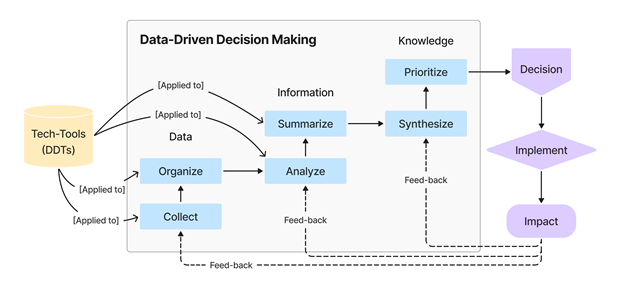
\includegraphics[width=6in]{Figures/DDDMProcess.png} % ≤ 6 inches wide
    \caption[DDDM conceptual process model]{Conceptual process model of data-driven decision-making (adopted and re-built from Mandinach et al.~\cite{mandinach_theoretical_2006})}
    \label{DDDMProcess}
\end{figure}
Despite the growing adoption of data-driven decision-making practices across organizational contexts, the literature consistently reports a set of limitations that hinder the full realization of DDDM’s promised benefits. One of the most frequently cited challenges is the \textbf{over-reliance on algorithmic outputs without sufficient contextual interpretation}, which may lead to misguided decisions when the underlying assumptions of analytical models do not align with the real-world decision environment~\cite{power_decision_2008}. While advanced analytics can uncover statistical regularities and correlations in data, they often fail to provide actionable explanations regarding \textit{why} certain patterns emerge, limiting their usefulness in complex or novel decision scenarios.\par
Another critical challenge pertains to \textbf{data quality and relevance}. Data-driven tools are inherently dependent on the availability, accuracy, and representativeness of input data. In organizational settings, data is frequently incomplete, biased, or collected for purposes other than decision support, resulting in analytical outputs that may be misleading or difficult to interpret~\cite{sarker_data_2021}. Moreover, the increasing volume and dimensionality of data can overwhelm decision-makers, exacerbating cognitive overload rather than alleviating it.\par
From a human-centered perspective, DDDM systems often suffer from \textbf{limited transparency and interpretability}, particularly when complex machine learning models or automated optimization techniques are employed. Black-box models may produce accurate predictions, yet their internal logic remains inaccessible to decision-makers, undermining trust and reducing users’ willingness to rely on analytical recommendations~\cite{bubeck_sparks_2023}. This lack of explainability is especially problematic in high-stakes organizational decisions, where accountability and justification are essential.
\subsection{Organizational and Cognitive Barriers to Effective Implementation of DDDM}
Beyond technical limitations, organizational and cognitive factors play a significant role in shaping the effectiveness of data-driven decision-making. Prior studies emphasize that organizations vary substantially in their\textbf{ absorptive capacity}—that is, their ability to recognize the value of data-driven insights, assimilate analytical knowledge, and apply it effectively in decision processes~\cite{mba_in_management_lamar_university_usa_impact_2025}. Even when advanced decision support systems are available, decision-makers may lack the necessary analytical literacy or domain-specific understanding to interpret results appropriately.\par
Cognitively, human decision-makers are constrained by limited working memory, attentional resources, and reasoning capacity. As a result, presenting large volumes of analytical output without proper structuring or prioritization can impede sense-making and reduce decision confidence. Empirical evidence suggests that decision-makers often struggle to integrate quantitative outputs with their existing mental models and domain knowledge, leading either to blind acceptance or outright rejection of analytical recommendations~\cite{rahman_data-driven_2021}.\par
These challenges highlight a fundamental tension in DDDM research: while data-driven tools excel at computation, pattern recognition, and optimization, \textbf{decision-making remains an inherently human activity} that involves judgment, causal reasoning, and contextual understanding.
\subsection{Toward Human-Centric Data-Driven Decision Support}
The limitations identified in the DDDM literature indicate that effective decision support cannot be achieved solely through increased automation or analytical sophistication. Instead, contemporary research increasingly advocates for \textbf{human-centric data-driven decision support systems} that explicitly account for decision-makers’ cognitive processes, domain expertise, and reasoning strategies~\cite{brandas_data_2016,hayn_predictive_2018}.\par
Such systems aim not only to deliver predictions or optimal solutions but also to facilitate \textbf{sense-making, exploration, and explanation} throughout the decision process. Rather than replacing human judgment, data-driven tools are positioned as cognitive partners that externalize complex computations, surface relevant information, and support the evaluation of trade-offs among competing decision criteria. This perspective aligns closely with prescriptive decision theory and bounded rationality, emphasizing the role of tools in compensating for human cognitive limitations while preserving human agency.\par
Importantly, recent advances in analytics—such as interactive visualization, simulation, and explainable machine learning—offer new opportunities to align computational outputs with human causal reasoning. By enabling decision-makers to explore hypothetical scenarios, inspect relationships among variables, and iteratively refine assumptions, these tools can bridge the gap between statistical analysis and practical decision-making.
\subsection{Implications for the Present Research}
The reviewed DDDM literature demonstrates that while data-driven tools provide powerful mechanisms for analyzing complex organizational environments, their effectiveness is contingent upon how well they are integrated into the broader decision-making process. The absence of explicit alignment between analytical tools and human reasoning remains a key gap in existing frameworks.\par
This observation directly motivates the present research, which seeks to design an \textbf{integrated data-driven decision-making framework} that systematically orchestrates data-driven tools across different decision stages while accounting for decision-makers’ cognitive characteristics and causal understanding. In the following chapters, we build upon these insights to explore how causal reasoning and human-centric design principles can be combined with data-driven techniques to enhance decision quality, confidence, and efficiency in organizational contexts.

\section{Data-Driven Decision-Making Tools and Techniques}
The very first step towards facilitating and tailoring data-driven tools for organizational decision processes is to identify the tools and techniques at the abstract level that have been employed for extracting actionable insights in decision-making research literature. In this section, we dig into the content of those research publications that incorporate the use of data analysis in different forms to support decisions in various domains. Then, we classify the recurring themes of methods, tools, and techniques into abstract thematic codes. As our goal here is to understand what types of data-driven tools have been mainly employed to assist decision-makers, we only consider the publications with a practical approach towards designing and building data-driven decision support systems (DSSs) in a domain such as education.
\subsection{Search Process}
We began the process by providing the following prompt to Web of Science (WoS) and PubMed\footnote{The results of the search were filtered to those publications with “Abstract” and “Full text” availability in the PubMed directory.} databases:\par
\begin{center}
\textit{“data-driven”} AND (\textit{“decision-making”} OR \textit{“Decision-support System”})
\end{center}
As expected, the number of results that include the keywords in either the title or abstract is too much; therefore, we only consider the top 100 search results in both directories and select those that have a practical approach, judging primarily based on their abstract, methodology, and conclusion sections. For example, a paper with the title “\textit{An adaptive decision support system for outpatient appointment scheduling with heterogeneous service times}”~\cite{feng2024adaptive} is included because of its practical and domain-oriented approach, while the one with the title “\textit{A Conceptual Framework for Data-Driven Decision Making}”~\cite{gill_conceptual_2014} is disregarded as we found no implications of implementing data-driven tools towards DDDM in different sections of the paper’s full-text.
\subsection{Search Result and Observed Themes}
Upon carefully reviewing the resulting publications’ abstract, methodology, and conclusion sections, we identified 72 publications that were relevant to our purpose and had a direct reference to a specific data analysis method (e.g., \textit{regression}); of which 34 were from WoS and 38 from PubMed. All of these studies have been published in or after 2010, with 55 (76\%) of them published in or after 2020. The specific data analysis methods (for decision-making purposes), mathematical models of decision-making, and developed end-user tools to assist decision-makers were coded in all these studies. Many of these codes (e.g., \textit{dashboard}) were consistently repeated over several other publications in our selected set, resulting in a collection of 49 coded methods that were later classified into intermediate and final themes as reported in Table \ref{A1:DDTSurvey}.\par
We observed in 10 publications that conventional \textbf{supervised machine learning (SML)} techniques, such as \textit{linear regressions (LR), logistic regression, support vector machine (SVM), k-nearest neighbors (KNN),} and \textit{decision tree} algorithms, have been applied to structured and labeled datasets for prediction and classification purposes to support decision-making. In 4 publications, we also witnessed the adoption of ad hoc SML algorithms to perform classification tasks in support of a decision-making problem. Ensemble ML techniques (e.g., \textit{random forest, gradient boosting}) have also been employed to realize SML for both prediction and classification in 8 papers. Rule-based methods have also been used in 2 publications for classification tasks. \textbf{Unsupervised machine learning (USML)} techniques have also been used for clustering tasks as part of decision-making processes in 7 papers. Being involved in 3 papers, the application of \textit{k-means} was found to be prevalent in the studies utilizing USML. \textbf{Reinforcement learning (RL)}, as the third category of ML algorithms, was seen to be employed in 3 publications as well. Additionally, 8 publications have employed different variations of \textit{neural network (NN)} models (e.g., \textit{deep neural networks}) to realize supervised or unsupervised learning for prediction, classification, dimensionality reduction, and clustering purposes.\par  
Other than the above AI-related statistics-based techniques, we have also identified 6 studies making use of statistical methods in the form of inferential statistics and time-series analysis methods (e.g., \textit{ARIMA}). We subsequently categorized these methods into the final theme of \textbf{traditional statistics (TS)} to distinguish them from the previously mentioned ML models, which are also statistics-based.\par
Unlike the statistics-based methods that operate on structured datasets to derive information, \textit{natural language processing (NLP)} techniques, as another branch of AI tools, are capable of processing unstructured data (e.g., text or audio) to derive meanings and information from the source and/or to generate human-language responses to user prompts. 3 studies in our selected set have either developed NLP models for their specific cases or utilized an existing off-the-shelf \textit{large language model (LLM)} for human language processing. Despite the fact that these models extensively incorporate deep neural networks and ML models themselves, we still classify them into a separate theme of \textbf{language models (LMs)}.\par 
Another one of the frequently emerging classes of data-driven techniques that has helped DDDM to be accomplished is \textbf{data visualization (VIZ)}. In 22 papers, the design and development of a group of visual interfaces (i.e., \textit{dashboards}) to help decision-makers access a broad set of information in a visual form—that is more affordable to the human cognitive system—is involved. The application of a single chart type (e.g., \textit{line charts}) in DSS interfaces was only observed in 11 studies. In addition, 3 studies have utilized node-link visual models (e.g., \textit{causal networks}) to better illustrate intricate relationships between decision variables.\par
We also found 18 studies that incorporate mathematical decision-making models and algorithms to discover an optimal choice from a discrete or continuous set of decision alternatives. \textit{Single-objective} and \textit{multi-objective}/\textit{multi-criteria} mathematical models have both been developed in such studies for decision optimization. These models were either heuristically created or selected from the conventional models, like the \textit{analytic hierarchy process (AHP)}, to calculate the utility values of the alternatives, leading to the specification of the optimal solution or alternative. We therefore classify all of these codes into a grander theme of \textbf{mathematical optimization (MO)}, involving any method or algorithm that formally discovers a single or a set of optimal solutions to a decision-making problem.\par
Last but not least, 9 studies have employed different classes of simulation methods to either test and virtually imagine the outcomes of taking any hypothetical set of actions towards solving a decision problem, or estimate the missing values of some variables of interest in the context of a decision problem. Stochastic simulation methods (e.g., \textit{Monte-Carlo simulation}), structural equation-based methods (e.g., \textit{system dynamics simulation}), agent-based simulation, and self-learning data-driven simulation methods were the types of simulations seen in these studies. We categorize these codes into the \textbf{simulation (SIM)} theme.
Figure ~\ref{DDDMSearchProcess} summarizes the information on the entire search process and the intermediate and final classified themes as a result of the thematic analysis performed on the DDDM literature.\par
\begin{figure}
    \centering
    % Ensure figure width fits within SFU margins
    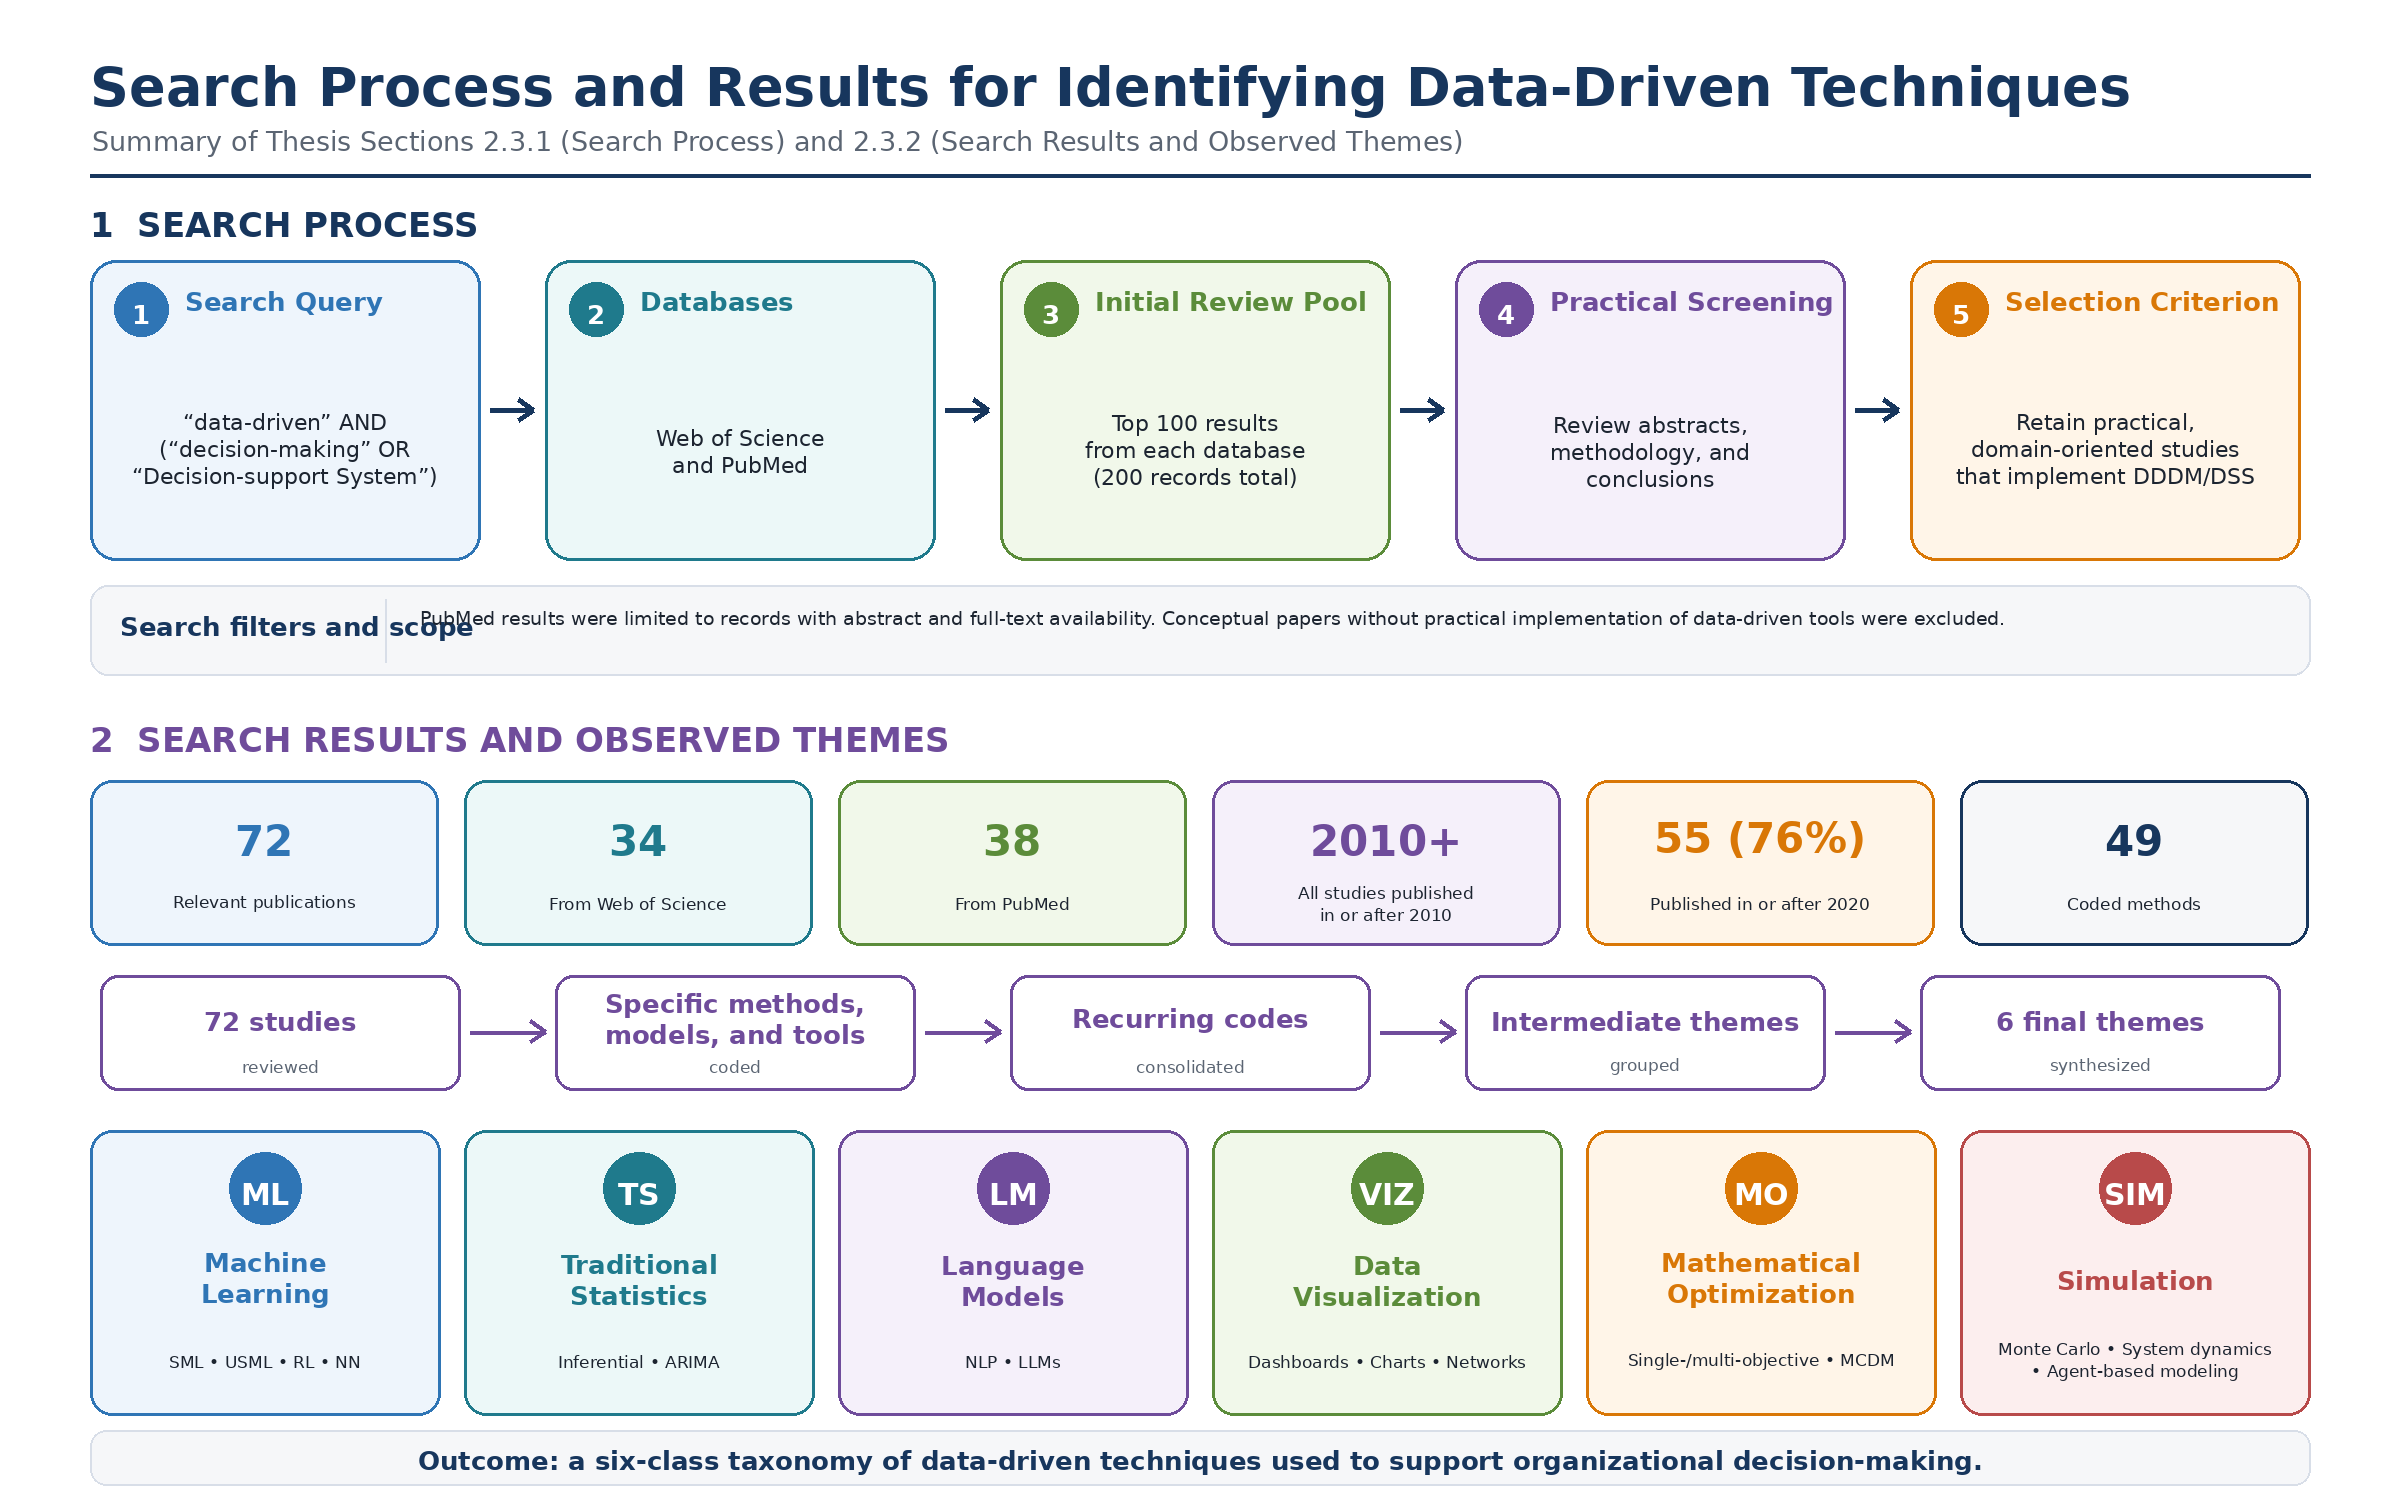
\includegraphics[width=6in]{Figures/DDDMLitReview_search_summary.png} % ≤ 6 inches wide
    \caption[DDDM literature search process and resulting themes]{Search process and results of the thematic analysis for identification of data-driven techniques (DDTs) from data-driven decision-making (DDDM) literature (Generated by Gen-AI)}
    \label{DDDMSearchProcess}
\end{figure}
\subsection{Summary of Observed Classes of Data-Driven Techniques that Assist Decision-Making (Answer to RQ1)}
According to the results of the performed thematic analysis, we answer our first research question “\textit{\textbf{RQ1: What are the most common data-driven tools and techniques that are used to assist decision-makers in organizations?}}" as a broad set of statistics-based models including different types of\textbf{ machine learning (ML)} models and\textbf{ traditional statistical methods}, along with \textbf{data visualization}, \textbf{natural language models},\textbf{ mathematical optimization} and \textbf{decision-making frameworks}, and \textbf{simulation} techniques are prevalently used to realize DDDM in various organizational contexts, while the semantic definition of each category—that is hereafter referred to as a\textbf{ Data-Driven Technique (DDT)}—comes as following:\par

I.	\textbf{Data visualization} is defined as the art and science of graphical representation of data, often with the aid of computers. Graphical display of data has been proven to amplify human cognition through expanding working memory ~\cite{card1999readings}, enabling one to discover information and recognize hidden patterns within data with minimal cognitive effort.\par
II.	\textbf{Machine Learning (ML)} is a set of models and algorithms that give computers the ability to learn without being explicitly programmed ~\cite{samuel1959some}. It involves creating algorithms that can analyze patterns in data and generate models for specific tasks, allowing for accurate predictions and intelligent behavior ~\cite{francca2021overview}.\par
III.\textbf{ Traditional Statistical Analysis} contains a class of methods that describe different aspects of a population based on the data collected from a sample, explore the data, aiming to observe patterns, and make claims and predictions about the population. These methods are distinguished from modern ML techniques based on the former’s reliance on presumptions about the data model’s structure ~\cite{bennett2022similarities}.\par
IV. \textbf{Natural Language Processing (NLP)} is a set of model-based computational techniques for learning, understanding, and producing human language content ~\cite{hirschberg2015advances}. \textbf{Language Models} are inherently computational systems that can predict the next word from previous words.\textbf{ Large Language Models (LLMs)} are a subset of language models that were pre-trained to perform all kinds of NLP tasks in interaction with people ~\cite{jurafsky2000speech}.\par
V.\textbf{ Mathematical optimization} (or \textbf{mathematical programming}) is the process of identifying one or more optimal solutions from a set of feasible alternatives by maximizing or minimizing one or more objective functions while satisfying a set of constraints that define the feasible solution space ~\cite{intriligator2002mathematical, floudas2008encyclopedia}. Closely related to this concept,\textbf{ Multi-Criteria Decision-Making (MCDM)} is the process of evaluating and selecting among alternative courses of action in the presence of multiple, often conflicting objectives or criteria. The process incorporates both quantitative and qualitative criteria, accounts for the preferences and value judgments of decision makers, and seeks a compromise or most preferred solution among feasible alternatives ~\cite{belton2012multiple, kahraman2015fuzzy}.\par
VI. \textbf{Simulation} is a mathematical model that describes or creates computationally a system process ~\cite{vallverdu2014simulations}, often with the aid of computers. All different types of computer simulation serve three general purposes: prediction, understanding, and exploration ~\cite{winsberg2013computer}.

\section{Role of Data-Driven Techniques in Decision Assistance}
In order to establish a human-centered task-based integrative framework orchestrating the application of the techniques found in the previous section, we need to initially understand in what ways they are currently applied to aid decision-making processes. Towards this purpose and to answer our second research question, we thoroughly analyzed the application context of the coded sub-categories and methods of each categorized technique in the previous section of the texts of the involved studies. We now present the summary of how every category of tools assists decision stakeholders in solving the decision problems in selected papers.\par
\subsection{How Do ML Techniques Support Decision-making?}
Machine learning methods across the reviewed studies function as the \textbf{core analytical engine} that transforms raw data into predictive, adaptive, and prescriptive decision support, significantly enhancing decision quality across domains such as healthcare, infrastructure, disaster management, education, and economic systems. A dominant trend is the use of\textbf{ supervised learning models} (e.g., Random Forest, SVM, XGBoost, neural networks) \textbf{to generate predictions that directly inform decision-making}; for instance, in clinical applications, models are used to “\textit{predict the scoliosis curvature of patients for clinical treatments,}” thereby “\textit{provid[ing] quantitative support for physicians}” and helping to “\textit{reduce the uncertainties of traditional decision-making}” ~\cite{Deng2017ScoliosisDSS}. Similarly, in infrastructure and environmental systems, machine learning supports operational decisions through forecasting, where models “\textit{forecast flow rate, pressure, and electrical current intensity,}” enabling real-time monitoring and proactive system control ~\cite{ataei2024intelligent}. In disaster management, predictive models improve planning accuracy by “\textit{predict[ing] the number of volunteers required,}” which “\textit{assists decision-makers… and effectively overcomes the limitations of relying solely on subjective expert determinations}” ~\cite{Chen2023TyphoonVolunteers}, illustrating the shift from intuition-based to data-driven decision processes.\par
Beyond prediction, unsupervised learning techniques, such as clustering, structure complex decision environments by identifying latent groupings; for example, systems “\textit{cluster patients… using unsupervised ML… [and] classify… using a supervised ML model,}” thereby enabling optimized scheduling decisions that improve efficiency and fairness ~\cite{feng2024adaptive}. In strategic and economic decision-making contexts, machine learning extends into prescriptive analytics, where models “\textit{predict a movie’s box office revenue… to help investors make informed decisions}” and even “\textit{suggest a budget, runtime, [and] star power… that would lead to the desired box office revenue}” ~\cite{leem2023towards}, demonstrating how ML can recommend actionable strategies rather than merely forecast outcomes.\par 
Additionally, the integration of explainable AI (XAI) enhances transparency and trust, as systems “\textit{enable a better interpretation… [and] assist decision-makers… with making data-driven decisions}” ~\cite{leem2023towards}, addressing one of the key barriers to ML adoption in high-stakes environments. More advanced paradigms, including deep learning and reinforcement learning, enable dynamic and real-time decision adaptation, where systems “\textit{combine deep learning and reinforcement learning… [and] adjust strategies in real time and optimize resource allocation,}” exhibiting strong adaptability in complex and uncertain environments ~\cite{miao2025research}. In large-scale systems such as telecommunications and energy networks, ML supports continuous optimization by “\textit{extract[ing] valuable information from massive data}” and enabling “\textit{dynamic decision-making and optimization based on real-time data}” ~\cite{miao2025research}, while hybrid approaches like smart-ARIMA further enhance this capability by integrating forecasting with adaptive learning to “\textit{optimize resource allocation and decision-making processes in real-time}” ~\cite{krishnan2024data}.\par
Importantly, machine learning also facilitates iterative and feedback-driven decision cycles, where models are continuously refined until satisfactory performance is achieved, as “\textit{it is necessary to adjust the machine learning modeling algorithm… and verify it… until the calculation results… meet the standards}” ~\cite{song2024building}, reflecting a closed-loop learning-decision system. In educational contexts, ML-driven DSSs further demonstrate their value through real-time intervention, where systems “\textit{automatically evaluate… learning status… send reminders and early warnings,}” allowing stakeholders to “\textit{adjust their decisions based on real-time data}” ~\cite{song2024building}. Ultimately, across all studies, the defining strength of machine learning lies in its ability to “\textit{learn patterns… without being explicitly programmed}” and thereby uncover “\textit{more promising}” decision strategies from historical data ~\cite{feng2024adaptive}.

\subsection{How Do Traditional Statistics-based Techniques Support Decision-making?}
Traditional statistical methods across the reviewed studies play a foundational and indispensable role in structuring, validating, and guiding decision-making processes, particularly by quantifying relationships, modeling uncertainty, and establishing interpretable baselines against which more complex models operate. A prominent contribution of statistics is in descriptive and exploratory analysis, where studies explicitly use statistical techniques to uncover meaningful patterns in data; for example, one study conducts “\textit{descriptive statistics analysis}” and “\textit{multi-variate statistics}” to identify that “\textit{Rainfall, Reservoir level and Underground drainage water level have high correlation… on Flood outcome,}” leading to the inference that these variables “\textit{have statistical significance… [which] leads to design of an efficient flood prediction model}” ~\cite{sreepathy2023design}. This demonstrates how statistical correlation analysis directly informs feature selection and causal understanding, which are critical for subsequent decision-making.\par
Beyond exploration, statistical methods are heavily used for threshold setting and baseline modeling, where systems “\textit{statistically model the normal behavior and thresholds for parameters like flow rate and pressure, establishing a baseline for monitoring well performance}” ~\cite{ataei2024intelligent}, and similarly “\textit{conduct statistical analyses to set threshold values for critical factors… informed by the collected telemetry data}” ~\cite{ataei2024intelligent}, which in turn provide the basis for exceedances quantification and critical events detection as noted that such methods “\textit{allow us…to determine the number of times that the guidelines…are exceeded…[and] to monitor…simultaneously}” ~\cite{cavieres_methodology_2020}. These statistical analyses for violations from thresholds are essential for triggering decisions such as alarms, interventions, or operational adjustments, effectively translating statistical patterns into actionable rules.\par
In addition, inferential statistics and hypothesis testing are widely employed to support evidence-based decisions; for instance, clinical decision models rely on “\textit{univariate and multivariate Cox regression}” along with statistical tests such as “\textit{Student and Wilcoxon tests}” to evaluate variable significance and patient differences ~\cite{wang2023data}, ensuring that decisions (e.g., treatment strategies) are grounded in statistically validated relationships rather than arbitrary selection.\par 
Another major contribution is through time-series analysis and forecasting, particularly with classical models like ARIMA, which are used to “\textit{analyze historical energy consumption patterns, identify trends, and capture seasonality effects,}” thereby “\textit{providing insights into future energy requirements}” and enabling “\textit{proactive planning and optimization of resource allocation strategies}” ~\cite{krishnan2024data}. This highlights how statistical forecasting directly supports forward-looking decision-making under temporal uncertainty.\par
The application of the probabilistic risk aggregation model is another observed instance of how traditional statistical models can play a significant role in decision-making processes, where “\textit{the risk of ineffective empiric antibiotic therapy was calculated as the sum of the individual resistance probabilities…weighted by the probability of that causal agent}” ~\cite{muller2021risk}. This produces a clinically interpretable “\textit{remaining risk}” metric, defined as the “\textit{probability of encountering a pathogen not covered by the delineated therapy,}” which is then used to rank treatment options ~\cite{muller2021risk}. These statistical outputs directly inform decisions by balancing competing risks, enabling clinicians to compare therapies based on predicted failure probabilities and select regimens that meet acceptable risk thresholds, thereby operationalizing evidence-based and patient-specific antibiotic selection.\par
Furthermore, statistical process monitoring techniques such as PCA/ICA-based indicators provide real-time diagnostic support, where “\textit{online statistics monitoring indicators… can provide decision support for operators}” by detecting system faults and anomalies ~\cite{kim2025development}. In broader decision-support architectures, statistics also underpin performance evaluation and benchmarking, as systems rely on “\textit{historical time-series and a set of forecasting methods}” and allow users to “\textit{evaluate forecast quality,}” reinforcing iterative improvement of decisions ~\cite{Kozielski2021LPGDSS}. Additionally, probabilistic and Bayesian statistical frameworks extend this capability by explicitly modeling uncertainty, enabling systems to “\textit{estimate damage probabilities}” and incorporate “\textit{probability-based logic}” for decision thresholds and alarms ~\cite{Monti2025RailwayBridgeDSS}.

\subsection{How Do Natural Language Models Support Decision-making?}
Across a few papers in our selected set of studies, Natural Language Processing (NLP) —including architectures analogous to modern LLM pipelines— emerges as a foundational mechanism for transforming unstructured human language into structured, actionable knowledge that directly augments decision-making processes in both clinical and agricultural domains. To develop clinical decision support system (CDSS) in one study, NLP is positioned as the core interface between raw medical data and intelligent recommendations, in such a way that unstructured electronic medical records are “\textit{segmented using natural language processing technology, and medical entity words and entity combination relationships were extracted}” ~\cite{miao2025construction}, enabling downstream reasoning systems to operate on standardized representations. This transformation is further elaborated through deep learning pipelines where “\textit{word segmentation, named entity recognition, and relationship extraction…realize the output of structured variables and data standardization,}” forming “\textit{a triple data set of entity-relationship-entity…to construct the clinical knowledge map}” ~\cite{miao2025construction}. Such structured knowledge is then operationalized in decision-making via rule engines and probabilistic models that “\textit{provide physicians with intelligent recommendations}” and “\textit{automatically recommend intervention treatments based on assessments and clinical characterizations}” ~\cite{miao2025construction}. Critically, NLP does not merely preprocess data but actively enables decision logic: for example, it “\textit{gather[s] data from various clinical systems… [to establish] risk levels… [and develop] corresponding quality control strategies and treatment plan recommendations}” ~\cite{miao2025construction}, demonstrating a pipeline where linguistic inputs are directly mapped to stratified clinical actions.\par 
In parallel, the agricultural chatbot-based decision support system illustrates a conversational NLP paradigm, where models trained via intent classification and entity extraction “\textit{interact…through natural conversations}” and are explicitly designed to “\textit{help them make an informed decision in their poultry management practices}” ~\cite{Shapa2021PoultryFarmers}. Here, NLP (via RASA NLU and dialogue management) converts user queries into structured intents and context, enabling the system to “\textit{respond to various poultry-related questions, and advise the farmer… [thereby making] the system intelligent enough to help…decision making}” ~\cite{Shapa2021PoultryFarmers}. Notably, the conversational interface itself is framed as a decision-making tool, with chatbots described as “\textit{one of the most advanced and effective ways to provide information and facilitate the decision-making process}” ~\cite{Shapa2021PoultryFarmers}.\par 
Extending toward LLM paradigms, the SafeDrive framework further generalizes this role by embedding an “\textit{LLM-powered Reasoning Module for context-aware safety decision-making}” that integrates memory, risk modeling, and iterative reflection to support decisions under uncertainty ~\cite{zhou2026safedrive}.\par
Collectively, these works demonstrate a convergent argument that NLP models function not merely as language processors but as epistemic intermediaries that structure, contextualize, and reason over heterogeneous data, thereby enabling real-time, context-aware, and domain-specific decision support across diverse environments.

\subsection{How Does Data Visualization Support Decision-making?}
A cross-paper synthesis of the visualization structures in the attached corpus reveals a clear evolution from static, illustrative representations toward interactive, integrative decision-support interfaces, with varying degrees of direct decision-making utility depending on the visualization type and implementation context. Across multiple studies, DSS dashboards consistently represent the most mature and decision-oriented visualization form, functioning as “\textit{data visualization tools with drill-down capabilities designed to provide complex information to decision makers at a glance}” and enabling monitoring of “\textit{key performance indicators…[and] tradeoffs in decision making}” ~\cite{weiner_integrating_2015}. In applied contexts such as healthcare and laboratory systems, dashboards are explicitly embedded in decision workflows, where “\textit{data-driven decision-making based on this dashboard was…helpful…regarding [institutional] ability}" to respond operationally ~\cite{Dahl2022PathologyLaboratories}, demonstrating their role as real-time cognitive interfaces rather than passive displays. Similarly, recent DSS frameworks integrate dashboards with KPI monitoring to “\textit{support strategic decision making and display…key performance indicators,}” allowing stakeholders to “\textit{monitor outcomes against predefined…objectives}” ~\cite{DelaCal2026CulturalTourism}, reinforcing their function as actionable control environments.\par
In contrast, maps and geospatial visualizations—often combined with charts—support decision-making primarily through contextualization and exploratory analysis rather than direct control. For instance, integrated tools linking “\textit{maps and charts…in ways that allow spatio-temporal data exploration}” enable policymakers to “\textit{view and explore complex statistical spatio-temporal information in a manner that is easy to digest}” ~\cite{chorev2017data}. This linkage marks an important development from isolated visual elements to coordinated multi-view systems, enhancing pattern recognition across regions and time. Likewise, BIM–GIS integrations provide “\textit{a single 3D graphic scene}” in which users can shift between macro- and micro-level perspectives ~\cite{Ma2020EquipmentMaintenance}, supporting decision-making through multiscale situational awareness rather than direct parameter manipulation.\par
Charts and statistical graphics occupy an intermediate position: they are essential for translating model outputs into interpretable insights, but often function either as analytical aids or explanatory figures depending on context. In operational environments, “\textit{data graphically displayed…support process redesign}” by revealing inefficiencies and trends ~\cite{Dahl2022PathologyLaboratories}, while in analytical pipelines, visualization is described as a “\textit{crucial interaction point…[that] transforms complex data…into graphical or chart representations}” enabling intuitive understanding ~\cite{song2024building}.\par
Finally, visual networks, system diagrams, and conceptual frameworks (e.g., Petri nets, flowcharts, architectural diagrams) contribute to decision-making indirectly by structuring understanding of complex systems. These visualizations clarify relationships among components—such as integrated DSS architectures or data-processing pipelines—but are typically not deployed as user-facing decision interfaces. Instead, they function as epistemic tools that externalize system logic, supporting designers and analysts rather than operational decision-makers.\par
Overall, the literature demonstrates a continuum in visualization maturity: from static explanatory figures (charts, conceptual diagrams) that support cognitive understanding, to exploratory visual systems (maps, linked charts, 3D GIS/BIM) that enhance situational awareness, and ultimately to interactive dashboards and integrated DSS interfaces that “\textit{synthesize and display data to inform priority decisions}” ~\cite{RiosZertuche2020ElectronicDecisionSupport}. Decision-making effectiveness increases along this continuum as visualizations become more interactive, multi-dimensional, and embedded within real-time analytical workflows. 

\subsection{How Do Mathematical Optimization Methods Support Decision-making?}
A cross-sectional analysis of the papers contained in our collected set reveals that mathematical optimization methods—spanning multi-criteria decision-making (MCDM), single and multi-objective optimization, stochastic programming, metaheuristics, and data-driven learning-based optimization—are systematically employed as formal mechanisms to structure, evaluate, and operationalize complex decision-making across domains such as healthcare, finance, manufacturing, construction, and communication systems. Collectively, these studies demonstrate that optimization models act not merely as computational tools but as decision architectures that integrate heterogeneous criteria, uncertainty, and system dynamics into coherent, actionable solutions.\par
At the foundational level, several works emphasize MCDM frameworks as explicit decision support mechanisms for problems characterized by multiple conflicting criteria. For example, the thyroid cancer diagnosis study highlights that decision-making under complexity requires “\textit{analyze[ing] the problems from different perspectives and then combin[ing] the analyses to generate final solutions…called multiple criteria decision-making (MCDM)}” ~\cite{fu2020data}. Classical MCDM methods such as TOPSIS, ELECTRE, and utility/value-based approaches are used to formalize subjective preferences into quantitative decision rules, where “\textit{criterion weights…are determined…to generate what [decision makers have] anticipated}” ~\cite{fu2020data}. Importantly, these frameworks are extended into data-driven MCDM, where empirical data replaces purely subjective judgment, enabling more objective and adaptive decisions in domains like medical diagnosis and construction bidding. This reflects a shift toward hybrid decision paradigms combining optimization with statistical learning.\par
Complementing MCDM, multi-objective optimization (MOO) is widely used to explicitly model trade-offs between competing goals. In financial decision-making, data-driven multi-objective optimization is applied to cash management, where “\textit{both cost and risk…are suitable goals}”, and optimization is formulated to derive policies balancing these objectives ~\cite{SalasMolina2018CashManagement}. The resulting models (e.g., linear–quadratic programs) allow decision-makers to evaluate trade-offs quantitatively, often supported by Pareto-efficient solutions. Similarly, in construction decision support systems, optimization models “\textit{generate a set of optimized solutions that balance competing project requirements…[using] Pareto front plots}” ~\cite{Sheikhkhoshkar2025ConstructionDSS}, reinforcing that MOO provides not a single answer but a decision space from which stakeholders select context-appropriate solutions. This paradigm closely mirrors MCDM but operates within a mathematical programming framework rather than ranking-based methods.\par
In contrast, single-objective optimization remains central in operational decision layers, particularly in scheduling, resource allocation, and system performance optimization. For instance, communication network optimization models define high-level objectives such as maximizing throughput (“$\max_{R} f(R, P)$”) alongside lower-level objectives like minimizing load imbalance ~\cite{miao2025research}, illustrating how even single-objective formulations are often embedded within hierarchical or multi-level decision structures. Similarly, production scheduling literature highlights that deterministic optimization methods (e.g., branch-and-bound) “\textit{can guarantee global convergence,}” while metaheuristics (e.g., genetic algorithms) provide efficient approximate solutions for complex problems ~\cite{zhang2021data}. These approaches support real-time decision-making by generating feasible and near-optimal solutions under computational constraints.\par
A recurring theme across multiple papers is the rise of data-driven and machine learning-enhanced optimization, which augments traditional mathematical programming. In intelligent manufacturing, decision-making is enabled by extracting patterns from historical data so that “\textit{scheduling knowledge can be easy to apply into the real-time decision-making}” ~\cite{zhang2021data}, while advanced frameworks employ gene expression programming or classification models to derive adaptive dispatching rules. Similarly, communication network optimization integrates deep learning and reinforcement learning, where “\textit{optimization algorithms…achieve multi-objective decision-making and resource optimization}” through adaptive policies ~\cite{miao2025research}. These approaches demonstrate a transition from static optimization to adaptive, feedback-driven decision systems, capable of responding dynamically to uncertainty and environmental changes.\par
Furthermore, several studies adopt hierarchical and stochastic optimization frameworks to address multi-level and uncertain decision environments. The integrated planning and scheduling literature shows that “\textit{bi-level multi-follower programs model the natural hierarchy between different layers…[and] allow…feasible solutions under various demand considerations}” ~\cite{beykal2022data}, highlighting how decision-making is structured across strategic and operational levels. Similarly, Markov Decision Processes (MDPs) are used in healthcare to model sequential decision-making under uncertainty, enabling systems to “\textit{make decisions taking into account the evolving…state}” of patients ~\cite{svavza2024data}. These formulations extend optimization into the temporal domain, capturing both uncertainty and dynamic system evolution.\par
Finally, the integration of optimization within decision support systems (DSS) emerges as a unifying application layer. Across construction, education, and engineering domains, DSS frameworks combine optimization, data analytics, and expert knowledge to “\textit{provide optimized context-specific recommendations}” and “\textit{enhance decision-making by evaluating various feasible solutions simultaneously}” ~\cite{Sheikhkhoshkar2025ConstructionDSS}. These systems operationalize optimization outputs into user-interpretable insights, often simplifying complex models into actionable recommendations for practitioners.\par
In synthesis, the papers collectively demonstrate that mathematical optimization methods support decision-making through a layered and complementary ecosystem: MCDM frameworks structure multi-criteria evaluation; multi-objective optimization formalizes trade-offs; single-objective and mixed-integer models enable operational efficiency; stochastic and hierarchical models capture uncertainty and system interdependencies; and data-driven approaches enhance adaptability and scalability. Together, these methods transform decision-making into a rigorous, data-informed, and system-oriented process, enabling stakeholders to navigate complexity with both analytical precision and practical flexibility.

\subsection{How Do Simulation Methods Support Decision-making?}
Across the diverse set of papers, simulation methods emerge as a unifying computational paradigm for supporting decision-making under uncertainty, complexity, and data limitations, extending well beyond the singular use of Monte Carlo approaches. Collectively, the literature demonstrates that simulation is not only used for prediction but also for data generation, system understanding, and policy evaluation, thereby embedding it deeply within decision support frameworks.\par
A foundational role is played by stochastic simulation techniques, particularly Monte Carlo methods, which are widely applied across multiple domains such as energy systems and maintenance management. For instance, in building retrofit and maintenance contexts, Monte Carlo simulation is used to approximate solutions to analytically intractable problems involving random variables, where “\textit{we use a Monte-Carlo simulation method to get the numerical statistical solution}” ~\cite{Ma2020EquipmentMaintenance}. Similarly, simulation outputs are aggregated to evaluate alternatives, enabling the selection of optimal strategies (e.g., maintenance intervals or retrofit actions) based on expected performance metrics. These stochastic simulations thus allow decision-makers to incorporate uncertainty explicitly and evaluate trade-offs probabilistically rather than deterministically.\par
 Beyond stochastic methods, several papers employ system dynamics simulation to capture feedback-rich, time-evolving decision environments. In the context of mega infrastructure projects, system dynamics is used to “\textit{simulate the dynamic evolution process of the system using computer simulation technology}” ~\cite{Hu2023MegaInfrastructure}, enabling decision-makers to understand causal relationships, feedback loops, and long-term impacts of policy interventions. This approach is particularly valuable for strategic and dynamic decision-making, where system behavior emerges from complex interdependencies rather than static relationships.\par
Another major class of techniques identified is agent-based simulation and computational experiments, particularly in supply chain decision-making. These methods simulate complex systems from the bottom up, where “\textit{agent-based computational experiment…simulate[s] the operation of supply chain networks for time and path evolution analyses}” ~\cite{long2018data}. Crucially, such simulations are not only used for evaluating decisions but also for generating synthetic datasets, addressing the challenge that “\textit{it is often difficult and costly to collect the required comprehensive and objective data for decision making}” ~\cite{long2018data}. This dual role—data generation and solution verification—positions agent-based simulation as a powerful tool for decision-making in data-scarce or highly dynamic environments.\par
In addition, physics-based and engineering simulation models (e.g., whole-building energy simulators such as EnergyPlus, TRNSYS, and DOE-2) are extensively used to quantify the outcomes of alternative decisions. These tools “\textit{have been used to quantify energy benefits and saving potentials [of] retrofit strategies}” ~\cite{cecconi2022data}, enabling comparative evaluation of interventions based on energy, cost, and environmental performance metrics. Similarly, data-driven simulation models, including graph-based neural network (GNN) simulations, are employed in health-related decision-making to model intervention strategies and assess their effectiveness under varying conditions, highlighting the growing integration of AI with simulation for policy optimization ~\cite{li2024optimal}.\par
Overall, the reviewed papers collectively position simulation as a multi-functional decision support mechanism: (i) it models uncertainty (Monte-Carlo), (ii) captures system dynamics and feedback (system dynamics), (iii) generates and validates data in complex systems (agent-based simulation), and (iv) evaluates intervention outcomes through domain-specific models. By enabling scenario analysis, probabilistic reasoning, and system-level understanding, simulation methods significantly enhance the rigor, robustness, and transparency of decision-making processes across diverse application domains.

\subsection{Summary of How Different Classes of Data-Driven Techniques Support Decision-Making (Answer to RQ2)}
Now that we have explained in detail how each identified category of data-driven tools and techniques aids in performing decision-making-related activities, we summarize the information retrieved from textual analysis to answer the second research question, which was “\textbf{\textit{RQ2: How do these data-driven tools augment organizational decision-making?}}” The answer would be:\par
I.	\textbf{Machine Learning (ML)} techniques assist decision-making processes by (i) generating data-driven predictions and forecasting decision outcomes, (ii) identifying hidden rules, patterns, groupings, and anomalies when monitoring data, and (iii) enabling autonomous adjustment of decision strategies based on dynamic and real-time data.\par
II.	\textbf{Traditional Statistical (TS)} methods aid DMs in (i) analyzing the existence of causal relationships between decision variables, (ii) assessing the solutions’ risk before implementation, and (iii) establishing statistical measures of violation from thresholds when monitoring data.\par
III. \textbf{Natural Language Models (NLMs)} support decision-making by (i) processing unstructured natural language data into structured actionable information, (ii) acquiring complementary information from multiple external sources, and (iii) facilitating logical reasoning over heterogeneous data.\par
IV. \textbf{Data Visualization (VIZ)} facilitates decision-making processes by transforming complex datasets into graphical displays friendlier to the human cognitive system, leading to (i) more efficient monitoring of organizational systems and solutions’ performance and (ii) enhanced stakeholders’ understanding of system structure and relationships between decision variables.\par
V.	\textbf{Mathematical Optimization (MO)} methods formalize decision problems by providing mathematical structures capable of (i) refining solutions, (ii) discovering points of trade-offs, and (iii) integrating competing decision criteria into a single objective function for choosing an optimal solution with minimal human intervention.\par 
VI.	\textbf{Simulation (SIM)} methods are particularly useful in decision-making processes for (i) generating new and synthetic datasets, (ii) evaluating decision outcomes upon interventions, and (iii) scenario analysis.  

\chapter{Literature II: Causal Reasoning and Humanistic Properties’ Effect On Decision-Making}
\section{Causal Reasoning}
The perception of how phenomena or actions cause other phenomena to happen or exist is central to the human cognitive system ~\cite{sloman_causality_2015}. Causal knowledge is the basis of many of the human mind's unique activities, such as action planning, diagnoses, categorization, prediction, and decision-making. In fact, progress in scientific fields like medicine owes a great debt to our knowledge of causal mechanisms and effectively intervening in them. Despite the importance that the concept of causality has carried in philosophy for centuries, the field of cognitive science has only recently been introduced with discussions on how humans think about causes and effects as subjective representations of the outside world’s phenomena. The reason behind this negligence is the prior approaches to causation as a domain-general concept. Those approaches include associationism, propositional logic theories, and probabilistic theories ~\cite{waldmann_causal_2013}.\par
More recent cognitive science research has reframed causal reasoning as a domain-specific and goal-directed cognitive process, tightly coupled with decision-making rather than a purely abstract inferential activity ~\cite{waldmann_causal_2013}. From this perspective, humans do not merely infer causal relations to explain past events, but actively construct causal models to support prediction, intervention, and choice. In other words, causal reasoning is fundamentally prospective and action-oriented.
\subsection{Causal Models and Decision-Oriented Reasoning}
A central insight of contemporary causal cognition research is that humans represent causal knowledge in the form of structured mental models that encode directional dependencies between variables ~\cite{waldmann_causal_2013}. These models enable decision-makers to mentally simulate the consequences of potential actions by tracing causal pathways from interventions to outcomes ~\cite{waldmann_causal_2013}. Unlike associative or correlational representations, causal models explicitly distinguish between causes, effects, mediators, and confounders, allowing individuals to reason about how changes in one variable may propagate through a system ~\cite{waldmann_causal_2013}.
Empirical evidence suggests that such causal representations play a critical role in decision-making under uncertainty. When individuals are asked to choose between alternative actions, they tend to rely on causal explanations rather than statistical associations alone, particularly when evaluating the potential effectiveness of interventions ~\cite{spellman_relation_2001}. This tendency highlights an important limitation of purely data-driven approaches that emphasize prediction accuracy without explicating underlying mechanisms.
\subsection{Counterfactual Reasoning and Evaluation of Alternatives}
A defining feature of causal reasoning in decision-making is counterfactual thinking—the ability to imagine alternative states of the world that did not occur but could have occurred under different actions. Counterfactuals answer questions of the form “\textit{What would happen if…}?”, which are central to evaluating decision alternatives. Psychological research has shown that humans spontaneously generate counterfactuals when assessing outcomes, attributing responsibility, or learning from past decisions ~\cite{roese_counterfactual_1999}.\par
Counterfactual reasoning enables decision-makers to compare alternatives not only based on observed outcomes but also on \textit{hypothetical consequences} of unchosen actions. This process is essential for both retrospective evaluation and prospective planning. Experimental studies demonstrate that individuals actively seek counterfactual information to establish causal relations and guide future decisions, particularly in goal-directed contexts ~\cite{gerstenberg_counterfactual_2024}.\par
Importantly, counterfactual reasoning is not merely an add-on to causal inference; rather, it constitutes a core mechanism through which causal knowledge becomes actionable in decision-making. Without the ability to simulate “what-if” scenarios, decision-makers are limited to reactive behavior based on historical data, rather than proactive reasoning about interventions.
\subsection{Causal Reasoning Under Cognitive Constraints}
While causal reasoning provides powerful tools for decision-making, it is itself subject to cognitive limitations. Constructing and maintaining complex causal models in working memory can be cognitively demanding, particularly in environments with many interacting variables. Neuroscientific evidence indicates that counterfactual reasoning recruits multiple executive functions, including working memory, inhibitory control, and cognitive flexibility ~\cite{van_hoeck_cognitive_2015}. As a result, individuals often rely on simplified or incomplete causal representations, which may lead to systematic biases or oversights. These limitations are especially pronounced in organizational decision-making contexts, where systems are dynamic, feedback-driven, and influenced by uncontrollable external factors. Consequently, unaided human causal reasoning may struggle to scale to complex decision problems without external cognitive support.
\subsection{Causal Reasoning and Decision Support Systems}
The recognition of causal reasoning as a cornerstone of human decision-making has important implications for the design of decision support systems. Traditional data-driven systems primarily focus on correlational analysis and predictive accuracy, offering limited support for causal interpretation or counterfactual exploration. This mismatch between system capabilities and human reasoning needs can reduce the effectiveness of analytical tools in practice.\par
Recent research advocates for the integration of causal inference and counterfactual analysis into data-driven decision support systems to better align with human cognitive processes. \textit{Causal Bayesian networks (CBNs), directed graphs, }and\textit{ simulation-based causal models} have been shown to improve decision quality by enabling users to explicitly reason about interventions and hypothetical scenarios ~\cite{jeunen_consequencescausality_2022, kyrimi_counterfactual_2025}. These representations externalize causal structure, reducing cognitive load while enhancing transparency and interpretability. Furthermore, causal reasoning frameworks allow decision-makers to assess the robustness of decisions under uncertainty by examining how sensitive outcomes are to changes in assumptions or external conditions. This capability is particularly valuable in strategic and non-programmed decisions, where historical data alone may be insufficient to guide action.
\subsection{Summary of the Role of Causal Reasoning in Decision-Making and Alignment with DDTs (Answer to RQ3)}
The literature reviewed in this section answers our 3rd research question as “\textit{\textbf{RQ3: What is the role of human causal reasoning in decision-making? How can it be used in alignment with data-driven tools to augment organizational decisions?}}”, by emphasizing that human causal reasoning plays a foundational and action-oriented role in decision-making, functioning not merely as a mechanism for explaining past events but as a structured, goal-directed process that enables individuals to \textbf{anticipate outcomes, evaluate interventions, }and\textbf{ guide choice}. Contemporary cognitive science reframes causal reasoning as tightly coupled with decision-making, where individuals construct mental causal models that encode directional relationships among variables, allowing them to \textbf{simulate the consequences of potential actions} and distinguish between causes, effects, and confounding factors. Therefore, decision-making frameworks that neglect causal reasoning risk misalignment with how humans naturally reason and choose. However, the effectiveness of human causal reasoning is constrained by cognitive limitations, particularly in complex organizational environments characterized by high-dimensional and dynamic systems, where individuals may rely on simplified or incomplete models. To augment organizational decision-making, causal reasoning should be aligned with data-driven tools that move beyond purely correlational analysis by incorporating causal inference frameworks, such as causal Bayesian networks and simulation-based models, which \textbf{externalize causal structures, reduce cognitive load, }and\textbf{ enable transparent counterfactual exploration}. In this integrated paradigm, human causal reasoning provides the interpretive and intervention-focused lens, while data-driven systems offer computational scalability and analytical rigor, together facilitating more robust, explainable, and strategically sound decisions under uncertainty.

\section{Humanistic Properties Affecting Decision-Making}
Decision-making is not solely determined by the availability of information or the sophistication of analytical tools; rather, it is profoundly shaped by humanistic properties of the decision-maker. These properties include cognitive capacities, background knowledge, domain expertise, and accumulated experience, all of which influence how information is perceived, interpreted, and acted upon. A growing body of literature across psychology, cognitive science, and human factors research demonstrates that these human characteristics play a decisive role in shaping both the \textit{process} and \textit{outcomes} of decisions.
\subsection{Cognitive Capacities and Decision Performance}
One of the most extensively studied humanistic dimensions of decision-making is cognition. Cognitive capacities such as working memory, attention, perception, and executive control directly constrain the amount of information that a decision-maker can process at any given time. Empirical studies show that individuals differ substantially in these capacities, leading to variability in decision accuracy, speed, and strategy selection ~\cite{tenenbaum_relationship_1993}.\par
Limited working memory capacity, in particular, has been identified as a critical bottleneck in complex decision tasks. When the cognitive load imposed by a task exceeds an individual’s processing capacity, decision-makers may resort to simplifying heuristics, ignore relevant information, or overweight salient cues. While such strategies can be adaptive in time-pressured environments, they also increase susceptibility to systematic biases. These findings underscore that decision quality is not solely a function of rationality or intent, but is tightly bound by cognitive architecture.
\subsection{Background Knowledge and Mental Models}
Beyond raw cognitive capacity, background knowledge plays a crucial role in decision-making. Domain-specific knowledge enables decision-makers to form richer mental models of the problem space, allowing them to recognize patterns, anticipate consequences, and interpret ambiguous information more effectively. Research shows that individuals with greater task-relevant knowledge tend to focus on structurally meaningful cues rather than surface-level features when making decisions ~\cite{eberhard_effects_2023}.\par
Background knowledge also influences how decision-makers integrate new information. Rather than processing data in isolation, humans assimilate information by relating it to existing conceptual frameworks. This process can facilitate rapid sense-making but may also introduce confirmation biases when new evidence conflicts with prior beliefs. As such, background knowledge simultaneously acts as a cognitive resource and a potential source of distortion, shaping how analytical outputs are interpreted in data-driven environments.
\subsection{The Role of Expertise and Experience in Decision-Making}
Experience and expertise represent cumulative forms of background knowledge acquired through repeated exposure to decision situations. The literature consistently distinguishes expert decision-makers from novices in terms of information usage, reasoning strategies, and situational awareness. Experts tend to rely less on exhaustive analytical comparison and more on pattern recognition and intuitive judgment, particularly in familiar contexts ~\cite{klein1997developing, hutton_expert_1999}.\par
However, expertise does not render decision-makers immune to error. Studies in human factors research highlight that experts are still vulnerable to cognitive biases, overconfidence, and contextual influences. Dror~\cite{dror_cognitive_2020} demonstrates that even highly trained professionals exhibit systematic distortions in judgment when operating under uncertainty or time pressure. This suggests that experience reshapes—but does not eliminate—the need for decision support.\par
Importantly, expertise is not monolithic. Research distinguishes between routine expertise, which is effective in stable environments, and adaptive expertise, which enables flexible reasoning and learning in novel situations ~\cite{croskerry_adaptive_2018}. Adaptive experts are better equipped to question assumptions, revise mental models, and leverage analytical tools when facing unfamiliar problems—capabilities that are particularly relevant for non-programmed organizational decisions.
\subsection{Individual Differences and Decision Styles}
The literature also highlights systematic individual differences in decision-making styles, reflecting variations in cognitive processing preferences. Some individuals gravitate toward analytical, deliberative reasoning, while others favor intuitive, experience-based approaches. These preferences influence how decision-makers interact with information systems, respond to uncertainty, and evaluate trade-offs ~\cite{parker-tomlin_factors_2019}.\par
Crucially, no single decision style is universally superior. Analytical strategies may yield higher accuracy in data-rich, structured problems, whereas intuitive strategies can be more effective in time-constrained or ill-defined situations. Consequently, decision support systems that enforce a single mode of reasoning risk misalignment with users’ cognitive preferences and experiential backgrounds.
\subsection{Implications for Human-Centered Decision Support}
The reviewed literature collectively indicates that decision-making is deeply influenced by humanistic properties that vary across individuals and contexts. Cognitive limitations, background knowledge, and experience shape how decision-makers perceive problems, interpret data, and evaluate alternatives. These findings challenge one-size-fits-all approaches to data-driven decision support and emphasize the need for adaptive, human-centered systems.\par
From a design perspective, decision-support tools should be sensitive to users’ cognitive capacities, expertise levels, and knowledge structures. Rather than merely delivering analytical outputs, such systems should support sense-making, reduce unnecessary cognitive load, and align with users’ reasoning strategies. These insights provide a critical foundation for the integrative framework proposed in this thesis, which seeks to orchestrate data-driven tools in ways that complement human cognition and leverage decision-makers’ experiential knowledge.

\section{Integrating Causal Reasoning and Humanistic Factors in Decision-Making}
In synthesis, presented studies in the current chapter offer two complementary perspectives on human decision-making: causal reasoning and humanistic (personal) factors. The causal reasoning section explains that effective decisions require understanding why events occur, not merely identifying correlations. It discusses the use of causal models to represent cause–effect relationships, counterfactual reasoning to compare hypothetical alternatives, and the influence of cognitive constraints that may lead to simplifications, confounding errors, or neglect of feedback effects. The chapter further argues that decision support systems should incorporate causal knowledge to provide explanations, transparency, and intervention-oriented reasoning, thereby improving the evaluation of alternatives and decision quality.

The humanistic factors section emphasizes that decisions are also shaped by the decision-maker’s cognitive capacities, domain knowledge, expertise, mental models, motivations, emotions, intuition, and decision styles. These characteristics affect how information is perceived, interpreted, prioritized, and acted upon.

As summarized in Figure ~\ref{HumanRoleSummary}, the central conclusion is that high-quality decision support emerges from the interaction between causal understanding and human characteristics. Therefore, human-centered decision support systems should align data-driven tools with users’ causal reasoning, expertise, cognitive abilities, and contextual needs to enhance decision quality, transparency, trust, and confidence in complex organizational environments.
\begin{figure}
    \centering
    % Ensure figure width fits within SFU margins
    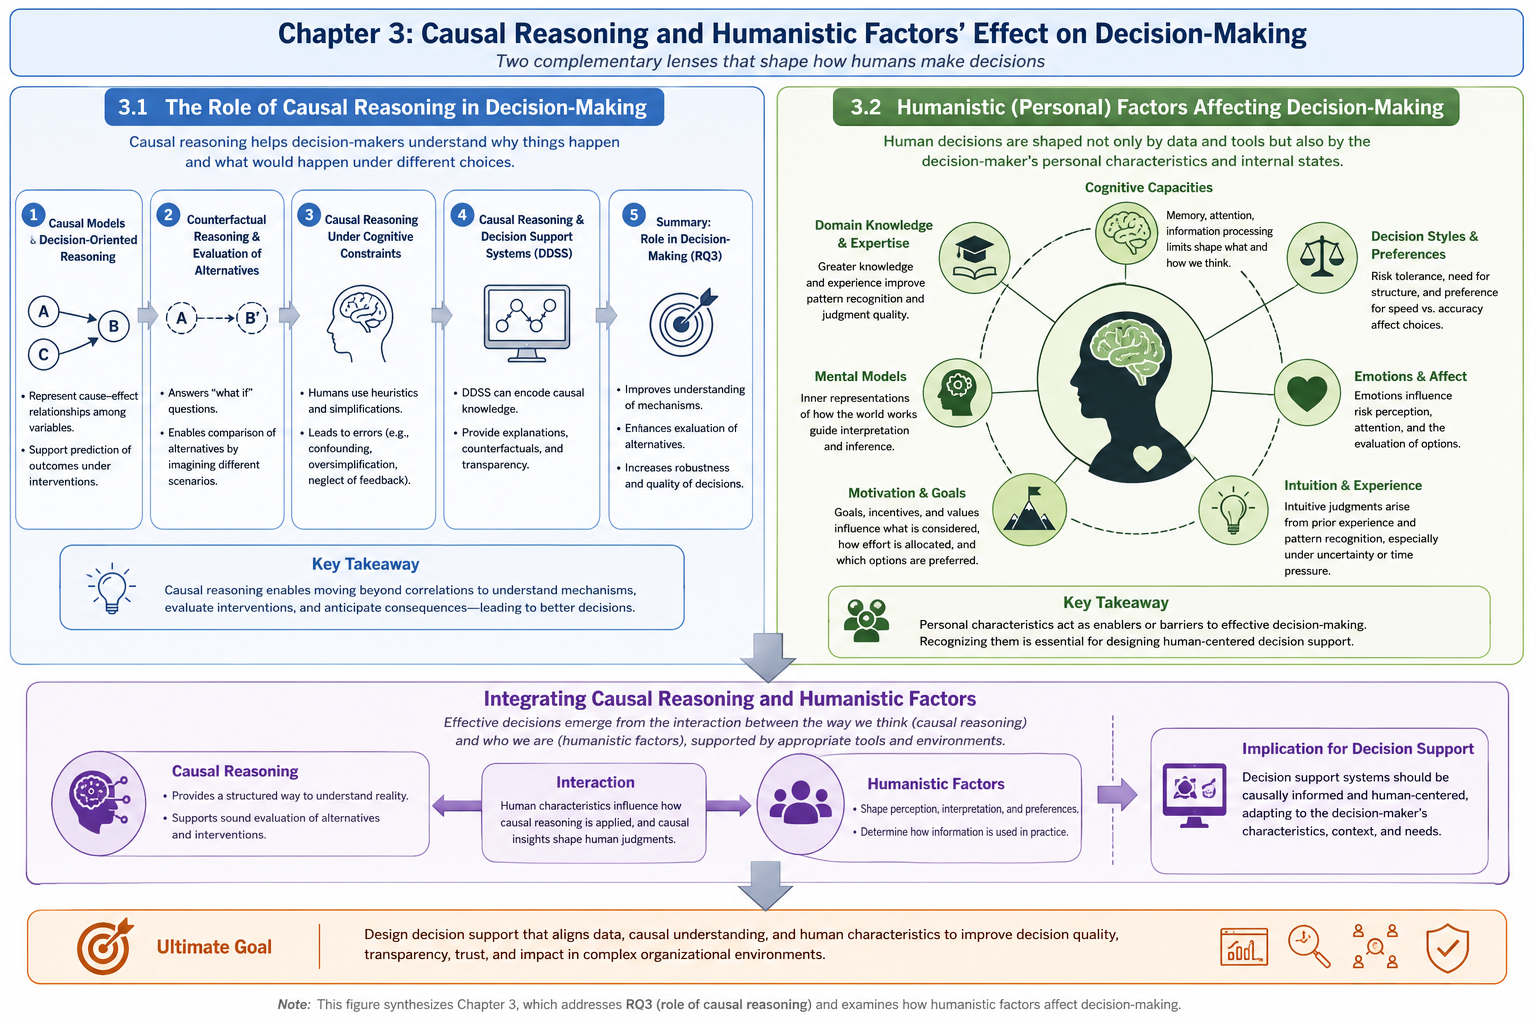
\includegraphics[width=6in]{Figures/ThirdChapterSummary.png} % ≤ 6 inches wide
    \caption[Summary of the role of causal reasoning and humanistic factors in decision-making]{Summary of the role of causal reasoning in decision-making, and how humanistic factors affect decisions. Inspired by both views, it is concluded that decision support systems (DSSs) should be causally informed and human-centered, adapting to the decision-maker's characteristics, problem's context, and task needs (generated by Gen-AI).}
    \label{HumanRoleSummary}
\end{figure}

\chapter{A Human-and-Task-Centered Framework for Integrated Application and Design of Decision Support Tools}
By reviewing the corresponding research literature on the data-driven tools and how decisions can be informed by analysis of accessible data using these tools in the two previous chapters, we learned that an effective decision-making process that solves organizational decision problems should take into account the roles of context-dependency of the data and DMs’ personal characteristics in exploiting data towards decision-making. In this chapter, we aim to synthesize this knowledge to establish a decision-making process framework that brings together the strengths of both DDTs and DMs’ prior causal knowledge of the decision domain and tailors it to the task’s nature as well as the decision-making individual’s character and cognitive capacities. What the framework actually does is to provide (i) \textbf{an overall workflow for co-application and symbiosis of DDTs throughout a generic decision-making process}, and (ii) \textbf{a process model for practical integration of DDTs within a decision support solution according to design and integration recommendations and guidelines in related bodies of research}, while these guidelines take the decision process’s end goal, the type of task at hand, and several related cognitive and personal characteristics of the decision-maker all into account. In other words, the framework tends to suggest when every DDT should be used, and how it should be used in coordination with other DDTs to support the entire organizational decision-making process. From this perspective, the framework acts similarly to \textit{Anticipatory Design (AD)} framework~\cite{cerejo2020lens, cerejo2023anticipation}, which is an effort to mollify the effect of decision fatigue through the application of machine learning and algorithmics on the decision-makers’ preference data to prioritize and filter the set of alternatives, leading to a simplified selection of the final choice.
\section{Framework's Foundation}
\subsection{Decision-Making Generic Process}
As explained in the 2\textsuperscript{nd} chapter, several models of decision-making have been introduced throughout the contemporary history of decision-making literature to shed light on both descriptive and normative accounts of decision-making through the lens of different disciplines, including mathematics, psychology, and cognitive science. As our focus in this research is to augment decision efficiency, accuracy, and confidence of organizational decision-makers, we adopt Herbert Simon’s three-stage decision-making process model ~\cite{simon1960new} as the basis for our framework because of its practical and task-oriented approach to the decision-making process.\par
\subsubsection{Decision-Making Stages and Activities}
In Simon’s model, decision-making is viewed as a process of several activities (which we may also refer to in this work as \textit{decision tasks}), accomplished across three stages that together constitute the entire decision-making process. These activities include:\par
\textbf{Stage 1. Intelligence}\par
1.1. Collect and organize data from the environment\par
1.2. Check the data for any situation requiring decision-making\par
1.3. Detect and understand the (decision) problem\par
1.4. Develop the decision problem’s statement ~\cite{phillips2013intelligent}\par
1.5. Acquire more information about the problem ~\cite{phillips2013intelligent}\par
\textbf{Stage 2. Design}\par
2.1. Develop decision criteria ~\cite{phillips2013intelligent}\par
2.2. Develop alternative courses of action ~\cite{phillips2013intelligent}\par
2.3. Identify impactful uncontrollable variables, parameters, and events ~\cite{phillips2013intelligent}\par
2.4. Specify the relationships between alternative actions, criteria, and the uncontrollable variables and events ~\cite{phillips2013intelligent}\par
2.5. Measure the relationships in a meaningful way ~\cite{phillips2013intelligent}\par
\textbf{Stage 3. Choice}\par
3.1. Evaluate each alternative’s resulting status for all criteria 
~\cite{phillips2013intelligent}\par
3.2. Analyze the sensitivity of each alternative to any extent of change in the uncontrollable variables\par
3.3. Develop/Select the final set of actions that best meet the criteria
~\cite{phillips2013intelligent}\par
In later works (e.g.,~\cite{mintzberg1977new}), a fourth stage of \textit{Implementation} was also added to Simon’s initial three-stage model to cover the activities of decision implementation, plan development, and resource allocation. We, however, consider the activities in the initial first three stages as the only points in the entire organizational decision process that are potentially subject to the application of the pre-identified DDTs. In the later sections, we will first speculate on which DDTs are most justified (based on the literature analysis in the 2\textsuperscript{nd} chapter) to assist decision stakeholders in an organization in performing different activities across all stages. We will then provide a systematic and multidimensional framework that prescribes the process of stage-level integration of the DDTs that are found relevant to a particular stage.\par
It is important to note that the sequence of the activities across the three stages is not necessarily followed in all situations; according to Simon himself, going back and forth between stages at any point might become unavoidable due to the complexity of organizational decision problems. In addition, some decision problems may arise at each stage, requiring their own cycle of Intelligence, Design, and Choice ~\cite{simon1960new}.
\subsubsection{Decision Type}
According to Simon, one of the most basic factors influencing how a decision is made concerns the notion of \textit{Type of Decision} ~\cite{simon1960new} (hereafter, we use Decision Type), that is, whether \textit{\textbf{programmed}} or \textit{\textbf{non-programmed}}. Programmed decisions are the kinds of decision problems organizations face regularly; therefore, they develop specific structures and instructions for handling and solving them when they occur ~\cite{simon1960new}. For example, Banks receive tons of applications each day for loans, mortgages, and credit, requiring the banks’ financial officers to decide whether to approve them or not. On the other hand, non-programmed decisions are ill-structured, novel problems, and often unexpected. As organizations may not have specified prior instructions to deal with such kind of decisions accordingly, they need to use general problem-solving skills and bring their extra knowledge into play to solve the problem ~\cite{simon1960new}. Policy decisions—those that require DMs to analyze the possible impacts and consequences of taking a set of actions as a response to a unique or unusual problem—are the best identifier of this decision type. Looking back at the three-stage decision process model, if the type of the decision on hand is programmed, we can anticipate in general that the activities inside the Intelligence stage are skipped (as the decision problem is fully known), and those inside the Design stage are only executed ad hoc. However, if the decision is non-programmed, the execution of the Design stage’s activities is essential for accomplishing the entire decision-making process.

\subsection{Mapping Data-Driven Tools to Decision Stages}
To produce a unified process framework aiming to guide the integrative application and design of tools from a diverse set of tool families (i.e., DDTs) to support the decision-making process, we first need to specify the stages or activities in the generic decision-making process at which these tools are commonly applied. Therefore, we map DDTs to the three stages according to the conceptual relevance of the DDTs' common decision use-cases (derived in the 2\textsuperscript{nd} chapter as a result of the DDDM literature review) to the decision stages' activities and end goals described above. Figure ~\ref{DDTAssignment} illustrates the map of conceptual relationships between DDTs and the decision stages.\par
\begin{figure}
    \centering
    % Ensure figure width fits within SFU margins
    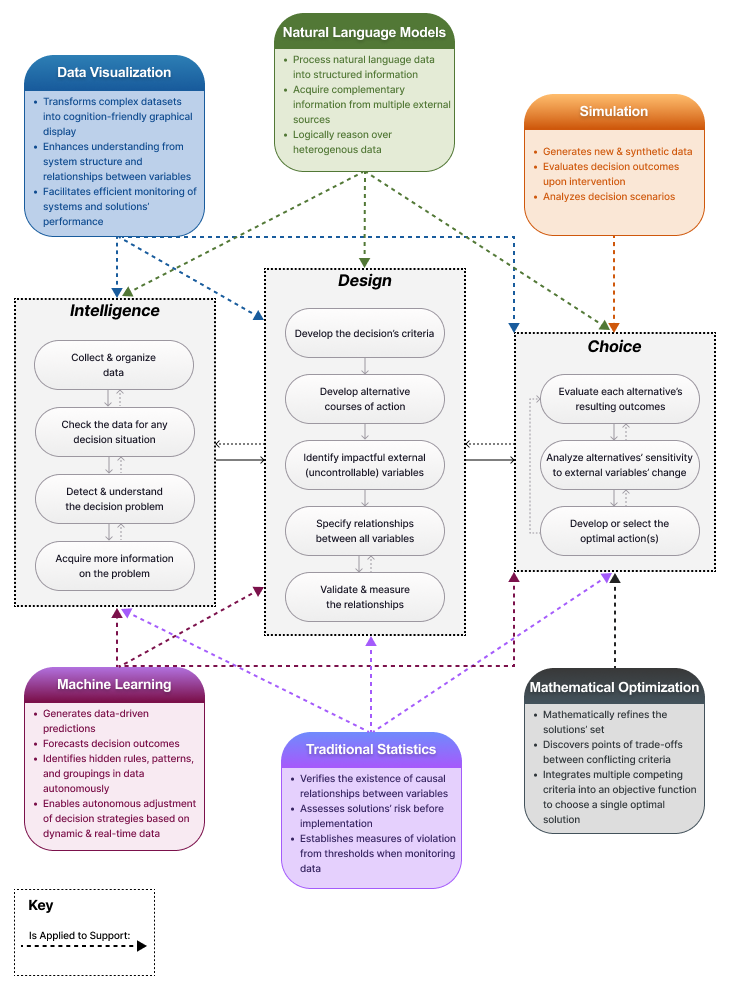
\includegraphics[width=6in]{Figures/DDTAssignment.png} % ≤ 6 inches wide
    \caption[Mapping DDTs to decision stages]{The map of conceptual relationships between the decision use-cases of identified data-driven tools (DDTs) and the decision stages in Simon's decision-making process model}
    \label{DDTAssignment}
\end{figure}
In the visual map of Figure ~\ref{DDTAssignment}, we did not include \textit{problem statement development} as it is more of a manual task concerned with the documentation of decision problem discovery that is realized through the Intelligence stage.\par
As the derived use-cases of data visualization for decision-making suggest, it can aid decision-makers in accessing a large chunk of data at once, enabling them to recognize patterns and more abstract information more efficiently. This then justifies the application of data visualization in the Intelligence stage to \textit{check the data for the decision problem}, as well as to \textit{detect and understand the decision problem}. Data visualization also facilitates understanding the system and data structure, making it a suitable tool to \textit{specify relationships} that might become increasingly complex between \textit{decision alternatives, outcomes,} and \textit{other uncontrollable and external factors} throughout the Design stage. The same communicative aspects of data visualization can also play a role in aiding decision-makers to better understand and imagine the possible outcomes of each decision alternative during the Choice stage, as well as the solutions’ sensitivity and tolerance to external occurrences.\par
Unsupervised machine learning techniques are essentially engaged in detection and clustering of natural groupings, similar themes, and anomalies within unlabeled data, seemingly in accordance with the task of \textit{detection and understanding the decision problem} in the Intelligence stage. Supervised machine learning techniques are also useful when it comes to forecasting trends inside the labeled data, making them a good match for the task of \textit{detection and understanding the decision problem} in the Intelligence stage. We also saw that supervised ML techniques are used to autonomously extract and verify mathematical associations and/or causal relationships between data variables. Therefore, the \textit{relationship measurement} task inside the Design stage is a potential context in which supervised ML techniques can assist decision-makers. The prediction power of supervised ML techniques makes them capable of generating numerical outcomes for possible interventions; hence, we also map them to \textit{evaluating each alternative’s outcomes} task in the Choice stage.\par 
Natural language models are capable of transforming natural language data into a structured, actionable format, assisting in the Intelligence stage’s activities when the data is in the form of human natural language. Modern LLMs provide complementary information about any problem from external sources like the web in the form of human natural language. This is particularly useful at the end of the Intelligence stage when \textit{more information on the decision problem} is needed for the later tasks of decision criteria and alternatives development. LLMs can also aid decision-making teams in generative tasks inside the Design stage that require brainstorming, such as \textit{decision alternatives and criteria development} and \textit{identification of uncontrollable events and variables}. In addition, LLMs’ reasoning capability makes them a useful tool to evaluate the possible outcomes. Since LLMs can provide an explainable rationale behind selecting a choice, decision-makers might be willing to use them in \textit{the selection of the final set of actions} at the end of the Choice stage.\par
All the different methods of simulation have the goal of mathematically generating synthetic data from some input data in common. This makes them a key tool for \textit{prediction and evaluation of decision alternatives’ resulting outcomes} in the Choice stage. \textit{Analyzing the sensitivity of the solutions} to any change in external variables can also be aided by simulating the effect of these changes on the outcomes of each decision alternative/solution.\par 
Mathematical optimization frameworks formalize any decision problem as a mathematical optimization process through which a single solution or a set of non-dominant solutions among all collected solutions are autonomously selected with minimum human intervention. Multi-criteria decision-making (MCDM) methods, either from the MADM (multi-attribute decision-making) category or from MODM (multi-objective decision-making), seek to find the optimal choice as an alternative/solution for the decision problem. Therefore, they are particularly useful for automating the task of \textit{selection/development of the final set of actions} at the end of the Choice stage.

\subsection{Existing Researches on the Application of Data-Driven Tools for Intelligence} \label{ExistingResearchIntelligence}
As described earlier, decision stakeholders seek to capture and frame a decision problem by consistently monitoring collected and organized data. We also observed that this process is primarily aided by data visualization, ML, statistical models, and natural language models from the set of our labeled DDTs. In fact, the majority of the studies’ focus has been on the application of these tools (particularly data visualization) for facilitating the intelligence stage of Simon’s decision-making model ~\cite{dimara_critical_2022}. Therefore, human-centric and integrative approaches are already present that can lay the foundation for a more holistic decision support framework. The \textbf{visual analytics} body of research is dedicated to integrating interactive visualization and data analytics tools to help humans make sense of data, making it fully compatible with our goal of proposing a cross-tool synthetic workflow to augment the Intelligence stage’s activities.

\subsubsection{Visual Analytics for Sense-making}
Visual Analytics (VA) is the science of analytical reasoning facilitated by interactive visual interfaces ~\cite{thomas2005illuminating}. VA combines automated analysis techniques with interactive visualizations for an effective understanding, reasoning, and decision-making on the basis of very large and complex data sets ~\cite{keim2008visual}. It fundamentally supports the intelligence stage through structured sense-making processes, where users iteratively move between data exploration and hypothesis refinement. The recent \textit{Iceberg} sense-making model from Berret and Munzner~\cite{berret2024iceberg} conceptualizes this as a progression from surface-level observations to deeper latent structures, emphasizing iterative abstraction and validation. Similarly, sense-making is characterized as a knowledge-generation process, where insights emerge through continuous interaction between user cognition and external visual representations ~\cite{vuckovic2022sense}. This process has been illustrated in Figure ~\ref{VAProcessModel} from Ltifi et al.~\cite{ltifi2020adapted}, in which an initial analysis, depending on the nature of the dataset, is performed and generates a visual display that can aid the user’s perception in deriving new insights from the data. The user builds hypotheses about the data based on the gained knowledge, making him/her to re-explore the data to confirm them via new specifications provided to the visualization system. This specified visualization again causes new insights to be derived and merged into the user’s knowledge. In the context of VA’s knowledge-generation process, the application of the DDTs that we found to have a conceptual relationship with the Intelligence stage activities can be further studied in an integrated approach, as we will be doing in the following sections.
\begin{figure}
    \centering
    % Ensure figure width fits within SFU margins
    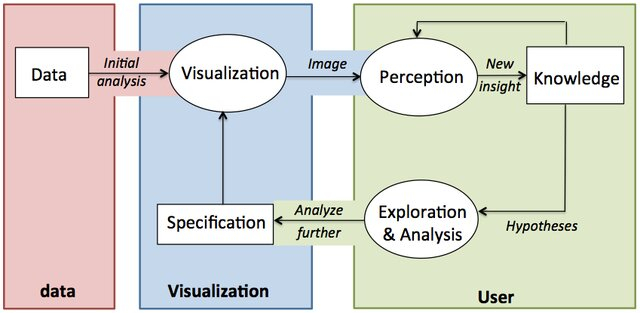
\includegraphics[width=6in]{Figures/GenericVisualAnalyticsProcess.jpg} % ≤ 6 inches wide
    \caption[Visual analytics' generic pipeline]{Generic pipeline of visual analytics (VA), as initially introduced by Van Wijk ~\cite{van2005value} (adopted directly from Ltifi et al.~\cite{ltifi2020adapted}).}
    \label{VAProcessModel}
\end{figure}
\subsubsection{The Role of Interactive Visualization in Intelligence}
From the VA point of view, visualizations act as external cognitive artifacts, enabling users to offload memory, compare alternatives, and detect anomalies that would otherwise remain hidden ~\cite{sedig_supporting_2016}. This aligns directly with the intelligence stage’s need for signal detection and problem framing. Results of the literature review in the 2\textsuperscript{nd} chapter showed that visualization dashboards involving multiple juxtaposed or coordinated views are frequently employed to enable users to interactively switch between different visualization structures for maximum exposure to different aspects of a dataset. \textbf{Interactive dashboards} serve as the primary interface through which stakeholders \textbf{engage with data, aiming to gain new insights} or \textbf{validate previous hypotheses}. In Figure ~\ref{VADashboard}, an interactive dashboard from a VA system developed and presented by Al-Hajj et al.~\cite{al2013visual}, to aid in a healthcare decision-making process based on injury data in British Columbia (BC). Multiple views, such as geospatial maps, line graphs, and stacked bar graphs, have been juxtaposed all in one interface (shown in Figure ~\ref{VADashboard}), enabling healthcare planners to explore different aspects of the dataset simultaneously for a more accurate judgment and a quality decision to be made.\par
\begin{figure}
    \centering
    % Ensure figure width fits within SFU margins
    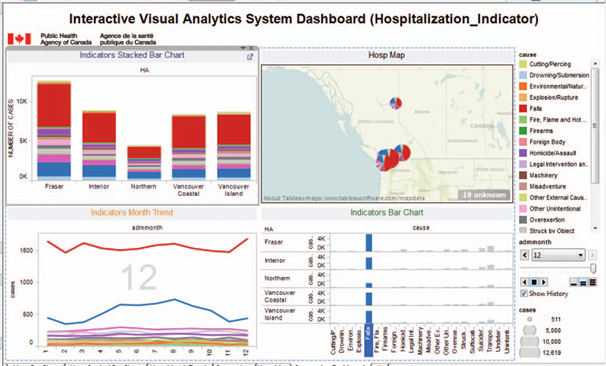
\includegraphics[width=6in]{Figures/VADashboardPublicHealth.png} % ≤ 6 inches wide
    \caption[An interactive VA dashboard example]{An example of an interactive dashboard in a visual analytics (VA) system for public health decision-making (adopted directly from Al-Hajj et al.~\cite{al2013visual}).}
    \label{VADashboard}
\end{figure}
The dataset may exhibit heterogeneous structures and contain attributes with varying data types, necessitating the implementation of diverse dashboard views that are compatible with the underlying data characteristics while ensuring flexibility and comprehensiveness. In the VA system’s dashboard presented in Figure ~\ref{VADashboard} as an example, a 2D map has been employed to visualize the location of different BC hospitals as geospatial data (top-right view), whereas a multi-line graph has been embedded as well to visualize the temporal patterns and trends in values of health indicators over time, which is time-series data (bottom-left view).\par
Moreover, some interactive VA dashboards, such as \textit{Cosmos}, introduced by Dowling et al.~\cite{dowling_interactive_2019}, allow users to explore large corpora, extract themes, and detect emerging narratives from plain-text documents as an unstructured dataset.\par
The combination of the above two cases has also been realized in the \textit{TimeSets} VA system (from Xu et al.~\cite{xu_timesets_2020}), enabling analysts to identify temporal patterns and evolving events in social media text messages as unstructured data, which are critical for intelligence analysis tasks.\par
In general, VA systems are expected to aid users in \textbf{exploratory data analysis (EDA)}, temporal and multivariate pattern detection ~\cite{soriano2020tv}, and cross-filtering and brushing interactions ~\cite{roberts2007state}, by means of linked visual representations.\par
As new insights from visualization are derived by performing finer-level data tasks such as \textit{correlation} and \textit{anomaly detection}, \textit{distribution characterization}, \textit{value comparison}, etc., a key design principle is the visibility and complementarity of interactions, where multiple coordinated views (e.g., scatterplots, networks, timelines) provide complementary perspectives on the same dataset, enhancing cognitive integration ~\cite{sedig_supporting_2016}.
\subsubsection{The Integration of Data Analytics Methods and Visual Analytics Systems}
In the VA-aided sense-making process model, data analytics methods, either from the traditional statistical (TS) analysis class of techniques or from modern ML methods, have been largely applied to \textbf{perform initial analysis over the raw dataset, in-depth analysis over the visualized data,} and \textbf{hypothesis generation and validation based on the user’s knowledge and assumptions}. Therefore, we hereby investigate the practical implications of how TS and ML classes of tools are, or can be, generally integrated with interactive visualization systems to exploit the capacities of all three DDTs (VIZ + TS/ML) in augmenting the process of transformation from raw data to knowledge, leading to discovery and understanding of a plausible decision problem.\par
\noindent\textbf{\textit{Traditional Statistics (TS) Methods and Visual Analytics Systems}}\par
Several studies have incorporated different types of statistics in their proposed VA systems, aiming to facilitate EDA, hypothesis generation and validation, correlation and regression analysis, and uncertainty quantification.\par
Kale et al.~\cite{kale2023evm} have developed a VA system to help users visually assess the similarity of the distribution of the observational data on hand with the distribution of a set of randomly generated data points based on the users’ choice of model (e.g., \textit{normal} or \textit{logistic}), leading to the formation of hypotheses about the dataset’s nature and characteristics. As shown in Figure ~\ref{DataDistributionHypothesis}, their system interface consists of four panels including (A) \textit{shelf construction }panel for selection of data features to be visualized, (B) \textit{filters and transformation} panel to restrict or alter the visualized data, (C) \textit{chart} panel for visualizing pre-specified data in the form of hardcoded chart types, and (D) \textit{model bar} panel that allows user to specify the distribution type of the random data to be generated as baseline for distribution comparison. The system also allows the user to visually explore the hypotheses about the association between variables by juxtaposing multiple views of the filtered dataset (see Figure 1.B in Kale et al.~\cite{kale2023evm}).\par
\begin{figure}
    \centering
    % Ensure figure width fits within SFU margins
    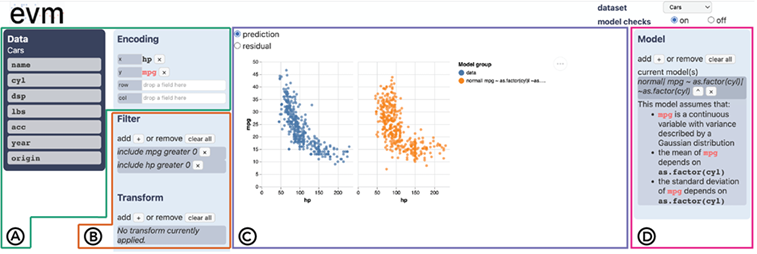
\includegraphics[width=6in]{Figures/DistributionHypothesis.png} % ≤ 6 inches wide
    \caption[An interactive VA system for exploratory visual modeling of data]{Exploratory Visual Modeling (EVM): An interactive visual analytics (VA) system that facilitates the generation of hypotheses about the data distribution (adopted directly fromKale et al.~\cite{kale2023evm}).}
    \label{DataDistributionHypothesis}
\end{figure}
Another prominent integration of traditional statistics with interactive visualization for EDA and hypothesis testing has been introduced by Majumder et al.~\cite{majumder2013validation}, wherein users are able to visually test the veracity of their hypotheses with the aid of inferential statistics and data simulation. In Figure ~\ref{LineupProtocol}, the overall process of their visual inference method (i.e., \textit{Lineup protocol}) has been shown against the process of conventional statistical inference. Given the user wants to test whether the difference between mean values of a numerical variable for two separate values of a categorical variable (e.g., the difference between the mean height of men and women) is statistically significant, the system generates several lined-up side-by-side box plots, each representing a hypothetical scenario of a data distribution affirming the initial null hypothesis (H\textsubscript{0}), and randomly embeds the box plot of the actual data distribution among them. If the user successfully identifies and selects the box plot of the actual distribution, H\textsubscript{0} is rejected. Majumder et al.~\cite{majumder2013validation} showed that users’ accuracy in this method of visual inference is comparable to the test results of conventional inference, making it a reliable choice for circumstances in which conventional inferential statistics methods are not applicable.\par
\begin{figure}
    \centering
    % Ensure figure width fits within SFU margins
    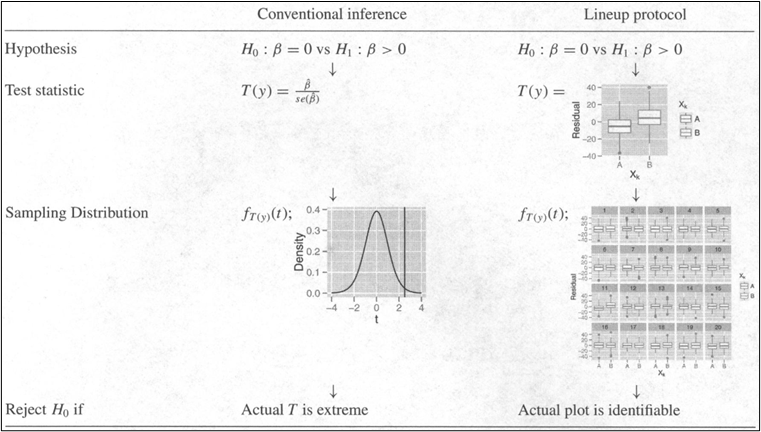
\includegraphics[width=6in]{Figures/LineupProtocol.png} % ≤ 6 inches wide
    \caption[Lineup protocol: An example of VA-aided hypothesis validation]{Comparing the interactive-visualization-aided Lineup protocol's process with the conventional inference for hypothesis validation (adopted directly from Majumder et al.~\cite{majumder2013validation}).}
    \label{LineupProtocol}
\end{figure}
Despite being studied only for a specific case of the two-sample t-test while having one categorical variable and one numerical variable, the idea behind the visual inference process designed by Majumder et al.~\cite{majumder2013validation} can be further explored for possible extensions and integration within the entire VA-aided sense-making process as one of the mechanisms for hypothesis validation and insight generation.\par
The integration of exploratory and descriptive statistical techniques within a VA system was demonstrated by \textit{Multidimensional Data eXplorer (MDX)}, introduced by Steed et al.~\cite{steed2014visual} to support visual data mining through coordinated analytical and visualization capabilities. As the MDX system has been primarily developed to facilitate the comparison between multiple items (e.g., cars) in several dimensions (e.g., MPG, acceleration, etc.), it incorporates parallel coordinated plots (PCPs) as the base visualization structure and embeds additional visual encodings, in terms of both coordinated graphs and text, on the screen to indicate various statistical measures. The visual marks and channels of the PCP (e.g., parallel coordinate axes) themselves are also customizable, and the user can switch between multiple representations to explore different aspects of the data. Figure ~\ref{MDX} illustrates a PCP view of MDX, summarizing the variability and central tendency of all data attributes.\par
\begin{figure}
    \centering
    % Ensure figure width fits within SFU margins
    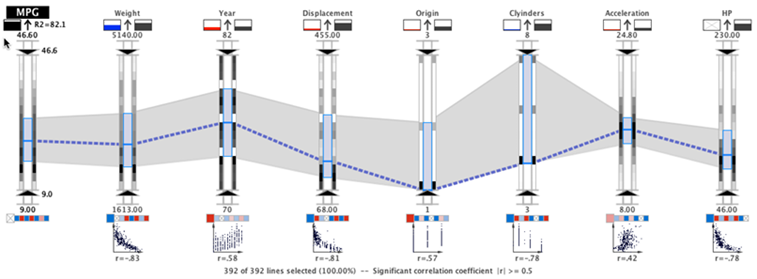
\includegraphics[width=6in]{Figures/MDX.png} % ≤ 6 inches wide
    \caption[A statistics-powered example of an interactive VA system]{Multidimensional Data eXplorer (MDX): An interactive visual analytics (VA) system that utilizes exploratory and descriptive statistics for facilitating insight generation from data (adopted directly from Steed et al.~\cite{steed2014visual})}
    \label{MDX}
\end{figure}
In Figure ~\ref{MDX}, every vertical coordinate axis is a channel that encodes the range and distribution of values for a particular dimension of the cars’ dataset (e.g., MPG), using light-blue box plots. These box plots encode the median and interquartile values of every dimension, facilitating the exploration of every data attribute’s distribution. The user, however, can set these box plots to represent the mean (instead of the median) and standard deviation (instead of the quartiles) of the values of every dimension. This particular PCP view shows the overall central tendency and variability measures with a gray polygon connected between the axes and a blue-gray dashed line. Minimum and maximum values of every dimension have also been shown above and below the vertical axis associated with the dimension (e.g., the maximum value of MPG between all the cars is 46.60, while the minimum is 9.00).\par
Not only the data variability and distribution but also the exploration of the variables’ correlation is supported by the MDX system on the same PCP view. The user can assess how associated a variable, such as MPG, is with another variable like Acceleration using the correlation indicator blocks below the variable’s axis. The selection of every colored square-shaped block results in rendering a 2D scatterplot, of which the horizontal axis encodes the values of the attribute above the block, and the vertical axis encodes the values of the attribute that has been placed in the PCP in the same order as the block. Correlation coefficients between the two variables have also been calculated using Pearson’s r and are represented below the rendered scatterplot.\par
Despite being solely placed on the basis of one chart type (PCP), the MDX system is a decent example of how a VA system can incorporate statistical techniques for enhancing sense-making through interactive data exploration. Several low-level data tasks, such as finding correlation and regression, characterizing data distribution, detecting anomalies, and identifying clusters/classes in data, can all be supported within a single statistics-aided VA system.\par
Lastly, certain statistical techniques can be integrated within VA systems for quantification of the uncertainty in the insights derived from the EDA process to control users’ false discovery rate ~\cite{sarma2024odds}. Sarma et al.~\cite{sarma2024odds} have shown that the application of statistical correction procedures (e.g., Benjamini-Hochberg) in a VA context can effectively control the ratio of false positive errors to the total number of null hypothesis rejections when multiple hypotheses are tested by the user.\par
\noindent\textbf{\textit{Machine Learning (ML) Models and Visual Analytics Systems}}\par
ML models and algorithms are mainly applied in the Intelligence stage for \textbf{preprocessing both structured and unstructured data}, as well as assisting the user with analytical exploration of visualized data. ML methods, however, support preprocessing differently for structured and unstructured data (text, image, audio, etc.) because the nature of the data, the preprocessing objectives, and the analytical challenges are fundamentally different. Therefore, we hereby investigate the role of ML algorithms in preprocessing each of these types of data structures separately.\par

\noindent\textit{ML-aided Visual Analytics for Preprocessing of Structured Data}\par
Research publications indicate that ML models support structured data preprocessing in VA systems by \textbf{automating data transformation, reducing dimensionality, detecting anomalies, clustering, selecting features, imputing missing values}, and assisting analysts in preparing datasets for subsequent exploration and modeling.\par 
One of the most common ML-supported preprocessing operations in VA systems is \textbf{dimensionality reduction (DR)}. DR algorithms such as PCA, t-SNE, UMAP, and self-organizing maps transform high-dimensional structured datasets into lower-dimensional representations suitable for interactive visualization.\par
ML models are also employed for \textbf{automated feature selection} during the preprocessing of structured data. In many VA systems, statistical learning methods rank variables according to predictive relevance, correlation structure, or redundancy. The resulting feature subsets are then visualized through heatmaps, scatterplots, parallel coordinates, or correlation matrices to support analyst interpretation.\par
Another important role of ML in structured-data preprocessing is \textbf{anomaly and outlier detection} within the raw dataset. Clustering algorithms, density estimation models, and isolation-based methods are frequently employed before VA interfaces to identify and substitute or remove suspicious records, noisy data, or rare events. Visualization components subsequently allow analysts to inspect detected anomalies and determine whether they represent meaningful signals or preprocessing artifacts. This combination improves data quality while preserving analyst oversight ~\cite{endert_state_2017}.\par
Research publications further show that ML-assisted preprocessing supports \textbf{data transformation and representation learning}. Kasik et al.~\cite{kasik_data_2009} explain that VA systems rely on computational transformations that convert raw structured data into concise and visually interpretable representations. These transformations may involve scaling, aggregation, encoding, projection, or learned representations generated through ML techniques. The transformed representations then become suitable for interactive visual exploration.\par
The literature also highlights that \textbf{ML-supported preprocessing enhances scalability} when VA systems handle large structured datasets. Endert et al.~\cite{endert_state_2017} describe how ML methods help reduce analytical complexity by filtering, summarizing, and organizing high-dimensional data before visualization. These preprocessing steps reduce visual clutter and improve cognitive interpretability for analysts working with complex datasets ~\cite{endert_state_2017}.\par

\noindent\textit{ML-aided Visual Analytics for Preprocessing of Unstructured Data}\par
Research publications indicate that ML models play a central role in preprocessing unstructured data within VA systems by transforming raw text, images, audio, video, and graph-based content into structured or semi-structured representations suitable for computational analysis and interactive visualization. In contrast to structured datasets, unstructured data lacks predefined schemas and therefore requires extensive \textbf{semantic extraction, representation learning}, and \textbf{dimensional transformation} before visualization can occur. Preprocessing of unstructured data can be viewed as a multi-stage pipeline involving \textbf{feature extraction, semantic modeling, representation learning, filtering}, and \textbf{summarization}. ML techniques—particularly deep learning, clustering, and topic modeling—are widely used as the core of NLP engines to accomplish these transformations.\par
A foundational role of ML in unstructured-data preprocessing is \textbf{feature extraction} and \textbf{representation learning}. Raw unstructured data cannot usually be visualized directly because it lacks explicit attributes or dimensions. ML models, therefore, convert the data into machine-readable feature spaces. For textual data, preprocessing commonly includes tokenization, stemming, named entity recognition, document embeddings, semantic similarity computation, and topic extraction. For image and video data, \textit{convolutional neural networks (CNNs)} extract latent visual features, object categories, and semantic descriptors. These extracted representations subsequently become suitable for interactive visualization and analysis. Research surveys on visual analytics and ML integration emphasize that representation learning is one of the primary enabling mechanisms allowing unstructured content to enter VA pipelines ~\cite{yuan2021survey}.\par
\textbf{Topic modeling} constitutes one of the most widely discussed ML-supported preprocessing approaches for textual VA systems. Probabilistic topic models such as latent Dirichlet allocation (LDA) transform large document corpora into structured topic distributions that can be visually explored through temporal views, topic maps, cluster graphs, and document-topic relationships. For example, the well-known VA system \textit{ThemeRiver}—introduced for the first time by Havre et al.~\cite{havre2002themeriver}—preprocesses textual streams into thematic representations that allow users to visually analyze topic evolution over time.\par
\begin{figure}
    \centering
    % Ensure figure width fits within SFU margins
    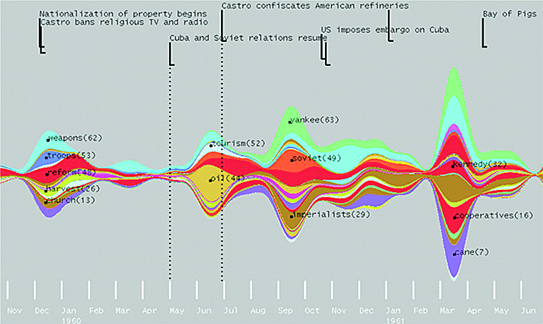
\includegraphics[width=6in]{Figures/ThemeRiver.png} % ≤ 6 inches wide
    \caption[A ML-aided VA system example for topic extraction and modeling]{\textit{ThemeRiver}'s interface: The strength (frequency) of the topics in Fidel Castro's speeches, interviews, and articles over two years has been extracted and modeled with the aid of ML algorithms (adopted directly from Havre et al.~\cite{havre2002themeriver}).}
    \label{Themeriver}
\end{figure}
In Figure ~\ref{Themeriver}, a screenshot from one of \textit{ThemeRiver}'s views has been illustrated in which the fluctuations in strength of every individual topic theme in Fidel Castro’s collection of speeches, interviews, and articles have been visualized over a year-and-a-half period of time in the early 1960s. The different extracted topics from Castro’s collection in Figure ~\ref{Themeriver} have been differentiated by their background color, while the vertical width of every colored region at any point in time represents the frequency of the corresponding topic’s instances at that given time.\par
Research publications also show that \textbf{clustering algorithms} are frequently used to preprocess unstructured datasets into visually interpretable groups. Text documents, images, or social media posts are embedded into vector spaces using ML methods and subsequently grouped according to semantic similarity. The resulting clusters form the basis for interactive visualizations such as scatterplots, force-directed graphs, hierarchical trees, and heatmaps. An example of a VA system that leverages ML clustering techniques for semantic grouping of text data is \textit{TimeSets}, which was proposed by Xu et al.~\cite{xu_timesets_2020}. In Figure ~\ref{TimeSets}, we have shown a view of \textit{TimeSets} that visualizes different clusters of topics in a file by different background colors.\par
\begin{figure}
    \centering
    % Ensure figure width fits within SFU margins
    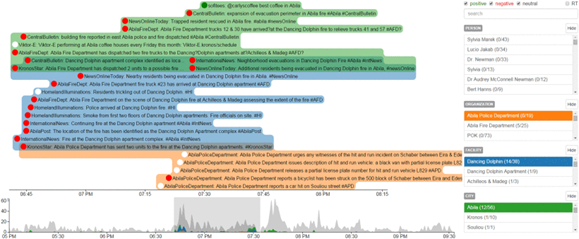
\includegraphics[width=6in]{Figures/TimeSets.png} % ≤ 6 inches wide
    \caption[A ML-aided VA system example for topic clustering]{\textit{TimeSets}' interface: The different topics inside a text file have been extracted and visually classified with distinct background colors with the aid of ML clustering algorithms (adopted directly from Xu et al.~\cite{xu_timesets_2020})}
    \label{TimeSets}
\end{figure}
Same as for structured data, \textbf{dimensionality reduction (DR)} is another major preprocessing mechanism for unstructured data in VA systems. Since textual embeddings, image descriptors, and learned latent representations are often high-dimensional, DR algorithms such as PCA, t-SNE, and UMAP are used to project the data into two- or three-dimensional visual spaces. This preprocessing enables analysts to visually inspect semantic similarity, clusters, anomalies, and conceptual neighborhoods within unstructured datasets.\par
Deep learning models have increasingly been adopted for preprocessing multimodal unstructured data. Autoencoders, transformers, \textit{recurrent neural networks (RNNs)}, and \textit{CNNs} generate latent embeddings that \textbf{summarize the semantic characteristics} of text, audio, and images. These learned embeddings are subsequently visualized to support exploratory analysis and sense-making. Research on visual analytics for deep learning notes that latent-space representations significantly improve analysts’ ability to explore complex semantic relationships in unstructured datasets.\par
Another important preprocessing function supported by ML is \textbf{semantic filtering} and \textbf{relevance detection}. VA systems that process social media streams, intelligence reports, biomedical literature, or news corpora frequently use supervised or semi-supervised ML classifiers to identify relevant documents, remove noise, and prioritize meaningful content before visualization. This reduces cognitive overload and allows analysts to focus on semantically important information. Endert et al.~\cite{endert_state_2017} argue that ML-driven filtering mechanisms are essential for scaling VA systems to large unstructured datasets.\par
Finally, \textbf{named entity recognition (NER)} and relation extraction models are also heavily utilized during the preprocessing of textual data. These NLP methods identify entities such as people, organizations, locations, and events from raw text and transform them into structured relational networks suitable for node-link diagrams and graph visualizations. Numerous intelligence-analysis and investigative VA systems rely on ML-based entity extraction pipelines to convert narrative documents into analyzable graph structures.\par
\noindent\textit{ML-aided Exploratory Visual Data Analysis}\par
Beyond preprocessing, research publications also indicate that ML models support the EDA process in VA systems by \textbf{suggesting exploration pathways, recommending next analytical steps, assisting verification processes}, and \textbf{mitigating cognitive biases} ~\cite{endert_state_2017}. In this category, Multu et al.~\cite{mutlu2021towards} have proposed a task-based VA tool that employs a rule-based ML model to recommend appropriate visualizations for a tuple of user-selected attributes, as well as a sequence of interactions (paths) for the user’s current task. Figure ~\ref{taskRecommend} shows the interface of their system in which AI-driven recommendations are generated in multiple stages. Stage A shows how to choose the attributes to be visualized. Stage B lists the appropriate visualizations that are automatically recommended by the rule-based system for the selected attributes. Stage C lists the recommended sequence of interactions (paths) for the user’s current task. Stage D provides a preview of a visualization that shows the outcome of the selected path. Once the user accepts the recommendation, the final visualization is shown in stage E.\par
\begin{figure}
    \centering
    % Ensure figure width fits within SFU margins
    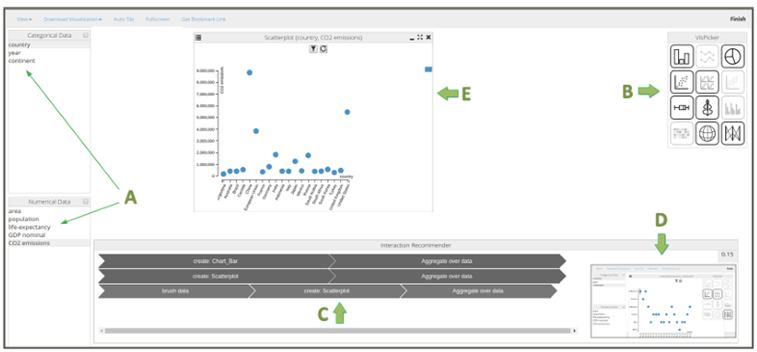
\includegraphics[width=6in]{Figures/TaskRecommMLVA.png} % ≤ 6 inches wide
    \caption[A VA system example for ML-aided view selection and task recommendation]{Task-based visual analytics tool: Panel A shows how to choose the attributes to be visualized. Panel B lists the appropriate visualizations that are automatically recommended by our rule-based system for the selected attributes. Panel C lists the recommended sequence of interactions (paths) for user’s current task. Panel D provides a preview of a visualization that shows the final outcome of the selected path. Once the user accepts the recommendation, the final visualization is shown in panel E (adopted directly from Multu et al.~\cite{mutlu2021towards}).}
    \label{taskRecommend}
\end{figure}
Generally speaking, after preprocessing has transformed the data into analyzable forms, ML models become tightly integrated with interactive visualization components to support iterative sense-making and analytical reasoning. However, when it comes to the application of analytical tools to support the user’s sense-making based on visualization, the line between modern ML models and traditional statistical techniques is blurred. This ambiguity arises because many analytical techniques commonly associated with ML originated in statistics and continue to serve both predictive and explanatory purposes. For example, regression models, clustering algorithms, dimensionality reduction (DR) methods, and Bayesian approaches are frequently categorized as ML techniques, yet they are also well-established statistical methods. In practice, the distinction often depends less on the underlying algorithm than on its intended purpose. As described earlier, statistical approaches are generally employed to explain relationships, estimate parameters, quantify uncertainty, and test hypotheses, whereas ML approaches primarily emphasize prediction, pattern discovery, and generalization to unseen data. Consequently, VA systems can incorporate analytical models that simultaneously support statistical inference and machine learning-driven exploration.\par
\noindent\textit{VIZ4ML: User-steered ML through Interactive Visualization}\par
The above-explained ML-aided preprocessing operations on both structured and unstructured data are increasingly treated as interactive and iterative tasks where \textbf{ML techniques and visualization mutually reinforce one another} to make the process for the analysts more interpretable. For example, Sacha et al.~\cite{sacha_visual_2016} have identified several scenarios wherein the DR algorithms are interactively adjusted, refined, or manipulated by the user through interactive visualization interfaces. These interaction scenarios include, but are not limited to, the selection of a proper DR algorithm, specification of algorithmic constraints and parameters, and selection of the most relevant features. These functionalities are achieved by different interaction idioms (e.g., \textit{annotations, sliders, toggle switches}, etc.) that are typically present on VA systems’ interfaces ~\cite{sacha_visual_2016}.\par
\noindent\textit{VIZ4ML: Interpretable ML through Visualization}\par
Visualization plays a critical role in making ML outputs interpretable. Visualization tools such as \textit{feature importance plots, saliency maps}, and \textit{partial dependence plots} allow users to understand model behavior and validate findings ~\cite{chatzimparmpas2020survey}. Spinner et al.~\cite{spinner2019explainer} have proposed \textit{explAIner}, a VA system that enables users to understand ML models and their limitations using different explainable AI techniques, such as \textit{local interpretable model-agnostic explanations (LIME)} and \textit{saliency maps}. Figure ~\ref{explAIner} demonstrates a screenshot of the results of a couple of explainer components used in the \textit{expAIner} system (figures on the top of every card), followed by the explainer’s verbal description (paragraphs beneath the figures).\par
\begin{figure}
    \centering
    % Ensure figure width fits within SFU margins
    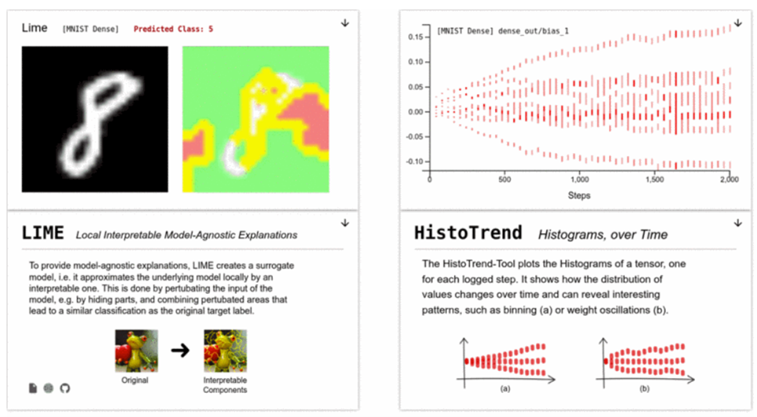
\includegraphics[width=6in]{Figures/explAIner.png} % ≤ 6 inches wide
    \caption[The application of XAI techniques for enhanced interpretability of ML algorithms]{\textit{ExplAIner}'s interface: The application of two visualization-based explainable artificial intelligence (XAI) techniques (\textit{LIME}, and \textit{HistoTrend}) for enhanced interpretability of ML pipelines (adopted directly from Spinner et al.~\cite{spinner2019explainer}).}
    \label{explAIner}
\end{figure}
Interpretability of machine learning outputs is important in visual analytics systems because analysts must be able to understand, assess, and trust the insights generated by computational models before incorporating them into their decision-making process. Visual analytics is founded on a synergistic partnership between human reasoning and automated analysis; therefore, opaque model outputs can hinder effective sense-making, reduce user trust, and make it difficult to identify model errors or biases. As noted by Endert et al.~\cite{endert_state_2017}, successful human–AI collaboration requires transparency in how analytical results are produced, so that users can validate findings, refine hypotheses, and steer the analytical process interactively.\par
\noindent\textit{ML4VIZ: Enhancing Visualization Itself with ML}\par
Recent advances in ML4VIS demonstrate how ML can optimize visualization design, recommend views, and automate insight generation, thereby accelerating intelligence activities ~\cite{wang2020applying}. In this line of research, Qian et al.~\cite{qian2022personalized} have developed a framework architecture that leverages \textit{deep neural networks (DNNs)} for learning patterns of users and their visualization preferences. Their introduced network learns such patterns based on the dataset type, visualizations previously viewed by the user, clicked visualizations, manually created visualizations, and interaction histories from many users. The system then recommends visualizations personalized to the user's preferences and analytical interests.
\subsubsection{The Integration of Language Models and Visual Analytics Systems}
The NLM DDT encompasses a broad set of ad hoc NLP models that have mainly been built using neural networks (NNs), as well as off-the-shelf large language models (LLMs). Collectively, these models extend visual analytics by enabling natural language interaction, semantic reasoning, and automated summarization.\par
In some works, we have observed the application of natural language querying that allows stakeholders to filter a complex dataset and ask questions about data without requiring technical expertise. For example, Zhang et al.~\cite{zhang2024natural} have introduced an interactive visualization system that is capable of transforming the user’s command in natural language into both visual and database queries, specifying the data to be visualized, as well as the visualization structure itself. Figure ~\ref{NLQ} illustrates the general architecture of their proposed NLP-aided interactive visualization.\par
\begin{figure}
    \centering
    % Ensure figure width fits within SFU margins
    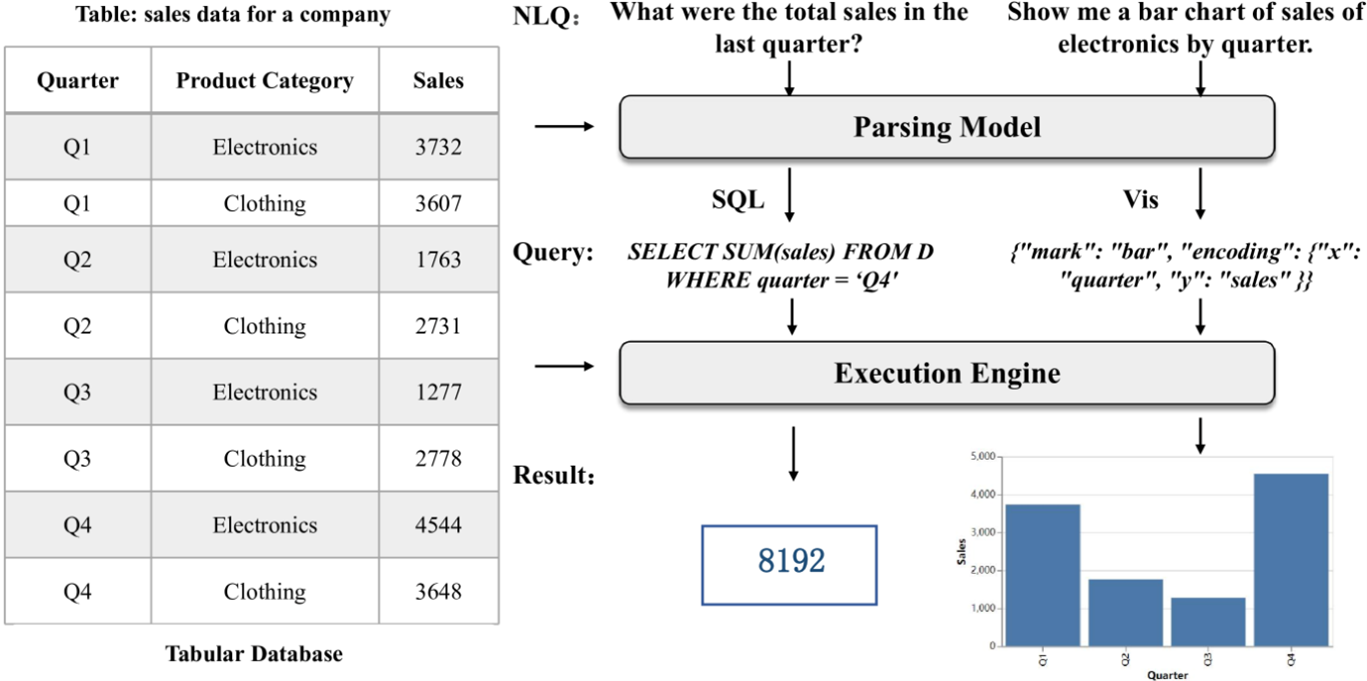
\includegraphics[width=6in]{Figures/NLQ.png} % ≤ 6 inches wide
    \caption[A general architecture of NLP models application in VA systems]{The application of natural language processing (NLP) for transforming commands in natural language into database SQL queries (on the left) and visual queries (on the right) in a visual analytics (VA) system (adopted directly from Zhang et al.~\cite{zhang2024natural})}
    \label{NLQ}
\end{figure}
\begin{figure}
    \centering
    % Ensure figure width fits within SFU margins
    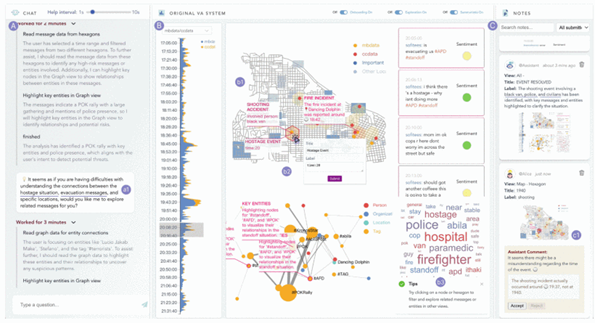
\includegraphics[width=6in]{Figures/LLMVA.png} % ≤ 6 inches wide
    \caption[Interaction and conversation between user and LLM agent in a VA system]{\textit{ProactiveVA}'s interface: The user can ask questions about the visualization in the chat panel on the left (A), and the LLM agent provides responses and its reasoning process based on the user’s prompt in the same conversation panel. The LLM agent is also able to highlight some parts of the visualization (b1) to direct the user’s attention towards specific parts of the visualization. The findings of both the user and the agent are also stored for later review and summarization and shown in the panel on the right (C) (adopted directly from Zhao et al.~\cite{zhao2025proactiveva})}
    \label{LLMVA}
\end{figure}
In a system like the one shown in Figure ~\ref{NLQ}, the embedded NLP model parses the user’s natural language query (NLQ) into either a structured query language (SQL) that is executable by the database or a JSON-like visual query that specifies both the structure of the chart and the data to be visualized on the UI client side. Such a system can particularly be employed in the VA-based intelligence workflow for visualization specification, which in turn facilitates hypothesis generation by the user.\par
Over a specified visualization, the \textbf{hypothesis and insight generation} can also be boosted by the interaction between the user and an embedded LLM. The reasoning power of LLMs can assist the user in the generation of narratives and plausible explanations for observed trends. When integrated with VA systems, LLMs act as cognitive amplifiers, bridging the gap between raw data, ML outputs, and human understanding. Figure ~\ref{LLMVA} provides an example of a VA system (from Zhao et al.~\cite{zhao2025proactiveva}) that utilizes an LLM chatbot agent for enhancing the user’s understanding of the visualized data via chat-based interaction. In an interface like the one shown in Figure ~\ref{LLMVA}, the user can ask questions about the different aspects of the visualization in the chat panel on the left (A), and the LLM agent responds to the user's prompt in natural language. The agent is also able to highlight some parts of the visualization (b1) to direct the user’s attention towards hidden patterns in the visualized data for augmented sense-making. The user can also add custom annotations (b2) and access onboarding tips (b3) for guidance. (C) Notes View stores both the user's and agent's findings for review and summarization. The agent can also validate the user's notes (c1) to improve the accuracy of the user's generated insights.\par 

Lastly, VA systems rely on NLP for \textbf{preprocessing unstructured data} towards building a visualizable model of the topics in the data. The NLP models for this purpose may either be dependent on ML algorithms for classification or clustering of the topics in the unstructured source or work based on experts’ predefined rules and symbols. While an example of the former was shown previously in Figure ~\ref{TimeSets}, Demelo and Sedig~\cite{demelo2021interfaces} have proposed a VA system (i.e., \textit{VisualQUEST}) that primarily relies on expert-defined ontologies for mediation of knowledge resources to expand and align user queries with domain vocabulary, thereby enhancing search precision and facilitating effective triage of large document collections.

\subsection{Existing Researches on the Application of Data-Driven Tools for Decision Design Stage} \label{ExistingResearchDesign}
Data-driven tools and techniques are applied primarily in the Design stage of the generic decision-making process to generate a set of criteria, alternatives, environmental factors, and the logical relationships between all of these \textit{variables}, so that the effect of selecting any alternative on all the criteria becomes measurable. For this, DM’s prior knowledge and expertise on the subject matter are crucial for specifying the causal dependencies between plausible courses of action taken, uncontrollable variables, and the outcomes achieved upon interventions. In addition, referring to Figure ~\ref{DDTAssignment}, we observe that data visualization (VIZ), machine learning (ML), traditional statistics (TS), and natural language models (NLMs) are also key tool families that support the activities of the Design stage. Therefore, a process model framework (similar to visual analytics for Intelligence) is needed in the Design stage as well to describe the flow of activities in this stage by taking the subject matter expert (SME)'s \textit{causal knowledge} into account and provide the foundation for later orchestration and integration of the above DDTs.
\subsubsection{Causal Graph Construction Process}
For complex decisions involving numerous interdependent variables, feedback mechanisms, and uncertain outcomes, building a causal graph is essential because it makes the underlying cause-and-effect structure of the problem explicit. Causal graphs help decision-makers identify key drivers, distinguish genuine causal relationships from mere correlations, recognize confounding factors, and evaluate the potential consequences of interventions before implementation. By providing a transparent representation of how variables influence one another, causal graphs support more robust reasoning, counterfactual analysis, and explainable decision-making in complex systems. Research has shown that (directed) causal graphs improve the design and interpretation of decision-analytic models by clarifying causal assumptions and dependencies, particularly as problem complexity increases, while causal models more broadly enable decision-makers to explain why specific actions are expected to produce desired outcomes and what trade-offs or risks they entail ~\cite{cox2021information,dijk2025directed}.\par
Kling~\cite{kling2025co} has proposed a process model for interactively constructing and validating causal graphs, which we can use for eliciting the orchestration and integration of data-driven tools in the context of decision-design-oriented causal reasoning. This interactive process of co-developing causal graphs involves the following steps:\par
\textbf{1. Problem Definition:} SME identifies the outcomes of interest and decisions that are likely to affect the outcomes, and candidate causal factors.\par
\textbf{2. Initial Causal Graph Construction:} SME and statistical modeler (SM) propose directed causal relationships. SME assigns belief scores (0–3) to every causal relationship.\par
\textbf{3. Data Collection and Preparation:} SM collects and preprocesses the observed data. An initial exploratory analysis and descriptive statistics are performed on the organized data.\par
\textbf{4. SCM Fitting:} A \textit{structural causal model (SCM)} is fitted for every dependent (\textit{child}) variable node in the initial graph. A basic SCM can be a linear regression equation with an intercept and noise.\par 
\textbf{5. Statistical Testing:} A raw p-value is derived for every causal relationship by performing a t-test on its \textit{edge coefficient}. SCM-induced covariances might also be estimated and compared with those of the observed data for model validation.\par
\textbf{6. Adjustment of the P-values:} A Benjamini-Hochberg (BH) procedure is applied to revise every edge's raw p-value by taking its pre-assigned causal strength (in step 2) into account.\par
\textbf{7. Visual Feedback and Collaborative Review:} An updated version of the causal graph with directed arrows, parameter estimates (edge coefficients), and adjusted p-values is visualized, and non-significant causal links are highlighted. SME + SM examine unsupported links and covariance mismatches.\par
\textbf{8. Iterative Refinement Loop:} Add/remove edges, revise beliefs, and refit SCM.\par
In this process, a methodological compromise between the SME's causal knowledge (belief) and the observed data is made by the introduction of \textit{false discovery cost rate (FDCR)} measure—an extension to \textit{false discovery rate (FDR)}—which takes the SME's belief scores into account as the costs of rejecting the hypothesized causal relationships. As every edge coefficient's raw p-value is calculated purely based on the observed data, it should be adjusted in a way that reflects the SME's level of certainty about the existence of a causal relationship between the parent and child nodes of its corresponding edge in the graph, for deciding whether it should be kept in the causal graph. The higher the certainty about a causal relationship, the harder it becomes for the procedure to reject it despite not being supported by the observed data. Figure ~\ref{CausalConstruction} illustrates the above causal graph construction process over an example case from Kling~\cite{kling2025co}.\par
\begin{figure}
    \centering
    % Ensure figure width fits within SFU margins
    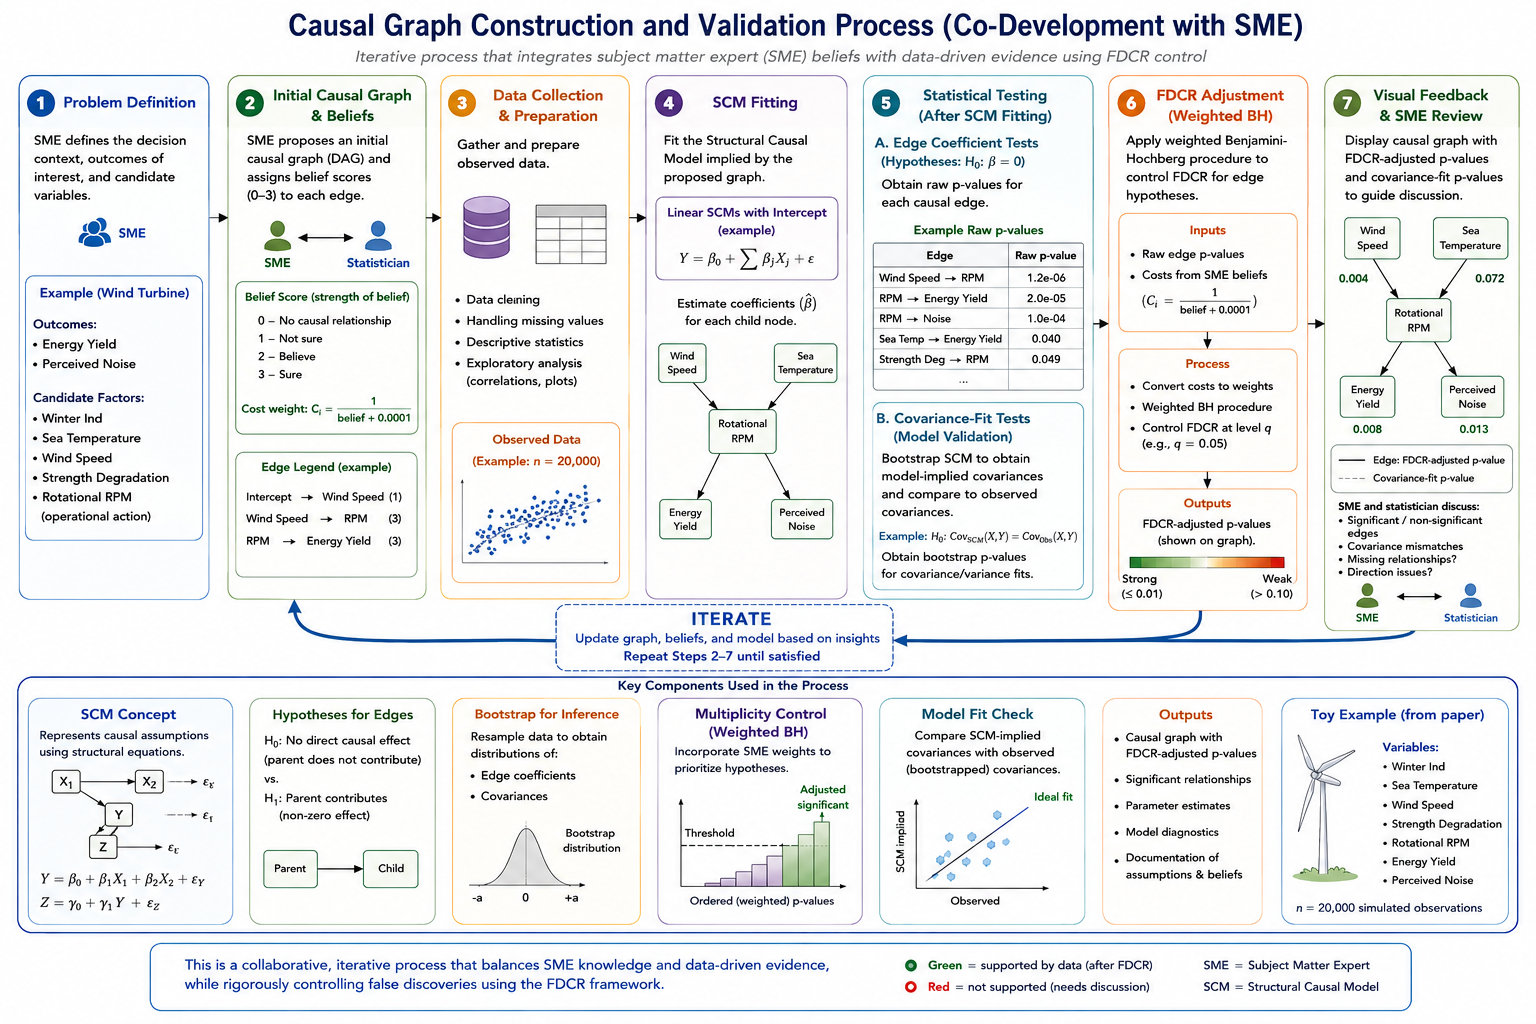
\includegraphics[width=6in]{Figures/CausalGraphConstructionProcess.png} % ≤ 6 inches wide
    \caption[A human-and-data-centered process of causal graph construction]{A human-and-data-centered interactive process for causal graph construction, implemented for an example case of deriving causal factors involved in prediction and estimation of wind turbines' energy yield and perceived noise (adopted from Kling~\cite{kling2025co}, and re-built using gen-AI).}
    \label{CausalConstruction}
\end{figure}
\subsubsection{Causal Graph Types}
While a causal graph construction process like the one proposed by Kling~\cite{kling2025co} can bridge the gap between data analytics and DM's causal knowledge, it does not delve into the specifics of the causal graph developed over the iterative process. In general, transforming structured data into a visual network (e.g., causal graphs) in which the variables are represented by nodes and the relationships are encoded by edges facilitates navigating the entire network's topography for viewers, as they do not have to over-rely on their working memory to track the variables and their interdependencies ~\cite{munzner_visualization_2015}.
Not surprisingly, we observe that researchers in diverse fields have used graphs and networks to visualize causal links and factors related to their study domain. We hereby shed light on multiple variations of these visual graph models that have commonly been adopted in different research areas and investigate how each of them suits a specific context of a decision problem in a practical setting. The familiarity with the particular use-cases of these visual models of cause-and-effect representation can assist designers with conducting an informed tool \textit{selection} and \textit{customization} from the VIZ DDT class of tools and techniques relevant to the design stage.\par
\noindent \textit{\textbf{Directed Acyclic Graphs}}\par
Directed acyclic graphs (DAGs) are the simplest type of graph that visualizes the hypothesized causal relationships between the identified causal factors in a particular context. Despite being very simple, they are very effective intuitive tools for pinpointing the existence of confounding variables in human systems and for spotting biases in perceived causal relationships ~\cite{shrier_reducing_2008,williams_directed_2018,digitale_tutorial_2022}. Figure ~\ref{DAGExample} demonstrates an example of a DAG that has been taken from Williams et al.\cite{williams_directed_2018}, visualizing how \textit{parental education} hypothetically causes \textit{self-harm} through other variables such as \textit{screen time} and \textit{obesity}. In this example, the effect of \textit{screen time} on \textit{obesity} is mediated by \textit{physical activity}, while confounded by \textit{parental education}. Both \textit{screen time} and \textit{obesity} variables collide in \textit{self-harm}, which is directly caused by both \textit{screen time} and \textit{obesity}.\par 
\begin{figure}
    \centering
    % Ensure figure width fits within SFU margins
    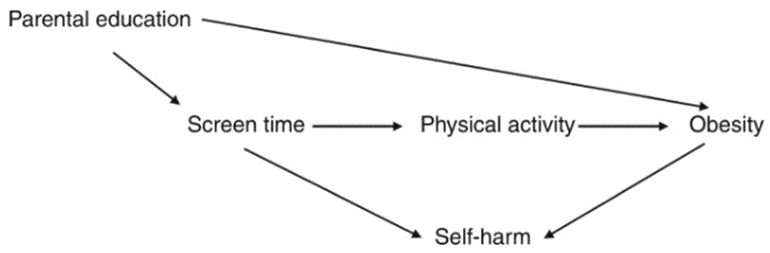
\includegraphics[width=6in]{Figures/DAGExample.png} % ≤ 6 inches wide
    \caption[A directed acyclic causal graph example]{A directed acyclic graph (DAG) visualizing how the effect of screen time on obesity is mediated by a child's physical activity, while confounded by parental education. Both screen time and obesity variables collide at self-harm (adopted directly from Williams et al.~\cite{williams_directed_2018}).}
    \label{DAGExample}
\end{figure}
In DAGs, all decision variables, regardless of their type (outcome, lever, etc.), are encoded as graph nodes, and the causal relationship between any two variables is encoded by a directed arrow from the cause (parent node) to the effect (child node). DAGs are acyclic in the sense that no closed loop can be found in any part of the graph, as no variable can cause itself directly or indirectly in a certain snapshot of time. Although instantaneous in DAGs, some other types of causal network (e.g., causal loop diagrams) capture causal interactions over a period of time, allowing \textit{loops} to form in their graph structure.\par
While simple DAGs without extra visual encodings are effective tools for externally representing DMs’ perceived causal relationships between decision variables, they are sometimes equipped with elements such as numbers, annotations or mathematical formulas at their nodes and/or their links to represent information such as the current state/value of variables or relationships’ strength, certainty, or mapping functions. In Figure ~\ref{AnnotatedDAG}, a directed causal graph from Montibeller and Belton~\cite{montibeller_causal_2006} has been illustrated in which the strength of the causal links has been annotated by both qualitative (a) and quantitative (b) scales. The plus (+) sign near the head of the arrows denotes the positive direction of the causal relationship, meaning any amplification of the variable as the cause results in the amplification of the variable as the effect.\par
\begin{figure}
    \centering
    % Ensure figure width fits within SFU margins
    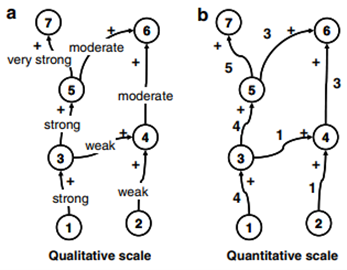
\includegraphics[width=4in]{Figures/AnnotatedDAG.png} % ≤ 6 inches wide
    \caption[An annotated directed acyclic causal graph example]{Use of words, numbers, and icons to communicate the strength and polarity of the causal relationships in a DAG. In (a), the relationship strengths have been denoted by a qualitative scale that uses ordinal values such as weak, moderate, and strong. In (b), the relationship strengths have been shown by a quantitative scale of numbers from 1 (very weak) to 5 (very strong). The plus (+) sign on the links’ arrows means the positive polarity (direction) between the source variable and the destination (adopted directly from Montibeller and Belton~\cite{montibeller_causal_2006}).}
    \label{AnnotatedDAG}
\end{figure}
One particular type of annotation applied to the edges of acyclic graphs refers to the probability of occurrence of the target phenomenon, given that the source phenomenon occurs. This type of annotation is mainly seen on \textit{causal Bayesian networks (CBNs)}. The simplest type of CBN is the one in which the variables come in specific hierarchies forming \textit{probability trees}. We have illustrated a tree denoting the probabilities for multiple states of each thermodynamic property of water inside an Internet of Things (IoT) sensor in a hierarchical structure in Figure ~\ref{IoTBayesianNetwork}, adopted from Bradford et al.~\cite{bradford_knowledge_2020}.\par
\begin{figure}
    \centering
    % Ensure figure width fits within SFU margins
    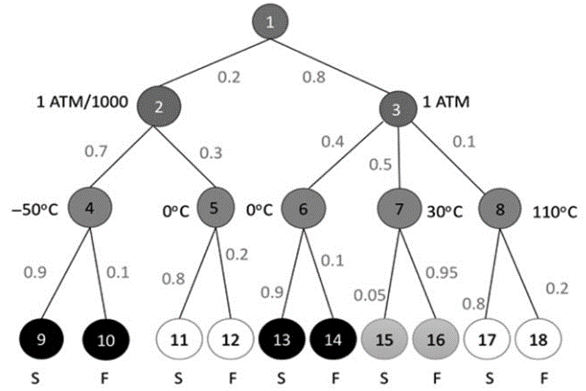
\includegraphics[width=5in]{Figures/BayesianNetwork.png} % ≤ 6 inches wide
    \caption[A Bayesian probability tree example]{A probability tree for an IoT sensor recording different states of multiple thermodynamic characteristics of water. The very first level of the tree hierarchy after the parent node retains the possible states of pressure, the second level shows the possible values for the water temperature, and the last level holds the water phases information. The probability for a specific state of a property to result in a lower-level property has been denoted beside the links that connect a state of a property to a state of the lower-level property (adopted directly from Bradford et al.~\cite{bradford_knowledge_2020}).}
    \label{IoTBayesianNetwork}
\end{figure}
\noindent \textit{\textbf{Directed Cyclic Graphs (Causal Loop Diagrams)}}\par
The most important assumption when drawing a DAG to visualize the cause-and-effect relationships between decision variables is that the formation of any causal loop is not allowed. This rule in DAGs ensures that no self-causation paradox takes place in which a variable becomes a cause of its own existence at a specific point in time ~\cite{byeon2023directed,feeney2025use}. However, there are cases in which the current state of a variable can directly or indirectly affect its future state. An example of such a situation has been demonstrated in Figure ~\ref{CLDFishing} from Banitz et al.~\cite{banitz_visualization_2022}, in which variables such as fish population, mortality, and reproduction have been considered to be indirectly and inclusively caused by themselves in a causal structure, called a \textit{causal loop diagram (CLD)}.\par
\begin{figure}
    \centering
    % Ensure figure width fits within SFU margins
    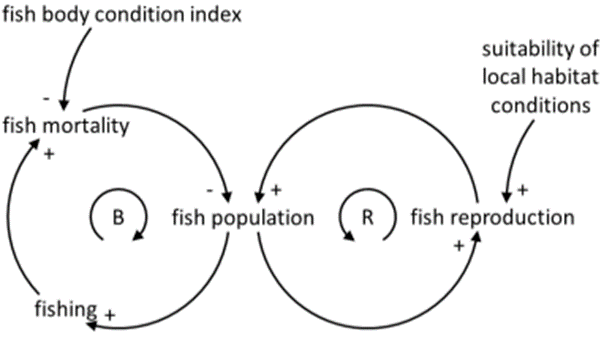
\includegraphics[width=5in]{Figures/CLDFishing.png} % ≤ 6 inches wide
    \caption[A Bayesian probability tree example]{A causal loop diagram (CLD) visualizing the causal relations between fish population, reproduction, mortality, and fishing rate. Two directed loops have formed and labeled as B (balancing) and R (reinforcing) to demonstrate how a change in a variable inside each loop would cause a subsequent change in the same variable’s value, while positive (+) and negative (-) signs on the arrowheads show the polarity of the causal relationships between every pair of cause and effect variables (adopted directly from Banitz et al.~\cite{banitz_visualization_2022}).}
    \label{CLDFishing}
\end{figure}
In addition to arrows and polarity signs (which are also occasionally present in DAGs), many CLDs include a notation to visualize the polarity of the formed causal loops in different ways. The one that is very common and also seen in Figure ~\ref{CLDFishing} involves using letter R or B enclosed by a circular arrow in the middle of the formed loops, representing whether the causal loop is either \textit{reinforcing} or \textit{balancing}. The reinforcing loops are those in which a change in the current state of a variable in the loop will eventually cause a change in the future state of the same variable in the same direction as the initial change. In Figure ~\ref{CLDFishing} example, the loop formed between \textit{fish population} and \textit{fish reproduction} is reinforcing, as the increase in the value of any variable inside that particular loop will result in an increase of the same variable’s value in the future (e.g., if \textit{fish reproduction} increases, \textit{fish population} will increase, making the \textit{fish reproduction} increase again in the future). On the other hand, in a balancing loop like the one between fish population and mortality, an increase in a variable’s current value will result in a decrease in the same variable’s future value, and vice versa. In many created CLDs in research of different disciplines, visual elements such as icons and color channels are employed to better differentiate between the polarity of causal relationships and loops. The important note in the interpretation of CLDs is that the self-causations are all indirect and time-delayed, meaning that the feedback of a change in a variable’s value inside a loop is necessarily reflected via other variables in the same causal loop and over time. This is the reason why CLDs are an integral tool in the field of \textit{System Dynamics (SD)}.\par
\noindent \textit{\textbf{Stock Flow Diagrams}}\par
Another visual representation of the time-variant causal relationships is \textit{stock-flow diagram (SFD)}. Being intensively used in SD modeling, SFDs go deeper than CLDs in the specification of time-delayed causal mechanisms by visually differentiating between the \textit{stock} variables and \textit{rate (flow)} variables. Stock variables are the variables that possess a certain and measurable value at any given time. In Figure ~\ref{CLDFishing} example, the fish population is a stock variable, as its value is measurable at any point in time. On the other hand, rate variables’ value can only be measured in a given time frame. Fish reproduction, mortality, and fishing are all rate variables in Figure ~\ref{CLDFishing} as they can only be measured in a period of time rather than at a certain point in time. The net accumulation of all the rate variables over time determines a stock variable’s value. In Figure ~\ref{SFDPocketMoney}, a SFD visualizing the dynamic causal relationships between the different variables involved in a perceived model of a child’s pocket money has been represented from Binder et al.~\cite{binder2004developing}.\par
\begin{figure}
    \centering
    % Ensure figure width fits within SFU margins
    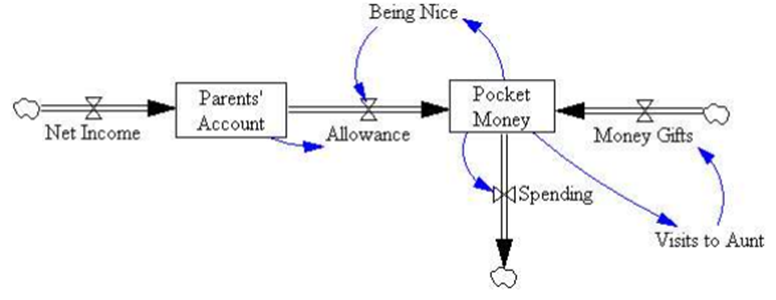
\includegraphics[width=6in]{Figures/SFDPocketMoney.png} % ≤ 6 inches wide
    \caption[A stock-flow diagram (SFD) example]{A stock-flow diagram (SFD) demonstrating the causal relationships between the variables for a child's pocket money example. Stock variables have been demonstrated with rectangular boxes where materials (in this case, money) are accumulated, and the valve icons over the middle of black arrows visualize the rate variables, which cause the values of the stocks to change. The rest of the variables are auxiliary variables that complete the information flow (adopted directly from Binder et al.~\cite{binder2004developing}).}
    \label{SFDPocketMoney}
\end{figure}
As we can see in the SFD visual model in Figure ~\ref{SFDPocketMoney}, the rate variables, including \textit{net income}, \textit{allowance}, \textit{money gifts}, and \textit{spending}, have all been visualized by a valve icon overtop of a directed arrow showing the flow direction in or out of the variables inside the boxes. The variables inside the boxes are all stock variables, namely \textit{parents’ accounts} and \textit{pocket money}. The values of these stock variables are dependent on the value of those rate variables attached to them by the directed arrows. The variables like \textit{being nice} and \textit{visits to aunt} are the causal intermediates, hereby called \textit{auxiliary} variables, realizing the flow of information between the variables of different types. The enclosed cloud-shaped icons connected to the ends of the rates represent the flow of the material (in this case, money) going in/out of the system’s boundary. The informational causal relationships have also been noted by the blue arrows. Such elaborate visual notations set the basis for quantitative specifications of how a dependent variable’s value is derived from its independent variables in a model. The quantification of the causal relationships, however, is pervasively done with the aid of computer programs. Multiple software applications (e.g., Vensim, AnyLogic, Stella, and Simantics) have made the creation and quantification of SFD visual models possible.\par

\noindent \textit{\textbf{Causal Decision Diagrams}}\par
First introduced by Pratt~\cite{pratt_link_2019}, a \textit{causal decision diagram (CDD)} is a visual model that helps decision stakeholders capture their perception of how taking a set of \textit{actions} leads to a set of \textit{outcomes} through a sequence of causal chains. CDDs’ visual marks are fairly similar to DAGs, except that CDDs exploit additional encodings to differentiate between different types of variables, making them more decision-oriented compared to the other causal networks. Variables in a CDD are either Outcomes which the progress towards decision goals are measured with, actions which DMs have control over their values, \textit{externals} which are exogenous to the system and DMs do not have control over their value, and \textit{intermediates} that complete the chain of causality from actions and externals to outcomes ~\cite{pratt_link_2019,pratt_bringing_2023,pratt_decision_2023}. An example of CDD has been illustrated in Figure ~\ref{CDDNematode} for a decision on what crop to plant and what type of nematicide to use in the next two years for an agricultural field to maximize its total biennial profit.\par
\begin{figure}
    \centering
    % Ensure figure width fits within SFU margins
    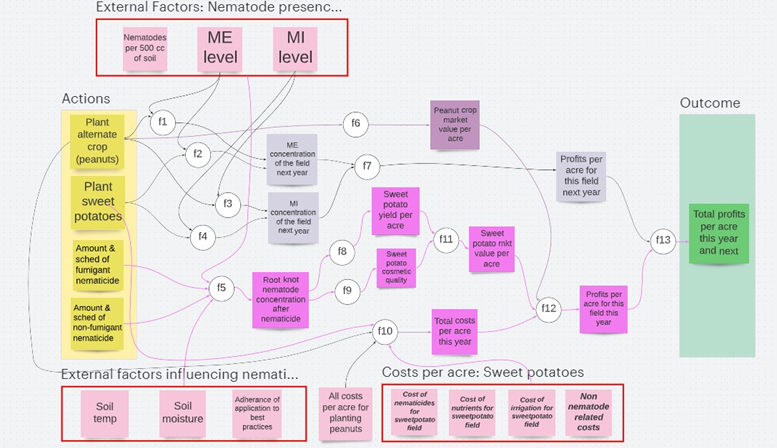
\includegraphics[width=6in]{Figures/CDDNematodes.png} % ≤ 6 inches wide
    \caption[A CDD example]{A causal decision diagram visualizing causal relationships between action, external, intermediate, and outcome variables for a decision on what crop and nematicide type to use in a sweet potato field to maximize its profit per acre in the next two years (taken from the SharePoint repository of the DECIDE-SMARTER grant project, with permission).}
    \label{CDDNematode}
\end{figure}
Differentiated by the background color of yellow in Figure ~\ref{CDDNematode}, the nodes for action variables have been grouped and placed on the left side of the graph. The actions that DMs in this example can take are to plant sweet potato, plant peanuts as the alternate crop, amount of fumigant and non-fumigant nematicide to use for the next two years. Both on top and bottom of the graph, nodes of external variables have been placed and include every factor that is affecting the causal mechanism of how actions lead to outcomes, yet is out of DM’s control. Factors like current nematodes’ presence level, soil temperature and moisture, and different costs regarding planting and nematicide are all external to this decision problem. At the very right side of the graph, we also observe a single node representing the only identified outcome variable, which is the farm’s total profit per acre after two years. In the middle of the graph, several colored sticky nodes are visible that represent the intermediate variables that complete the causal chain of actions to outcomes. The annotated white circles before the intermediate and outcome variables denote the presence of mathematical functions that determine the value of each of these dependent variables from the values of their independent variables. The existence of intermediates along with the causal links (which are shown by the directed lines) between them provides transparency and explanatory analysis of DMs’ perception of the real world’s causal interactions involved in a complex decision problem. As the visual space of CDDs involves the same visual marks of DAGs in a grouped structure to comply with decision problems' semantics, we consider CDDs as the representative of all different variations of directed acyclic graphs by default.\par
\noindent \textbf{Summary Analysis of Causal Graph Types for Decision Design}\par
Considering CDDs, CLDs, and SFDs as the main options for specifying the relationships between the different decision variables, a DM can employ and customize either of these visual toolkits according to the decision problem’s level of complexity, decision and variable types, and the user’s personal characteristics. To derive the information on when and how to use each of the above causal graph types, we refer to the existing research literature related to the causal graphical models from task-related, data-related, and user-related viewpoints.\par
We inferred from the literature that both CLDs and SFDs—as SD tools for visually modeling causality—are capable of visualizing feedback loops as an integral part of the dynamic systems’ theory, a capability that DAGs do not possess. Therefore, DAGs are ruled out when DMs need to visualize feedback mechanisms between a set of decision variables. Aiming to qualitatively analyze the causal relationships between the variables and communicate on the involved factors while the feedback loops are present, cyclic graphs like CLDs are popular choices because of their relative simplicity and ease of creation. If a quantitative analysis of the decision variables and scenarios is needed while feedback loops exist in the system’s model, the use of SFDs becomes justified. Formal SFD modeling, however, involves a set of relatively complex visual jargon, making these models sometimes too difficult to be understood by the decision stakeholders (especially the novice ones) with minimal training and effort, eventually causing extra cognitive load on their working memory. Any of these visual networks can also be customized with various visual elements, marks, and channels for different purposes. From multiple research studies done, it is inferred that adding extra features in terms of textual annotations and color highlighting improves perception and learning from visualized data for users with lower prior knowledge levels. On the other hand, adding the same features imposes an extra cognitive load on users with a high prior knowledge level by interrupting their natural flow of thinking, making a negative impact on their learning from visualization ~\cite{han2023prior}. Even for novices, the application of too many elements and the absence of grouping patterns for related items result in visual cluttering and cognitive overload. For causal relations in particular, the application of animated visual elements (such that a shape moves out of a cause node and hits the effect node) in a causal network enhances users’ ability to memorize and recall the causal semantics ~\cite{kadaba_visualizing_2007}.\par
Existing computer programs that provide causal modeling capability in terms of visual networks offer a variety of features for customizing the created network elements. As a result, a decision maker or modeler can establish hybrid visual models that bring in properties of different causal models together if necessary. One such property is the measurability of causal relationships’ strength, which is the step after the relationships’ identification and specification. However, many of these tools only support ideation and elicitation of causal dependencies and not their quantification and measurement (which normally happens after the specification of causal relationships). Miro, Lucidchart, and FigJam are examples of these ideation and diagramming applications, providing tools that decision stakeholders can use to build externalized causal networks. Despite being powerful in graphical modeling, the named applications fall short when it comes to computing quantities in a created causal model. System dynamics software applications(e.g., Vensim) go beyond the visual modeling of causal interactions and provide formula-writing and scenario analysis capabilities.
\subsubsection{LLM-aided Generation of Causal Variables}
Recent research has begun to augment LLMs with explicit causal reasoning capabilities to improve their applicability in complex decision-making tasks. For example, Chen et al.~\cite{chen2025causal} proposed a learning–adapting–acting framework in which an LLM collaborates with an SCM to iteratively acquire, refine and exploit causal knowledge explicitly, rather than relying solely on the implicit knowledge encoded in pretrained language models. During the learning stage, the LLM analyzes textual descriptions of the environment to identify domain-specific causal entities and infer causal relationships among them, thereby constructing an initial causal graph represented as an SCM. The adapting stage subsequently updates this causal graph through feedback obtained from environmental interactions and causal interventions, enabling the model to revise inaccurate or incomplete causal assumptions. Finally, in the acting stage, the refined SCM guides a reinforcement learning agent in selecting more effective actions, allowing decision-making to be grounded in an explicitly represented causal understanding of the environment rather than purely statistical correlations. Experimental evaluation across multiple open-world decision tasks demonstrated that integrating LLMs with causal modeling substantially improves policy learning and decision quality compared with conventional LLM-based approaches.

A complementary line of research focuses specifically on employing LLMs to construct causal graphs from unstructured textual information. Li et al.~\cite{li2025beyond} presented a hybrid framework that combines LLM reasoning with linguistically informed feature engineering to generate high-quality causal graphs from narrative documents. The workflow begins by prompting an LLM to summarize lengthy narratives into concise, agent-centered events and factors that serve as candidate causal nodes. Instead of relying exclusively on the LLM for causal reasoning, the framework subsequently incorporates a linguistically motivated "Expert Index" together with a situation–task–action–consequence (STAC) classification model to identify plausible causal links among the extracted entities. Finally, an iterative prompting strategy progressively refines the graph by validating, expanding, and connecting the discovered relationships into a coherent causal structure. Experimental comparisons with GPT-4o and Claude 3.5 showed that this hybrid methodology produces more accurate, interpretable, and structurally coherent causal graphs, demonstrating that LLMs are particularly effective for identifying causal factors and proposing initial graph structures when complemented by additional linguistic reasoning mechanisms.

Collectively, these studies demonstrate an emerging role for LLMs in supporting the early stages of causal decision modeling. Rather than replacing established causal discovery or optimization methods, LLMs primarily contribute by extracting decision-relevant concepts from natural-language knowledge, generating candidate causal variables, proposing initial causal relationships, and constructing preliminary causal graphs that can subsequently be refined through computational causal analysis, intervention data, or expert feedback. These capabilities suggest that LLMs can substantially reduce the manual effort required for knowledge elicitation and model initialization while maintaining the human expert in the loop for validation and refinement.
\subsubsection{Validation and Measurement of Causal Relationships}
Measurement of causal relationships involves deriving functions that map the values of independent variables to the values of dependent ones in a causal model. This step is crucial for both verifying the causal assumptions made in the previous (causal relationship specification) step and determining the values of decision criteria upon choosing every decision alternative. According to Pearl~\cite{pearl_causal_2009}, probabilistic relationships between the variables could be the result of causation, confounding, or selection bias. Therefore, no strict conclusion could be made yet about the existence of causal interaction between two variables when a statistical association is found from pure observation. If decision stakeholders want to verify a presumed causal relationship, an intervention on the assumed cause (in addition to fixing the state of other variables) is needed to check whether the value or the probability of a specific value for the effect variable changes. In formal terms, if X and Y are respectively the assumed cause and effect variables, then the causal claim is supported if:
\begin{equation}
    P(Y\mid do(X=x_1 ) )\neq P(Y\mid do(X=x_0 ))
\end{equation}
Which $x_0$ and $x_1$ are two different values of the cause variable $X$ that are set by the human’s direct intervention and formalized by do-calculus notation. In terms of structural equation models (SEMs), the above probabilistic formulation turns into a deterministic function $f$ as:  
\begin{equation}
    f_Y (x_1,U_Y)\neq f_Y (x_0,U_Y))
\end{equation}
In which $f_Y (x_i,U_Y)$ denotes the value of Y as a causal function of $X=x_i$ when $U_Y$ is an exogenous disturbance exposed to the causal relationship between X and Y. However, this randomized intervention does not guarantee the existence of a direct causal relationship but rather falsifies an assumed causal relationship that is not supported by observational data.\par
In scenarios where intervention is not possible, the decision-maker has to rely primarily on observational data to test a causal assumption. To make a causal inference from observational data, contingency tables that denote the conditional probabilities of the effect variable given certain values for every cause are widely used. Contingency tables can be either purely textual or contain visualized data. In Figure ~\ref{ContingencyTables}, three different forms of a contingency table denote the conditional probabilities that a disease occurs in several subjects given that a recessive gene exists in their body or not, and treatment is performed on them or not. Kale et al.~\cite{kale_causal_2022} found that the visualization of conditional probabilities (such as those of cases B and C in Figure ~\ref{ContingencyTables}) does not reliably improve the causal inference ability of users, while it leads to the users’ insensitivity to the population’s sample size.\par
\begin{figure}
    \centering
    % Ensure figure width fits within SFU margins
    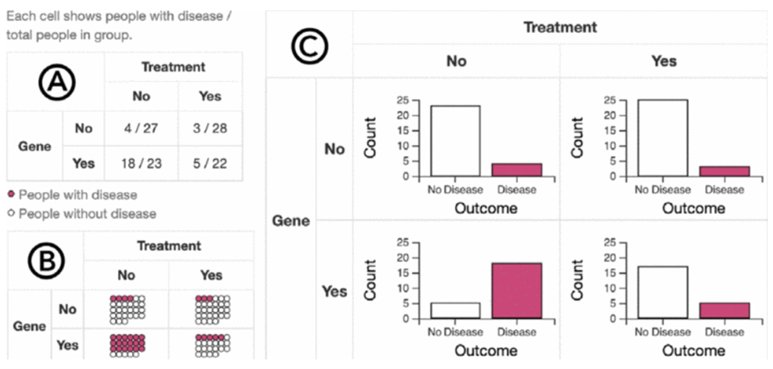
\includegraphics[width=6in]{Figures/ContingencyTables.png} % ≤ 6 inches wide
    \caption[Different forms of contingency tables]{Different forms of contingency tables to demonstrate the conditional probabilities for a group of people to be diagnosed as diseased given a recessive gene is either present or not, and treatment is done or not. In (A), the conditional probabilities data are purely textual. In (B), conditional probabilities are presented in the form of faceted icon arrays. In (C), faceted bar graphs visualize the number of people with disease or no disease for each condition (adopted directly from Kale et al.~\cite{kale_causal_2022}).}
    \label{ContingencyTables}
\end{figure}
In addition to contingency tables, 2D visualization of the data of believed cause-and-effect variables might also be used to informally verify a causal dependence. According to Wang et al.~\cite{wang_causal_2025}, users’ perception of the existence of a causal relationship between two variables from a visualization is dependent on their prior belief of the existence of such causation, the level of visualized association of the data from both variables, and the type of visualization itself. For lower levels of visualized associations, scatterplots induce a stronger sense of the existence of a causal relationship between variables, while bar graphs create the same perception in users when the visualized association between the variables’ data is higher ~\cite{wang_causal_2025}. A stronger or weaker causal relationship is also inferred when the discrepancy between the visualized association and the causal prior of users becomes increasingly positive or negative in order. However, the confidence of users in their perceived causal relationship only increases significantly when the visualized association level between the variables’ data is higher than what they had already perceived and is not susceptible to decrease when the visualized association level is lower than their prior perception of the strength of the causal relationship ~\cite{wang_causal_2025}.\par
To be usable for measuring the outcomes achieved after taking different courses of action, it is required to estimate the structural function for each dependent variable within a verified causal model of the consensus of SMEs and decision stakeholders. Considering the causal inferences are beyond the pure observational data and come from the mechanisms through which the real-world phenomena take place, specification and measurement of causal relationships both need human experts' supervision and involvement to inform the causal model with their formal and tacit knowledge of the subject matter. Findings from recent empirical studies also suggest that the knowledge of subject matter, despite the application of automated causal discovery tools, is still important for algorithm selection, parameter tuning, and confounder adjustment ~\cite{gururaghavendran_can_2025}.\par
As pointed out earlier in the causal graph co-construction process from Kling~\cite{kling2025co}, SMEs inform the causal models with SCMs —most notably \textbf{linear regression models (LRMs)}— that best describe the causal relationships between a dependent variable and its independent variables within the context of the literature of the subject matter. In general, the predictive ML models (e.g., LRM) are mainly adopted when decision stakeholders and SMEs believe to some extent that there is a causal relationship between a target variable and the source(s), while no clear function is known to estimate the value of the effect variable from the cause(s) ~\cite{renero_rex_2026}.\par
When the variable as the effect takes continuous numerical values, a simple LRM can be fitted for predicting its value from the values or states of its parents (causes). In formal terms, if $X_1$, $X_2$, to $X_n$ represent the values of independent variables (predictors) for the continuous dependent variable $Y$, then the estimated value of $Y$ ($\hat{Y}$) is predicted as:
\begin{equation}
    \hat{Y}=\beta_0 + \beta_1 X_1 + \beta_2 X_2 +\dots+ \beta_n X_n
\end{equation}
While $\beta_0$ to $\beta_n$ are regression coefficients and are calculated as follows:
\begin{equation}
    \beta_i=\frac{Cov(X_i,Y)}{Var(X_i)}
\end{equation}
While the values of other predictors ($X_{j\neq i}$) remain unchanged. The regression intercept ($\beta_0$) is also calculated as:
\begin{equation}
    \beta_0=\bar{Y} - (\beta_1 \bar{X_1} + \beta_2 \bar{X_2} +\dots+ \beta_n \bar{X_n})
\end{equation}
The fitness of such a linear function to explain the variability inside the data is also measured in terms of R-squared and adjusted R-squared. If these two measures are somewhere near zero, the decision-makers should double-check whether a linear function is a justified assumption for explaining the causal relationship between their variables of interest. The interaction effect of any number of the identified independent variables might also be considered, making the above relationship look like the following:
\begin{equation}
    \hat{Y}=\beta_0 + \beta_1 X_1 + \beta_2 X_2 +\dots+ \beta_n X_n + \beta_{ij}X_iX_j
\end{equation}
While $\beta_{ij}$ is the interaction coefficient between two different variables $X_i$ and $X_j$. The statistical significance of such a hypothetical interaction can also be tested as well using \textit{p-value} measure.\par
In the cases that the effect variable is of a categorical or binary type, a \textit{logistic regression model} can be derived to predict the probability of the dependent effect variable falling into a certain category given a certain set of values for the predictor variables are observed ~\cite{bender_ordinal_1997}. The following formalization models the logit of the odds for the dependent variable ($Y$) to fall into the $i^th$ category or any category before, as a linear function of the independent variables: 
\begin{equation}
    ln(\frac{P(Y\leq i)}{1-P(Y\leq i)})=\alpha_i + \beta_{i1} X_1 + \beta_{i2}X_2 +\dots+ \beta_{in}X_n
\end{equation}
In which $i$ is from 1 to $k$, $\alpha_i$ is the model’s intercept for the estimation of the odds value when the dependent variable falls into the first $i^{th}$ categories out of $k$ categories for $Y$, and $\beta_{i1}$ to $\beta_{in}$ are the regression coefficients of the $n$ independent variables for the estimation of the odds’ value for the dependent variable to fall into the first $i^{th}$ categories. In the \textit{proportional odds model (POM)}, these regression coefficients are assumed constant across all category cut-points, simplifying the above equation as follows ~\cite{brant1990assessing,mccullagh_regression_1980,armitage_proportionalodds_2005}:
\begin{equation}
    ln(\frac{P(Y\leq i)}{1-P(Y\leq i)})=\alpha_i + \beta_{1} X_1 + \beta_{2}X_2 +\dots+ \beta_{n}X_n
\end{equation}
Now, assuming that the odds of all categories are predicted with a constant set of regression coefficients, the probability of $Y$ falling exactly into the $i^{th}$ category is calculated as:
\begin{equation}
    P(Y=i)=P(Y\leq i)-P(Y\leq i-1)=\frac{e^{-\alpha_{i-1}}-e^{-\alpha_i}}{e^{z}+e^{-\alpha_{i-1}}+e^{-\alpha_i} + e^{-(z+\alpha_{i-1}+\alpha_i)}}
\end{equation}
In which $z=\sum_{r=1}^{n}\beta_rX_r=\beta^TX$ and $\alpha_{i-1}$ is the model’s intercept for the estimation of the odds value when the dependent variable falls into the first ${i-1}^{th}$ set of categories.\par
As seen, ML-aided model extraction is a data-intensive process and works best when the dataset’s volume is large. In-depth field observations and benchmarks are needed to derive further data for model training if the existing data is not sufficient for this purpose. Fortunately, many computer programs exist these days that can automate the process of extracting the coefficients of the hypothesized LRM. An open-source example of these programs is \textit{Scikit-learn (sklearn)}, a Python library that takes the data column of every variable as LRM's argument and returns an array containing the regression coefficients.\par
\begin{figure}
    \centering
    % Ensure figure width fits within SFU margins
    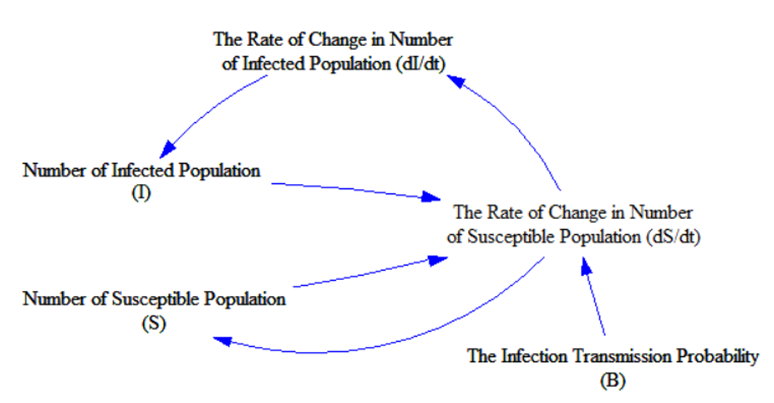
\includegraphics[width=6in]{Figures/CausalInfection.png} % ≤ 6 inches wide
    \caption[An example of cyclic causal graphs informed by non-linear SCM]{A cyclic causal graph visualizing the causal relationships between the rate of change in the number of people susceptible to being infected by a virus (e.g., COVID-19), the number of infected populations, the number of susceptible populations, and the rate of infection. The structural functions between every dependent variable and its independent variables in this model have already been directly taken from Kermack and McKendrick~\cite{kermack1927contribution} in classic epidemiology research.}
    \label{causalInfection}
\end{figure}
Last but not least, SME may inform a strongly believed causal relationship with a complex non-linear SCM derived directly from previous observations or conducted formal studies. For example, in the causal graph shown in Figure ~\ref{causalInfection} for investigating the impact of different variables on the spread of a virus (e.g., COVID-19) in the context of epidemiology, a non-linear function derived from Kermack and McKendrick~\cite{kermack1927contribution} is widely accepted and applied to estimate the rate of change in the number of susceptible people to the virus as follows:
\begin{equation}
    \frac{dS}{dt}=-\beta I S
\end{equation}
In which $\frac{dS}{dt}$ is the rate of change in the number of susceptible populations, $S$ is the current number of susceptible (and uninfected) people, $I$ represents the number of infected populations, and $\beta$ is the infection transmission probability.

\subsection{Existing Researches on the Application of Data-Driven Tools for Choice Stage} \label{ExistingResearchChoice}
DMs in the choice stage seek to evaluate all the options they have identified at the beginning of the design stage for dealing with the decision problem and select the one that most reliably satisfies all the decision criteria. As an approximate prediction of the outcomes of every possible alternative set of actions is crucial to weigh the options against each other, data simulation methods (SIM) and mathematical optimization models (MO) are extensively employed in this stage to assist DMs in finding/developing the optimal courses of action to take. Data visualization (VIZ), machine learning (ML) models, traditional statistics (TS) methods, and natural language models (NLM) can also be involved in facilitating the execution of different activities throughout the choice stage. Therefore, we investigate in-depth how recognized DDTs are and can be applied, customized, and integrated to support the evaluation and analysis of the outcomes of decision alternatives, according to various humanistic, data-relevant, and task-relevant factors. 
\subsubsection{Process Models for Choice Stage}
To identify appropriate opportunities for integrating data-driven tools within the choice stage, it is first necessary to examine the existing process frameworks that describe the sequence of activities typically undertaken during this stage. Such frameworks provide a conceptual roadmap for the systematic orchestration of data-driven techniques throughout the decision-making process. The literature presents several process models that characterize the activities involved in identifying and selecting an optimal solution from a set of feasible alternatives. These models have primarily been developed within the contexts of \textit{multi-criteria decision analysis (MCDA),} \textit{multi-objective optimization (MOO)},\textit{ robust decision-making (RDM)}, and \textit{sensitivity analysis (SA)}.\par
In the context of discrete multi-objective decision-making, Insua and French~\cite{insua1991framework} have proposed a framework in which sensitivity analysis has been treated as an integral component of the entire decision-making process, not only as a post-processing activity. They recommend that the following steps should be taken to select a sufficiently-robust alternative from a discrete set of solution after a decision problem is formulated:\par
\textbf{Step 1. Alternative Evaluation and Preference Modeling:} Each alternative is evaluated with respect to the identified criteria. The decision-maker's preferences are then represented using an appropriate multi-attribute value model or other preference model, allowing the overall desirability of each alternative to be assessed and an initial preferred solution to be identified.

\textbf{Step 2. Sensitivity Analysis:} The robustness of the preferred alternative is investigated by systematically varying uncertain model parameters, such as criteria weights, value functions, preference parameters, and performance estimates. The objective is to determine whether the recommended solution remains optimal under plausible changes in assumptions.

\textbf{Step 3. Model Revision and Iterative Refinement:} If the sensitivity analysis reveals that the recommendation is unstable, the decision-maker revises the preference model, acquires additional information, or modifies the set of alternatives. The evaluation and sensitivity analysis are then repeated until a sufficiently robust recommendation is obtained.

\textbf{Step 4. Final Decision Recommendation:} Once the preferred alternative demonstrates adequate robustness to uncertainty, it is recommended as the final decision, together with an understanding of the assumptions and conditions under which the recommendation remains valid.

In another integrated framework proposed by Belton~\cite{belton2002multiple}, MCDM has been viewed as an iterative learning and decision-support process rather than merely the application of a ranking algorithm. \textit{Problem structuring}—which is equivalent to \textit{problem formulation} in Insua and French~\cite{insua1991framework}, and occurs during the design stage of Simon's model—is followed by:\par
\textbf{Step 1. Preference Modeling:} Evaluation criteria are established, and the decision-maker's preferences are elicited using an appropriate MCDM methodology. This step develops the preference model that will be used to compare competing alternatives.

\textbf{Step 2. Alternative Evaluation:} The feasible alternatives are assessed against the established criteria using the selected MCDM technique. The resulting evaluations allow stakeholders to compare alternatives and understand the trade-offs among conflicting objectives.

\textbf{Step 3. Interactive Learning and Problem Refinement:} The evaluation results are reviewed collaboratively with stakeholders. Insights gained during the analysis may lead to refining objectives, modifying criteria, adjusting preference information, restructuring the problem, or generating additional alternatives. The evaluation process is repeated as necessary.

\textbf{Step 4. Sensitivity and Robustness Analysis:} Sensitivity analyses are performed to examine how changes in criteria weights, preference parameters, or uncertain input data influence the ranking or selection of alternatives. This step assesses the confidence that can be placed in the recommended solution.

\textbf{Step 5. Decision Recommendation and Implementation:} After confirming that the recommendation is sufficiently robust, the preferred alternative is selected for implementation. The framework also emphasizes reflecting on the decision process and incorporating lessons learned into future decision-making.

While the two frameworks discussed above emphasize the iterative and adaptive nature of identifying optimal solutions, they are both primarily concerned with selecting an alternative from a discrete set of candidate solutions. In many real-world decision problems, however, the decision space is continuous, resulting in an effectively infinite number of feasible alternatives. Consequently, it is also necessary to consider process frameworks that incorporate activities for systematically exploring and refining continuous decision spaces in order to identify optimal or satisfactory solutions.\par 
One of the recent ones from Wang et al.~\cite{wang2024multi}-which is specifically rooted in engineering optimization application-describes this process in the following sequence of activities:\par
\textbf{1. Multi-objective optimization (MOO):} Applying mathematical optimization algorithms to find \textit{Pareto-optimal} (non-dominated competing) solutions.\par
\textbf{2. Preference modeling:} The assignment of weights to decision criteria to model the DM's preferences and priorities.\par
\textbf{3. Multi-criteria decision-making (MCDM):} Applying one or more MCDM methods to rank alternatives.\par
\textbf{4. Sensitivity analysis (SA):} Analyzing the robustness of the alternative solutions against any change in the decision parameters.\par
\textbf{5. Final selection:} Selecting the alternative solution with the most satisfying performance across different criteria, while ensuring its robustness.\par
As is seen, all these studies that describe or prescribe the activities involved in the development and selection of an alternative solution from a set of solutions have \textit{preference modeling}, \textit{alternative evaluation}, \textit{decision optimization}, and \textit{sensitivity analysis} in common. Therefore, we study how these four main activities are, or can be supported by different data-driven tools.
\subsubsection{Visualization-aided Alternative Evaluation}
Evaluation of the outcomes of the decision alternatives involves specifying what situation choosing every alternative would result in and comparing those results with each other. For more complex decisions (i.e., \textit{non-programmed} decisions), finding the outcomes of alternatives might require decision stakeholders to build causal maps for the problem of interest, as explained in previous sections. Data simulation and visualization techniques play an important role in the specification and comparison of the actions’ outcomes in this context.\par
To simulate the values of outcomes in a causal model, the initial value of every action and exogenous variable must be given as input to a computational engine, and then the engine calculates the value of every dependent variable in the model, including the outcomes, using structural functions (SCMs) that have been previously defined for those dependent variables. In the end, a complete list of the decision variables and their values is generated and stored in a data repository (e.g., database) in a tabular or key-value pair structure.\par
According to several publications (e.g., ~\cite{padilla_decision_2018,eberhard_effects_2023}), the textual representation of the variables’ data (e.g., in the format of data tables) might not be as efficient as the graphical visualization of the same values to aid the cognitive systems of the DM in evaluating and comparing different options. Therefore, an effective visualization of the same simulated values can lead to faster, less effortful, and more accurate decision-making. However, the most effective visualization structure for this purpose can vary significantly depending on the specifics of the decision problem and the cognitive and personal characteristics of the DM ~\cite{gettinger_comparison_2013}.\par
In a multi-criteria decision-making problem in which the alternatives are discrete and distinct, visualization structures such as \textit{tabular heatmaps} and \textit{parallel coordinate plots (PCPs)} are adopted to facilitate the visual exploration and comparison of the alternatives’ performance in every criterion in a single plane view. Taken from Gettinger et al.~\cite{gettinger_comparison_2013}, we can see examples of a tabular heatmap and a PCP both visualizing the values of ten different portfolio options in multiple criteria (e.g., \textit{spare time} and \textit{average grade}) in Figure ~\ref{heatmapAndPCP}. In a tabular heatmap like that in Figure ~\ref{heatmapAndPCP} (A), the more desired values of each criterion are shown by a more saturated green spectrum, while the less desired ones are shown by a more saturated red. PCPs like the one in Figure ~\ref{heatmapAndPCP} (B) utilize parallel length channels to visualize the values of decision criteria for the alternatives that have been encoded by zig-zag lines that intercept the vertical lines of criteria. The score/value of each alternative in each criterion is therefore encoded by the distance of the intersection point (between the alternative line and the criterion length channel) from the base of the vertical channel within the scale of the values of the criterion.\par
\begin{figure}
    \centering
    % Ensure figure width fits within SFU margins
    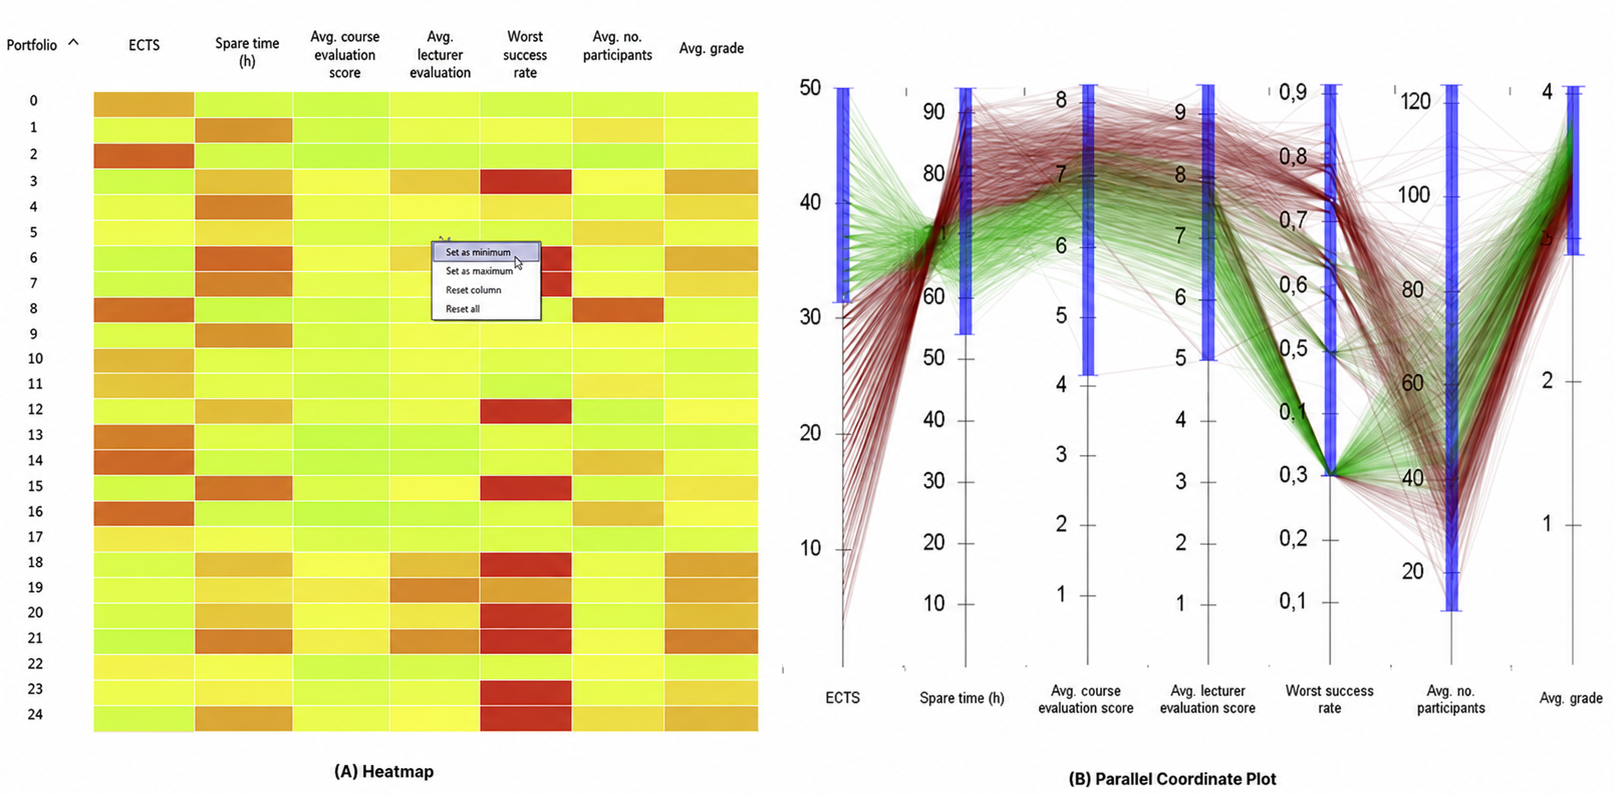
\includegraphics[width=6in]{Figures/HeatmapAndPCP.png} % ≤ 6 inches wide
    \caption[An example of a tabular heatmap and a PCP application for visualizing the alternatives' performance]{The application of a tabular heatmap (A) and a parallel coordinate plot (PCP) chart (B) to visualize the performance of several alternative solutions across multiple criteria (adopted directly from Gettinger et al.~\cite{gettinger_comparison_2013}).}
    \label{heatmapAndPCP}
\end{figure}
The results of the user study conducted by Gettinger et al.~\cite{gettinger_comparison_2013} show that PCP users perform the entire decision process faster than users of (textual) tables and heatmaps for tasks with a smaller number of criteria and alternatives. As the number of criteria and alternatives increases, this particular advantage of PCP starts to disappear due to an increase in the number of visual marks and channels, causing visual cluttering (specifically when there are more conflicting decision options in the decision space). However, PCP users take more steps and iterate more frequently back and forth to reach a final set of admissible solutions, while heatmap and table users performed fewer filtering steps than PCP users and showed less dynamic exploration. From all of these results, we can eventually conclude that \textbf{decision tables and heatmaps are functionally more appropriate for programmed and semi-programmed decision problems} (in which the decision-making process is more structured and straightforward), while \textbf{PCPs align better with non-programmed decisions} as they support exploration and the agility needed for the ill-structured nature of non-programmed decisions.\par
In addition to PCPs and tabular heatmaps, other visualization techniques and chart types can also be utilized in the choice stage for evaluation and comparison of discrete alternatives based on multiple decision criteria. In Figure ~\ref{stackedBar}, for example, a vertically stacked bar graph from Angelis et al.~\cite{angelis_early_2020} has been used to demonstrate the aggregate scores of four different medical treatment compounds (labeled with A, B, C, and D) as alternatives in several health-tracking criteria (labeled with capital letters like DELI) in a single bar graph. The normalized value of every alternative compound in each criterion in this case has been encoded by the length of a bar of a color unique to every criterion. As the criteria might be of different measuring units, their corresponding values have been normalized so that they can all be visualized alongside a common length channel.\par
\begin{figure}
    \centering
    % Ensure figure width fits within SFU margins
    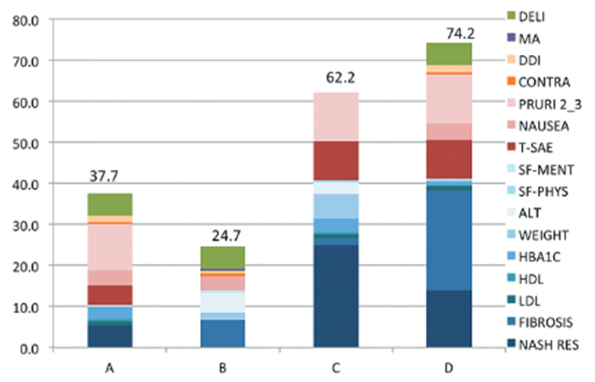
\includegraphics[width=6in]{Figures/StackedBarGraph.png} % ≤ 6 inches wide
    \caption[A stacked bar chart for visualization of alternatives' performance]{A stacked bar graph visualizing the normalized and aggregate performance values of four different medical treatment alternatives (A, B, C, and D) across several healthcare criteria (adopted directly from Angelis et al.~\cite{angelis_early_2020}).}
    \label{stackedBar}
\end{figure}
As a data-level task, designing visualizations for \textit{value comparison} is informed by many rules and best practices that DSS designers should consider. For example, according to Cleveland and Mcgill~\cite{cleveland_graphical_1984}, quantitative comparisons should be made using position along a common scale whenever possible, rather than comparing lengths, areas, angles, or positions on separate scales. Since bar charts encode values as lengths measured from a common baseline, the authors recommend arranging bars so that their endpoints can be compared against the same aligned axis. Applying this rule to the context of comparing multiple alternatives' performance in separate criteria, a grouped bar chart instead of a stacked bar chart should be used to visualize the criteria values separately if no preference weight or objective function is known to aggregate the values of an alternative in all criteria into a single final score.\par
In addition to the situations in which the decision space is finite, there are cases in which the decision levers are inherently continuous variables that can obtain infinite (or even too many) values between any two values in their range. Several approaches can be taken to visualize the outcomes of decisions with continuous levers based on the number of levers and outcomes. The simplest form of problem that has one single lever and one outcome can be simply visualized by a 2D graph in which one axis (usually the horizontal) is reserved to encode the possible values of the lever, and the other axis encodes the resulting value of the outcome. Having two levers (of which at least one is continuous) and a single outcome can also be visualized either by a 2D contour plot/heatmap or by a 3D surface plot. In Figure ~\ref{contours}, we can see an example of both of these visualizations for finding the maximum value of specific surface area (as the outcome) of a chemical compound as a function of hydrothermal temperature (1\textsuperscript{st} lever) and reaction time (2\textsuperscript{nd} lever), adopted from Raduwan et al.~\cite{raduwan_application_2024}.\par
\begin{figure}
    \centering
    % Ensure figure width fits within SFU margins
    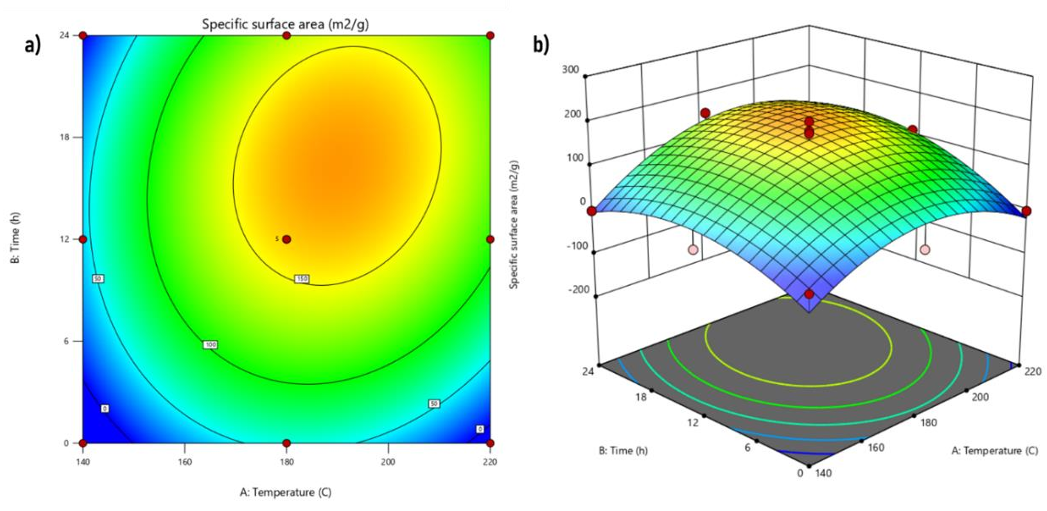
\includegraphics[width=6in]{Figures/ContourMaps.png} % ≤ 6 inches wide
    \caption[Application of contour maps for visualizing the value of a single objective function across different combinations of values of two independent variables]{Application of (A) 2D and (B) 3D contour maps visualizing the value of specific surface area variable across different ranges of values for two continuous variables (i.e., \textit{Time} and \textit{Temperature}). Color and Hue visual channels have been employed to differentiate between different ranges of values for surface area (dark-yellow for the highest value to dark-blue for the lowest values). Convexness of the response surface in (b) has made the usage of contour lines possible (adopted directly from Raduwan et al.~\cite{raduwan_application_2024}).}
    \label{contours}
\end{figure}
In Figure ~\ref{contours} (A), each level of values of specific surface area has been distinguished with an oval shape contour line and color-coded with a distinct color and saturation. In Figure ~\ref{contours} (B), the complete range of specific surface area values is shown on the z-axis. Despite being less cognitively demanding than 2D graphs, a 3D surface plot like the one in Figure ~\ref{contours} (B) can be particularly helpful when any small change in the levers’ values would result in a drastic non-linear change in the value of the outcome response. In such cases, 2D contour lines and color-coded maps would become too cluttered and less sensible to users due to the heterogeneity of the contour areas ~\cite{munzner_visualization_2015}.\par
Another case is the existence of multiple outcomes with similar dimensions and a single continuous lever variable. Having similar measurement units, the values of different outcomes can be superimposed into a single graph in which an axis encodes the continuous values of the lever, while the other axis encodes the values of outcomes altogether. However, if the measuring units of the outcomes are not all alike, the distribution of the outcome values over those of the levers can be visualized by separate juxtaposed graphs.\par
\begin{figure}
    \centering
    % Ensure figure width fits within SFU margins
    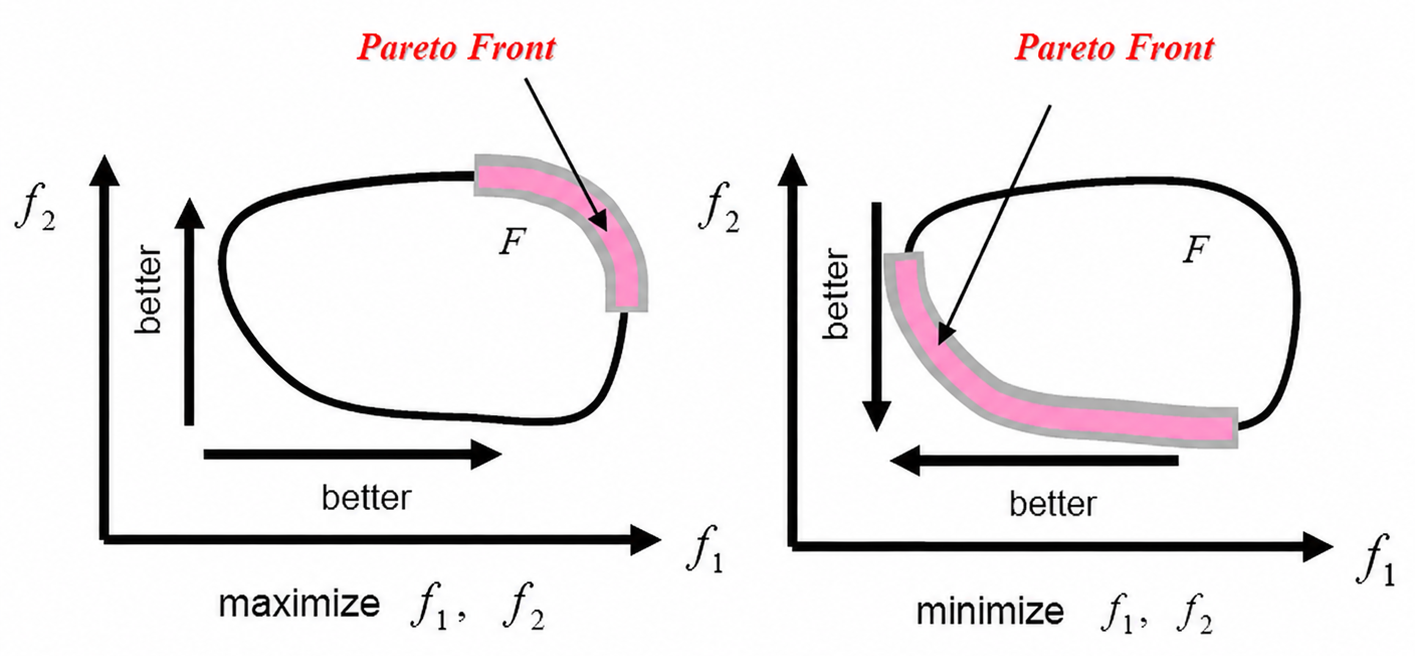
\includegraphics[width=6in]{Figures/Biobjective_VIZ.png} % ≤ 6 inches wide
    \caption[Application of 2D maps for visualizing all possible values for the objective functions of bi-objective decision problem]{2D maps visualizing the boundaries of possible values of two hypothetical objective functions (i.e., $f_1$ and $f_2$) across a continuous solution space. Assuming that (Left) an increase, or (Right) a decrease in the value of both functions is desired, the optimal solution to the decision problem lies on the \textit{Pareto front} curves (adopted directly from Ngatchou et al.~\cite{ngatchou_pareto_2005}).}
    \label{biobjective_viz}
\end{figure}
When the number of levers becomes more than one, while we have two outcomes (a bi-objective decision problem), a 2D graph can be constructed to visualize all the possible values of both outcomes upon a specific set of values of all the levers. In Figure ~\ref{biobjective_viz}, we can see an example from Ngatchou et al.~\cite{ngatchou_pareto_2005} in which all the possible values of two outcomes $f_1$ and $f_2$ have been shown on two 2D graphs. In Figure ~\ref{biobjective_viz} (left), the larger values for both $f_1$ and $f_2$ are desired; therefore, the values of these two outcomes that land on the left side of the decision space perimeter are certainly not the optimal outcomes, as there are points over the perimeter of the same space that deliver a more desired value for both outcomes. In Figure ~\ref{biobjective_viz} (right), the smaller values for both $f_1$ and $f_2$ are desired, making the bottom-left corner of the decision space's perimeter possess non-dominated solutions to this hypothetical bi-objective optimization problem. In both cases, the point of optimal values of the outcomes is a point from the outermost surface of the space’s perimeter (stroked and highlighted with pink) called \textit{Pareto front}, in which \textbf{no point delivers a better value for an outcome without worsening the other}. In this case, the decision-maker should evaluate and consider taking the actions that result in the outcomes landing on the Pareto front curve.\par
Finally, the number of continuous levers and heterogeneous outcomes may go beyond a few. In such scenarios, the above-explored visualization structures fall unable or unhelpful to represent all the outcomes’ values of a continuous decision space in a 2D or a 3D graph at once; therefore, an interaction between the user who specifies the lever variables’ values for which he wants to view the outcomes for and the system which simulates and renders the outcomes for the values that user had set for levers becomes inevitable. This interaction can, of course, happen both synchronously and asynchronously; yet, many researchers have advocated for a synchronous interaction between the user and the visualization interface in decision support systems ~\cite{pugmire_visualization_2016,heer_interactive_2012,ashok_visualization_2008,jain_effectiveness_2006}. As discussed before, the application of interactive visual idioms is crucial for realizing a real-time visualization of the requested portion of the whole dataset. These idioms enable users to adjust values of the parameters and the variables (i.e., decision levers in this particular context) to their liking, and the system will fetch/generate the output data (i.e., decision outcomes in this context) and render it back on the user interface in the form of a visualization. In Figure ~\ref{interactiveOutcome}, an example of an interactive decision support system interface—visualizing the outcomes of Switzerland’s electricity supply sources policies—has been adopted from Xexakis and Trutnevyte~\cite{xexakis2019interactive} and shown. In this example, the user can specify the exact value of each continuous decision lever—that is, the percentage (\%) of an electricity supply source usage from the total source’s potential—by adjusting its corresponding slider’s place in its permissible range of values. The system, in response, handles the event of the slider’s movement synchronously and updates the values of the electricity supply (top-middle panel), the proportion of the electricity supply sources in the mixture (top-right panel), and the undesired impact level caused to each environmental criterion (bottom panel).\par
\begin{figure}
    \centering
    % Ensure figure width fits within SFU margins
    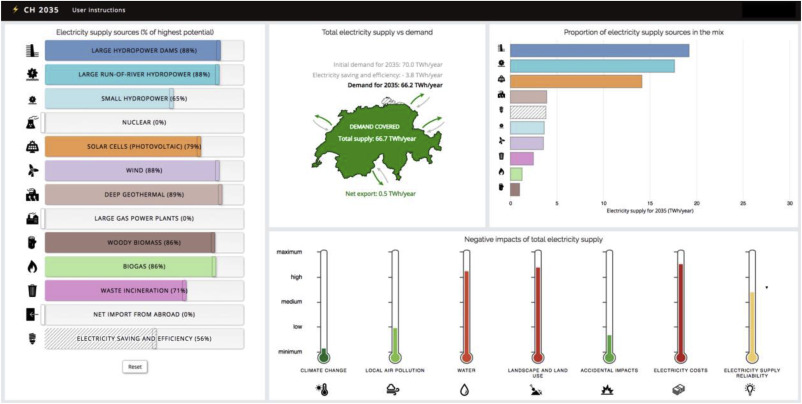
\includegraphics[width=6in]{Figures/InteractiveOutcomeVIZ.jpg} % ≤ 6 inches wide
    \caption[An example of an interactive dashboard for the real-time visualization of policy outcomes]{An interactive dashboard to synchronously evaluate and compare the economic and environmental outcomes of different electricity supply chain policies encoded by the different sets of values for decision levers, encoded by a group of sliders in the left panel. Upon every movement of any slider in its permissible range, the policy outcomes are updated in real-time in the top-right and bottom panels (adopted directly from Xexakis and Trutnevyte~\cite{xexakis2019interactive}).}
    \label{interactiveOutcome}
\end{figure}
his interactive approach for visualizing the outcomes for a specific set of inputs can also be utilized to represent the outcomes of a particular choice when the number of all alternatives is finite, despite the existence of several visualization structures for representing all the outcomes of the decision problems with a finite set of alternatives all at once. This, for instance, has been realized in a DSS proposed by Accorsi et al.~\cite{accorsi2014decision} for a warehousing system in which the values of cost-and-benefit \textit{key performance indicators (KPIs)} as the outcomes are generated and shown in real-time when the user selects a specific value out of four possible options for allocation strategy as the lever variable.\par
Even when the decision space is continuous or contains too many solutions, DMs might only be interested in investigating the outcomes of a few specific decision scenarios out of all the possible scenarios. A common way to address this need is to juxtapose the static visualizations of the values for the decision levers and the outcomes in every scenario of interest. In this way, users can easily compare the outcomes of different decision scenarios caused by differences in the input values for levers or exogenous variables. Back to the example from Xexakis and Trutnevyte~\cite{xexakis2019interactive}, four different decision scenarios for Switzerland’s electricity supply resource management have been visualized in a 2×2 juxtaposition as shown in Figure ~\ref{scenarioVIZ}.\par
\begin{figure}
    \centering
    % Ensure figure width fits within SFU margins
    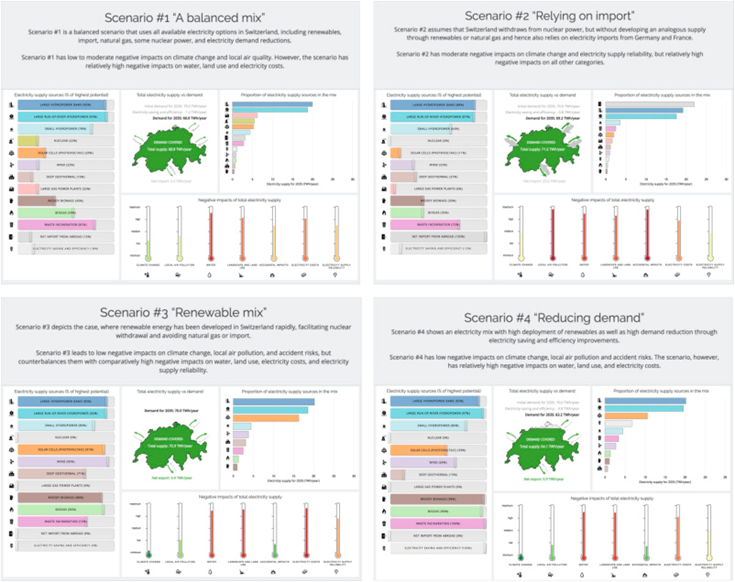
\includegraphics[width=6in]{Figures/scenarioVIZ.png} % ≤ 6 inches wide
    \caption[Juxtaposition of different decision-making scenarios for facilitated comparison]{Juxtaposition of four static views—corresponding to four electricity supply chain policy scenarios—to facilitate comparison of different policies’ outcomes (adopted directly from Xexakis and Trutnevyte~\cite{xexakis2019interactive}).}
    \label{scenarioVIZ}
\end{figure}
As seen in Figure ~\ref{scenarioVIZ}, different decision scenarios are related to the different values for the percentage (\%) of every electricity supply source usage from the total source’s potential as the levers that have resulted in different levels of negative impact on environmental factors as the outcomes. The results show that the electricity demand reduction policy (scenario\#4) would provide the least amount of negative impact on all environmental factors, compared to the first three scenarios. However, scenario\#4 is heavily relying on electricity demand reduction, which is an exogenous factor and not in the hands of the decision-making team. On the other hand, the occurrence of the first three scenarios is dependent on DMs’ intent and actions, and the outcomes of these show mixed impact levels on different categories of environmental factors.
\subsubsection{Algorithmic Decision-making: The role of AI Agents and Mathematical Optimization (MO)}
One of the very last steps in the whole process of decision-making, according to Simon’s three-stage model, is selecting the alternative (for discrete decision spaces) or developing the set of actions (for continuous decision spaces) that provide the most desirable performance across different criteria or outcomes. Despite more DM-centered approaches in which DM manually compares the solutions’ outcomes’ desirability with the aid of simulation and visualization techniques discussed earlier to find the optimal solution, there are also fully automated and semi-automated approaches for organizational decision-making to solve a preformulated and programmed decision problem. We refer to fully automated decision-making as the decision-making process in which computational methods (e.g., AI algorithms) discover and deploy the optimal solution to a well-defined decision problem without human intervention, while semi-automated decision-making is a process that involves both human DMs and computational agents in the decision-making loop. The latter process itself can also be realized in a sequential form or aggregated (parallel). In the sequential form of semi-automated decision-making, the human DM and computational agent provide an output which becomes the input for the other, and can be either of the following modes:\par
\textbf{I. Human decisions as input to algorithmic decision-making:} Human DM narrows down the whole solution set into a set of refined solutions and provides the latter set to the computational agent for further evaluation and selection of the optimal solution.\par
\textbf{II.	Algorithmic decisions as input to human decision-making:} Unlike the previous mode, the computational agent this time goes through the whole solution set and narrows it down into a set of refined solutions and passes the latter set to human DM for selection of the optimal solution.\par
The aggregated form of semi-automated decision-making, on the other hand, involves both computational agent and human DMs as independent decision-makers on the same problem, for which they each come up with their own solution, before an aggregated solution is derived by means like polling or weighted averages. The strengths and weaknesses of every above-mentioned model have been summarized by Shrestha et al.~\cite{shrestha_organizational_2019} against five different conditions in Table ~\ref{AIforDecision}.\par
\begin{landscape}
\begin{table}
\centering
\small
\caption{General comparison of different models of human-AI involvement in organizational decision-making (adopted from Shrestha et al.~\cite{shrestha_organizational_2019}).}
\label{AIforDecision}
\begin{tabular}{p{5cm} p{4cm} p{4cm} p{3cm} p{3cm} p{2cm}}
\hline
Model & Specificity of the Decision Search Space & Interpretability & Size of the Alternative Set & Decision-Making Speed & Replicability \\
\hline
Fully-automated  & High   & Low  & Large & Fast  & High  \\
Manual & Low & High & Small & Slow & Low  \\
Sequential Semi-automated I: Human to AI  & Low → High & Low & Small & Slow & Low \\
Sequential Semi-automated II: AI to Human & High → Low & High & Large & Slow & Low \\
Aggregated Semi-automated & Low (for human decision) & High (for human decision) & Small & Slow & Partial \\
\hline
\end{tabular}
\end{table}
\clearpage
\end{landscape}
According to Shrestha et al.~\cite{shrestha_organizational_2019}, deployment of computational agents such as AI algorithms to fully-automate the decision-making process without human intervention is particularly more appropriate when (i) the speed and replicability of the process have to be high, (ii) the number of alternatives is too many, (iii) the decision space is highly-specified, and (iv) interpretability of the decision-making process is less important. In addition to these conditions, fully-automated decision-making can only take place in circumstances when there is only one objective function (final criterion) to evaluate the alternatives according to. The examples for this model pertain to online product recommendation systems, dynamic pricing systems, and fraud detection systems ~\cite{shrestha_organizational_2019}. The deployment of algorithmic decision-making, however, is not without societal and humanistic challenges at all. Science, technology, and society (STS) studies have pointed out the biases that such algorithms may inherit from their designers and creators, questioning the objectivity and rationality of their final choices ~\cite{barocas2016big}.\par
On the other hand, manual decision-making might become inevitable or even preferred when (i) the decision space and outcomes are not computationally specified, but loosely defined, (ii) interpretability and transparency of the decision-making process is of a high importance, (iii) the number of alternatives is not too many to handle, and (iv) the speed and replicability of the process are not critical factors to DM ~\cite{shrestha_organizational_2019}.\par
In sequential semi-automated scenarios, when a computational agent provides a refined set of solutions to DMs, the interpretability of the made decisions is still high because of human involvement in making the final decision. As it is the computational agent that goes through the initial set of solutions to select a few better options for later human decision-making, the size of the initial alternatives set can be large, yet the decision space has to be computationally specified. Human involvement makes this process low in replicability and slow-paced. Loan application systems, crowd-sourcing platforms, and hiring systems are among the examples of algorithm-first sequential semi-automated decision-making ~\cite{shrestha_organizational_2019}.\par
The other sequential semi-automated decision-making process is led by human decision-makers who refine the initial set of alternatives into a few considered solutions, which are computationally specified before being given to the computational agent for choosing the most suitable one. In this process, the interpretability of the made decisions is low, as the final decision is made by the computational agent. Moreover, the replicability and the decision-making speed in this process both fall victim to human involvement. The initial set of alternatives cannot also contain too many solutions, as it may become ever-tedious for human DMs to investigate them all. Shrestha et al.~\cite{shrestha_organizational_2019} reported the deployment of this type of sequential semi-automated decision-making process in some sports analytics and health monitoring systems.\par
Finally, the aggregated semi-automated decision-making process treats the computational agent as an independent decision-maker whose choices can, to some extent, contribute to the final decision made alongside those of human DMs. This would make the interpretability and replicability of the made decisions low and high for algorithmic decisions, and high and low for human decisions, respectively. Since the same alternatives set is given to both human DM and computational agent, the size of the alternatives set is still limited by human DM’s cognitive capacity and cannot be too large. The speed of the overall process is slow and bottlenecked by human DMs. For algorithmic decisions, the decision search space as well as the objective function both need to be specified so that the decision-making algorithm can operate well. Top organizational management teams and boards can utilize this aggregated semi-automated decision-making model for making strategic or executive decisions ~\cite{shrestha_organizational_2019}.\par
In the context of our framework, the application of each of the above processes is dependent on the structure and nature of the decision problem as well as those conditions highlighted in the research from Shrestha et al.~\cite{shrestha_organizational_2019}. If a causal decision model involves quantified outcomes in a way that the different solutions can be numerically evaluated and compared, a computational decision assistant can be developed to rank different solutions’ performance in every criterion (outcome) and rule out those that underperform in all aspects. Such a computational assistant can utilize different algorithms to discover the optimal solution/alternative depending on the data types of the levers. Multi-objective optimization (MOO) is a family of algorithms utilizing the concept of Pareto optimality to search the decision space and discover a set of non-dominated solutions as candidates for the final choice. Among all MOO algorithms, those that work when the objective functions are unknown are best-fitted within our framework. The reason for that is that the outcome variables in our assumed causal decision model are measured by a chain of structural equations that are susceptible to becoming too complex as the developed causal network grows. Labeled as \textbf{black-box optimization (BBO)} algorithms, many researchers have proposed different classes of BBO algorithms under different assumptions. According to Bajaj et al.~\cite{bajaj2021black}, when there is no constraint applied to decision levers’ values, the following classes of BBO algorithms may be employed to extract a set of Pareto optimal solutions:\par
\textbf{I. Direct Search Methods:} Includes methods such as \textit{Simplex Search, Coordinate Search, Nelder-Mead, Generalized Pattern Search (GPS),} and \textit{Mesh Adaptive Direct Search (MADS)}.\par
\textbf{II. Model-based Methods:} Includes \textit{Model-based Trust Region} and \textit{Project-based} Methods.\par
\textbf{III. Heuristic Methods:} Includes \textit{Simulation Annealing (SA), Genetic Algorithm (GA), Particle Swarm Optimization (PSO), Branch and Bound, Surrogate Management Framework (SMF), Hit-and-Run Algorithms, Multilevel Coordinate Search (MCS),} and \textit{DIRECT}.\par
\textbf{IV.	Hybrid Methods:} Combines a set of algorithms from the above-listed classes, such as \textit{PGS-COM}, combining PSO and COMPLEX algorithms for solving constrained non-smooth black-box optimization problems, introduced first in a research by Martelli and Amaldi~\cite{martelli2014pgs}.\par 
On the other hand, when constraints have been applied to the values that decision (lever) variables can possess, other classes of algorithms, such as \textit{Penalty Method, Augmented Lagrangian, Filter Method,} and \textit{Surrogate Modeling}, can be employed ~\cite{bajaj2021black}. In order to implement these algorithms in a computational decision assistant, computer solvers have already been developed to be imported for solving BBO problems, both in the form of software packages such as TOMLAB (MATLAB optimization environment) and open-source programs such as Pymoo (a Python library for multi-objective optimization).\par  
Once a set of Pareto-optimal solutions is generated by the computational decision assistant, it can either be passed to the human DM for the manual selection of the final choice or be given as the input to another computational decision agent to introduce the globally optimal choice if the human DM’s preferences are clear and already declared ~\cite{osika2023multi}. Earlier, we showed how visualization structures such as PCPs and multidimensional graphs with contour lines can aid DMs in comparing solutions in discrete and continuous decision search spaces. However, when DM’s preferences are given as a set of numerical weights, computational systems can rely on several mathematical methods called \textbf{multi-criteria decision-making (MCDM)} to select an optimal final choice automatically.\par
Decision problems with a discrete set of candidate solutions can primarily be solved by the multi-attribute decision-making (MADM) family of methods, while the problems with a continuous set of candidate solutions require the \textbf{multi-objective decision-making (MODM)} category of methods to be solved. In Figure ~\ref{MCDMTree}, a classification tree of different MCDM methods has been adopted from Gebre et al.~\cite{gebre2021multi} and demonstrated.\par
\begin{figure}
    \centering
    % Ensure figure width fits within SFU margins
    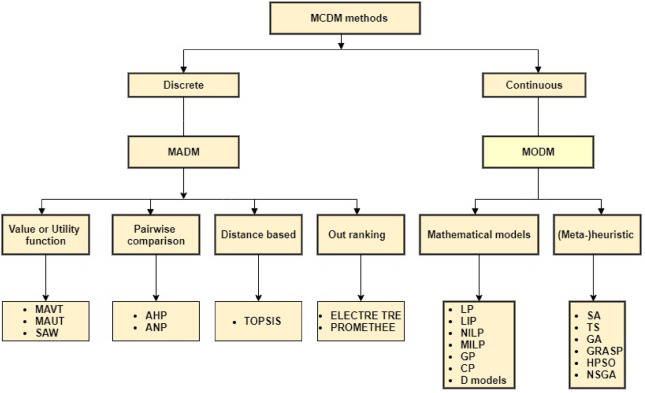
\includegraphics[width=6in]{Figures/MCDMTree.jpg} % ≤ 6 inches wide
    \caption[Classification of MCDM methods]{Different classes of multi-criteria decision-making (MCDM) methods. Methods that solve problems with a discrete/finite set of alternatives are categorized as multi-attribute decision-making (MADM) methods, while those dealing with a continuous/infinite set of solutions are classified as multi-objective decision-making (MODM) problems (adopted directly from Gebre et al.~\cite{gebre2021multi}).}
    \label{MCDMTree}
\end{figure}
As seen in Figure ~\ref{MCDMTree}, MADM methods, which solve problems with a discrete set of alternatives, are themselves classified into value/utility function methods, pairwise comparison methods, distance-based methods, and outranking methods, described in detail as follows:\par
\textbf{I. Value or Utility Function Methods:} Use utility theory (UT) to rank alternatives based on multiple (and often conflicting) criteria. Includes \textit{multi-attribute value theory (MAVT), multi-attribute utility theory (MAUT)}, and \textit{simple additive weighting (SAW)} algorithms.\par
\textbf{II. Pairwise Comparison Methods:} Use two-by-two comparisons of all criteria/sub-criteria importance according to DM’s judgement. Includes \textit{analytical hierarchy process (AHP)} and \textit{analytical network process (ANP)} algorithms. \par
\textbf{III. Distance-based Methods:} Measure and compare alternatives’ distance from an ideal or negative-ideal solution. Depending on the type of measured distance (e.g., Euclidean, Manhattan), includes Technique for Order of \textit{Preference by Similarity to Ideal Solution (TOPSIS), Combinative Distance-based Assessment (CODAS), Combined Compromise Solution (COCOSO), Characteristic Objects Method (COMET),} and \textit{Weighted Euclidean Distance-Based Approach (WEDBA)}.\par
\textbf{IV. Outranking Methods:} Are used to rank, select, or sort a set of alternatives by performing pairwise comparisons across various, often conflicting, criteria. Includes \textit{Elimination and Choice Expressing Reality (ELECTRE)} and \textit{Preference Ranking Organization Method for Enrichment of Evaluations (PROMETHEE)}.\par
In addition, fuzzy variants for many of the above techniques have been introduced in the literature when the alternatives’ performance in every criterion is a fuzzy set rather than a single pre-determined value ~\cite{aouam2003fuzzy}. The examples include fuzzy-TOPSIS ~\cite{nadaban_fuzzy_2016} and fuzzy-AHP ~\cite{chang1996applications}.\par
MODM methods—which come up with a final choice from a continuous set of candidate solutions—depend on the following precise mathematical models or metaheuristic algorithms to reach a final choice among an infinite number of candidate solutions:\par
\textbf{I. Mathematical Models:} Are algorithms that find the optimal solution accurately from an infinite set of candidate solutions (Pareto optimals). Includes \textit{Linear Programming (LP), Linear Integer Programming (LIP), Non-linear Integer Programming (NLIP), Mixed-integer Linear Programming (MILP), Goal Programming (GP), Compromise Programming (CP),} and \textit{Dynamic (D) Models}.\par
\textbf{II. Metaheuristic Algorithms:} Leverage some of the previously explained MOO algorithms (in single-objective format if DM’s preferences are directly given) to “guess” the optimal final choice, which might not necessarily be the same as the best possible choice. Includes \textit{Simulation Annealing (SA), Tabu Search (TS), Genetic Algorithm (GA), Greedy Randomized Adaptive Search Procedure (GRASP), Hybrid Particle Swarm Optimization (HPSO)}, and \textit{Non-dominated Sorted Genetic Algorithms (NSGA)}.\par
The decision of which specific method should be used to solve an MCDM problem has also been addressed in the literature to some extent, depending on a few factors. Cinelli et al.~\cite{cinelli2022recommending} found a list of both abstract and granular information elements affecting the choice of the most suitable method to solve an MADM problem through an extensive literature review and developed a decision support system (DSS)—called “MCDA-MSS”—to recommend the most suitable method(s) according to each MADM problem case study's characteristics. All these important factors for selecting the most suitable MADM method are gathered by answering questions regarding:\par
\textbf{I. Decision problem’s typology} like “\textit{Is the structure of the criteria flat or hierarchical?}”,\par
\textbf{II. Preference model} like “\textit{How should the comparison of the performances on the criteria be performed?}”,\par
\textbf{III. Elicitation of preferences} like “\textit{Should precise or imprecise weights be used in this case study?}”, and \par
\textbf{IV. Exploitation of the preference model} like “\textit{How should the output variability analysis be conducted?}”.\par
Once the answers to these questions (which all invoke either binary or multiple-choice responses) are collected and processed into the DSS, the system searches among its MADM methods’ database to fetch the method(s) with the greatest number of matching characteristics with those of the answers and returns them to the UI as method recommendations ~\cite{cinelli2022recommending}. For example, when DM chooses to have a complete ranking of all alternatives, methods such as AHP or PROMETHEE II are recommended by the DSS to fulfill that particular need. The selection of a suitable MADM method can particularly be crucial as different methods may (and often do) give different optimal alternatives even if the provided preference vector stays the same ~\cite{karami2014short,mulliner2016comparative}. However, without method selection, the scores or rankings of alternatives brought by different methods can all be visualized for DMs, enabling them to recognize possible convergence of different methods to a particular alternative as the optimal choice.\par
Similar to MADM, MODM methods (even the accurate ones) do not necessarily converge to a single optimal solution or a set of Pareto optimal solutions because of the differences in the ways they treat the problem’s information, including preferences. As explained earlier, among the whole family of MOO and MODM algorithms, the algorithms that do not rely on the objective functions’ gradient (gradient-free algorithms) are assumed to be only pragmatically consistent with our simulation-driven framework. Among gradient-free methods, \textbf{multi-objective evolutionary algorithms (MOEAs)}—a subset of heuristic multi-objective algorithms—such as the NGSA class of algorithms (e.g., NGSA-II) are prominent due to their flexibility, globality, and relative ease of use ~\cite{deb2011multi}. However, because of their dependence on population sampling, MOEAs are of a stochastic nature and result in a different optimal solution in every run. In addition, MOEAs are computationally intensive, and it can take a long time for them to converge to a non-dominated solution. On the contrary, Direct Search methods (e.g., Nelder-Mead, GPS, and MADS) are more time-efficient, deterministic, and converge to non-dominated solutions more quickly. Unlike MOEAs, which are sampling-based, Direct Search methods rely on local refinement, making them susceptible to being trapped by local and not global optimal solutions. Therefore, they should be carefully used when the decision problem is complex and has a non-convex shape for the solution set ~\cite{cano2022out}. When the efficiency is a critical factor, and at the same time, either a global set of Pareto optimal solutions is required, or the problem is too complex to use direct search methods, the following approaches are recommended:\par
\textbf{I. Enhance MOEAs’ efficiency by integrating them with surrogate models}, which is best realized in \textbf{surrogate-assisted evolutionary algorithms (SAEAs)} such as ParEGO, balancing computational cost with solution accuracy. SAEAs work best when the objective function evaluations are time-consuming and highly expensive ~\cite{kudela_comparing_2024}.\par
II. \textbf{Use non-evolutionary (meta-)heuristic multi-optimization algorithms}, such as PSO/SA, to efficiently discover global “good-enough” solutions with low computational costs. Work best when the objective function evaluations are inexpensive and take only a few seconds. \par
III. \textbf{Use decomposition-based MOEAs, such as MOEA/D}, that break multi-objective problems into smaller scalar optimization subproblems, solving them simultaneously using neighborhood information, offering faster convergence and better distribution, especially when there are many (typically more than 3) objective functions ~\cite{zhou_decomposition-based_2021}.\par
Evolutionary algorithms converge to a more accurate set of candidate solutions than non-evolutionary algorithms in many MOO problems eventually. However, when higher levels of accuracy are required, hybrid MOEAs that integrate the exploration capabilities of standard MOEAs with the exploitation capabilities of local search operators can be employed. An example of such a hybrid MOEA has been proposed in a research by Debrel~\cite{derbel2025simple}, which enhances the accuracy of standard MOEAD with local search operators.\par
Each of the above MOO approaches can also be employed for the selection of the final optimal choice in the context of the MODM problem when DM’s preferences are priorly given. Using DM’s numerical preferences as objective functions’ weights, all the objective functions can be aggregated into a single objective function. This process is called \textbf{\textit{scalarization}}, and can happen in either one of the following forms:\par
\textbf{I. Weighted Sum Scalarization (WSC):} uses a linear utility function to construct the aggregate objective function.\par
\textbf{II. Weighted Tchebycheff Scalarization:} uses a curvature L-distance utility function to construct an aggregate objective function that measures the maximum weighted distance of all objective functions from their ideal value.\par
\textbf{III. $\epsilon$-Constraint Method:} tries to find solution(s) that optimize one of the objective functions while treating other objective functions as constraints that are bounded to $\epsilon$ values.\par
\textbf{IV. Weighted Goal Programming (WGP):} considers the aggregate objective function as the weighted sum of deviations from target values (goals) for every objective function.\par
DM’s preferences can also be given as input to some MOO algorithms iteratively in the course of optimization ~\cite{osika2023multi}. Certain interactive MOO algorithms (e.g., IEMO/D) allow DMs to guide the solution search process toward the areas of the Pareto front that are more preferred, by prompting them to provide their preferences iteratively via either one of the following ways ~\cite{thiele2009preference}:\par
\textbf{I. Target values (i.e., aspiration levels) for each objective function:} that act as a reference point on the Pareto front. It is supported by algorithms such as the \textit{non-differentiable interactive multi-objective bundle-based optimization system (NIMBUS)}, reference point NSGA-II (R-NSGA-II), and \textit{interactive generalized differential evolution 3 (I-GDE3)}. \par
\textbf{II. Indirect preferences (e.g., ranking/evaluation) of two or multiple solutions:} to make the search algorithm learn DM’s preference over several algorithms’ runs. It is supported by algorithms such as the \textit{dominance-based rough set approach (DRSA)}, progressively interactive NSGA-II (PI-NSGA-II), and \textit{interactive decomposition-based evolutionary multi-objective optimization (IEMO/D)}.\par
From the above two ways via which the DM’s preferences are articulated interactively over the course of optimization, reference-based methods converge faster toward the desired solutions near the Pareto front early on, if the aspiration levels for all objectives are accurately expressed. On the other hand, interactive algorithms requiring the declaration of indirect preferences may take a higher number of iterations and DM’s feedback to converge toward a desired set of solutions near the Pareto front. The efficiency in this type of algorithm, however, is sacrificed for enhanced explainability and lower levels of cognitive load for DMs ~\cite{taylor2021bayesian}. In a nutshell, the former aspiration-based interactive MOO algorithms are better suited for when optimization process’ efficiency is critical and/or DM possesses a high degree of knowledge about objective functions’ goals, while the latter class of interactive MOO algorithms are better aligned with circumstances in which DM has a lower level of knowledge and expertise about the problem’s goals; thus, needs careful evaluation of recommended solutions after every iteration ~\cite{taylor2021bayesian}. The process of eliciting DM’s preferences in latter interactive MOO algorithms can also be augmented by interactive visualization of the outcomes of two or multiple solutions, prompting the user to select the desired solution or assign preference ranking to the visualized solutions set for progressing towards an ultimate set of desired solutions ~\cite{thiele2009preference}.
\subsubsection{Sensitivity Analysis and Assessing Solutions' Robustness}
The desired impact of a developed solution for tackling a decision problem is always subject to environmental noise and unforeseen consequences. An ill-defined causal structure, inaccurate measurement of causal interactions between decision variables, and false evaluation of external parameters are the reasons why an adopted solution does not lead to the most desired outcomes for DMs in a decision-making problem. \textbf{Sensitivity analysis (SA)} is an activity in which the reliability of the solutions that DMs develop to solve a decision problem is assessed against the possible changes in the presumed values of the model’s exogenous factors ~\cite{rappaport1967sensitivity,hekimouglu2010sensitivity}. An alternative or solution to a decision problem can be the most preferred choice under some conditions or certain values of the exogenous variables, but it would become less desirable or lose its advantage over other solutions if the exogenous variables’ values change. Therefore, DMs should check the responsiveness of the outcomes of every solution they have developed over different values for external variables and parameters before choosing one to implement.\par
Formal approaches to sensitivity analysis have been developed over the years by researchers from different disciplines. In the field of \textbf{Operations Research (OR)}, for example, Rappaport~\cite{rappaport1967sensitivity} introduced a decision-tree-based approach for analyzing the expected value of outcomes of every alternative as the basis of discrete alternatives ranking when the outcomes for every alternative are not deterministic and subject to change. Despite framing SA and its variations in a classic linear programming problem, no formal method is provided by Rappaport~\cite{rappaport1967sensitivity} for taking the probability distribution of different extents of change in exogenous factors into account when the decision space is infinite. This is particularly important as a variation in one of the environmental decision factors during implementation may be unlikely but of great consequence, and vice versa. Therefore, DMs need to consider both the significance and the probability of occurrence of an alteration on pre-assumed values of the external factors when investigating different solutions to the decision problem. Saltelli et al.~\cite{saltelli2000sensitivity} have provided a stochastic and mathematical formalization for the SA process under different methods and assumptions. One common assumption is that the variation in the model’s output is studied when only \textbf{one factor changes at a time (OAT)}, while the values of other factors are held constant. They have also formalized SA for both when the changes happen around a single local point of input values and when the changes take place over the whole range of inputs’ permissible values. The former method—\textbf{local sensitivity analysis (LSA)}—is more beneficial for circumstances in which the variations in input parameters are expected to take place around a central point of data, while the latter—\textbf{global sensitivity analysis (GSA)}—is more appropriate for the cases in which the actual values of input parameters may be at any random distance from the assumed value ~\cite{saltelli2000sensitivity,saltelli2008global}.\par
The main purposes of performing SA in studies such as those from Saltelli et al.~\cite{saltelli2000sensitivity,saltelli2008global} are to discover the factors that cause the most and least volatility in the computational model’s output, as well as the calibration and adjustment of the model’s parameters and variables. In addition to not being perfectly aligned with our decision-oriented perspective—for which we are interested to see whether variation in both lever and exogenous variables’ values results into outcomes that would have been better if another solution was adopted under the new condition—, the extensive computational jargon of these works makes their formal approach to SA too difficult for DMs and users of other disciplines to embed in their decision-making systems and processes. Therefore, a more practical and agile approach shall be adopted as the baseline activity to analyze the sensitivity of solutions to a decision problem, answering “\textit{Does parameter variation invalidate the original decision?}” instead of traditional SA, which answers “\textit{Is the model output sensitive to parameter changes?}”, shifting the focus from model robustness to decision robustness. We now formalize a decision-oriented sensitivity analysis framework, going beyond traditional parameter perturbation. Its objective is to determine whether, under new exogenous or decision-variable conditions, the originally selected solution remains optimal, or whether another alternative would have yielded superior performance. Our framework integrates the works of practitioners who have proposed pragmatic and heuristic methodologies for sensitivity analysis in simulation models as follows:
\begin{itemize}
    \item Formal single-parameter sensitivity testing from Moizer et al.~\cite{moizer2001formal}.
    \item Gearing ratios and behavioral metrics from Moizer et al.~\cite{moizer2001formal}.
    \item Regression and DOE-based interaction analysis from Kleijnen~\cite{kleijnen1995sensitivity}. 
    \item Structured statistical experimental design from Kleijnen~\cite{kleijnen1995sensitivity}.
\end{itemize}
The purpose of our SA framework is to test whether variations in \textbf{(i) decision (lever) variables (policy parameters, controllable inputs)} and \textbf{(ii) exogenous (external) variables (environmental, uncertain parameters)} lead to situations where the initially selected decision is no longer optimal and another solution dominates under the new condition. The following steps should be taken to ensure that a developed decision solution remains responsive in multiple likely scenarios:\par

\textbf{STEP 1: Define A Limited Set of Solutions}

A solution is a unique combination of values for decision levers. In formal terms,
$i^{th}$ solution ($S_i$) developed is a set of tuples as follows:

\begin{equation}
S_i=\left\{(x_j,v_{i,j}^{(x)}) \mid j=1,2,\ldots,n\right\}
\qquad (j,n\in\mathbb{N})
\end{equation}

in which $x_j$ is the $j^{th}$ decision (lever) variable possessing $v_{i,j}^{(x)}$ value in $i^{th}$ solution, and $n$ is the number of the model's lever variables. Therefore, the set of developed solutions ($S$) can be represented as follows:

\begin{equation}
S=\{S_i\}_{i=1}^{s}
=\{S_1,S_2,\ldots,S_s\}
\qquad (i,s\in\mathbb{N})
\end{equation}

in which $s$ is the total number of solutions developed by DM. Additionally, every solution is distinct from another if and only if a decision variable exists such that its value is different in those two solutions:

\begin{equation}
S_i \neq S_l
\iff
\exists x_j
\;\Big|\;
(x_j,v_{i,j}^{(x)})
\neq
(x_j,{v_l,j}^{(x)}),
\quad \forall l \neq i
\end{equation}

in which $S_l$ is the $l^{th}$ solution developed by DMs, corresponding to the value of $v_{l,j}^{(x)}$ for the decision variable $x_j$.\par

\textbf{STEP 2: Establish A Set of Likely Scenarios}

We hereby define a scenario as a unique combination of values for exogenous
(external) variables. In formal terms, $k^{th}$ scenario ($\theta_k$) is a set
of tuples as follows:

\begin{equation}
\theta_k=
\left\{
(e_r,v_{k,r}^{(e)})
\mid r=1,2,\ldots,m
\right\}
\qquad (r,m\in\mathbb{N})
\end{equation}

In which $e_r$ is the $r^{th}$ exogenous variable possessing $v_{k,r}^{(e)}$ value in $k^{th}$ scenario, and $m$ is the total number of exogenous variables in the model. The set of all scenarios considered ($\theta$) is then represented as:

\begin{equation}
\theta
=
\{\theta_k\}_{k=0}^{h-1}
=
\{\theta_0,\theta_1,\ldots,\theta_{h-1}\}
\qquad (k\in\mathbb{W},\, h\in\mathbb{N})
\end{equation}

While $h$ is the total number of scenarios considered by the DM. Similarly to the solutions' set, every two scenarios are distinct if and only if an exogenous variable exists that possesses two different values for those scenarios:

\begin{equation}
\theta_k \neq \theta_t
\iff
\exists e_r
\;\Big|\;
(e_r,v_{k,r}^{(e)})
\neq
(e_r,v_{t,r}^{(e)}),
\quad \forall t \neq k
\end{equation}

In which $\theta_t$ is the $t^{th}$ scenario considered by DMs, corresponding to the value of $v_{t,r}^{(e)}$ for the exogenous variable $e_r$.\par

\textbf{STEP 3: Assign A Probability Distribution of Occurrence to the Scenario Set}

Every scenario $\theta_k\in\{\theta_0,\theta_1,\theta_2,\ldots,\theta_{h-1}\}$
is believed to occur with an assigned probability value between $0$ and $1$.
In formal terms, the probability of the $k^{th}$ scenario ($\theta_k$) to occur
is $P_k$ such that:

\begin{equation}
\sum_{k=0}^{h-1} P_k = 1
\end{equation}

Note 1: As $\theta_0$ is considered the base-case scenario, $P_0$ should retain the largest value among all the values of $P_k$.\par 
Note 2: If any continuous exogenous variable exists, the scenarios’ set ($\theta$) cannot capture all the scenarios that are actually possible to occur; therefore, DMs only consider the scenarios that are relevant and interesting to them. The probability values of scenarios ($P=\{P_0,P_1,\ldots,P_{h-1}\}$) then are assigned a scenario (e.g., $\theta_k$) which is already in $\theta$ set, will happen.

\textbf{STEP 4: Evaluate All Solutions Developed in All Scenarios}

DMs now need to find the values of all the outcomes using the pre-developed
computational causal model for the full-factorial designed experiment suggested by Kleijnen~\cite{kleijnen1995sensitivity}. This involves simulating the outcomes for every unique solution $S_i\in\{S_1,S_2,\ldots,S_s\}$ in every unique scenario $\theta_k\in\{\theta_0,\theta_1,\ldots,\theta_{h-1}\}$. In formal words, adopting the $i^{th}$ solution ($S_i$) in the $k^{th}$ scenario ($\theta_k$) results in the $({ik})^{th}$ set of outcomes ($O_{i,k}$) as follows:

\begin{equation}
O_{i,k}
=
\left\{
(y_w,v_{i,k,w}^{(y)})
\;\middle|\;
v_{i,k,w}^{(y)}
=
f_w
\!\left(
v_{i,1}^{(x)},
v_{i,2}^{(x)},
\ldots,
v_{i,n}^{(x)},
v_{k,1}^{(e)},
v_{k,2}^{(e)},
\ldots,
v_{k,m}^{(e)}
\right),
\;
w=1,2,\ldots,u
\right\}
\end{equation}

In which $y_w$ is the $w^{th}$ outcome variable possessing the value of $v_{i,k,w}^{(y)}$, when the causal decision model is run for a solution $S_i$ in the scenario $\theta_k$, and $u$ is the total number of outcome variables
in the model. Unlike levers and externals, the values of outcomes are not given as the model’s input, but rather obtained upon running a simulation instance using an abstract function ($f_w$)
mapping the model’s lever and external variables’ values to the value of $w^{th}$ outcome $y_w$ as follows:

\begin{equation}
f_w:
V_1^{(x)}\times V_2^{(x)}\times\cdots\times V_n^{(x)}
\times
V_1^{(e)}\times V_2^{(e)}\times\cdots\times V_m^{(e)}
\rightarrow
V_w^{(y)}
\end{equation}

While $V_1^{(x)}$ to $V_n^{(x)}$ are the sets of permissible values for the model’s lever variables $x_1$ to $x_n$, and $V_1^{(e)}$ to $V_m^{(e)}$ are the sets of permissible values for the model’s exogenous variables $e_1$ to $e_m$ respectively. $V_w^{(y)}$ is also the set of permissible values for the model’s $w^{th}$ outcome ($y_w$). The complete set of possible outcomes for such $s\times h$ factorial-designed experiment ($O$) can be formally defined as follows:

\begin{equation}
O
=
\{O_{i,k}\}_{i=1,k=0}^{s,h-1}
=
\{O_{1,0},O_{2,0},\ldots,O_{i,k},\ldots,O_{s,h-1}\}
\end{equation}

A solution that causes the most desired outcome values across a large number of scenarios with respect to their probability of occurrence is selected by the DM as the most reliable solution.

\textbf{STEP 5: Normalize the Outcomes of All Solutions in All Scenarios}

By normalizing, we mean that the assigned probability of occurrence for every scenario should be taken into account when evaluating and comparing the outcomes of different solutions and aggregating the outcome values from all scenarios into a single set of values for each solution. This is simply done by calculating the product of scenario probabilities (assigned in STEP 3) and the values of outcome variables (calculated in STEP 4). In formal words, the normalized set of outcome values for the $i^{th}$ solution ($\varphi_i$) can be defined as:

\begin{equation}
\varphi_i
=
\left\{
(y_w,\tilde{v}_{i,w}^{(y)})
\;\middle|\;
\tilde{v}_{i,w}^{(y)}
=
\sum_{k=0}^{h-1}
P_k\,v_{i,k,w}^{(y)},
\;
w=1,2,\ldots,u
\right\}
\end{equation}

In which $\tilde{v}_{i,w}^{(y)}$ represents the weighted average value of the outcome variable $y_w$, when $i^{th}$ solution is adopted across all scenarios considered.

\textbf{STEP 6: Select the Solution Providing the Most Desirable Combination of
Normalized Outcomes}

DM looks over the normalized values of outcome variables for every developed solution
and chooses the one that provides the most desirable values. Intuitively, a solution for which all outcome variables possess normalized values that are less desirable than the normalized values of another solution is not picked. We formalize this as follows:

\begin{equation}
S_i \succ S_l
\iff
\bigwedge_{w=1}^{u}
\left(
\tilde{v}_{i,w}^{(y)}
\succ
\tilde{v}_{l,w}^{(y)}
\right),
\qquad
\forall l\neq i
\end{equation}

In which $i^{th}$ solution ($S_i$) is strongly preferred over $l^{th}$ solution ($S_l$), if and only if the performance of $S_i$ is strongly preferred over the performance of $S_l$ in every single outcome. 


\section{Our Proposed Human-And-Task-Centered Decision Support Framework: Synthesis of the Existing Research}
Reviewing the presented studies suggests that the human-centric integration of data-driven tools can be conceptualized as a two-layer process comprising \textbf{orchestration} and \textbf{integration}. The proposed orchestration framework contributes to the literature on data-driven decision-making by identifying the activities of a generic decision-making process at which each family of data-driven tools can be most effectively employed. Building upon this temporal perspective, the proposed integration framework introduces a multidimensional approach for designing integrated decision support solutions that align the capabilities of data-driven technologies with decision-task requirements, dataset characteristics, and the human factors of decision-makers.

\subsection{A Framework for Orchestration of Data-Driven Tools}
In the orchestration layer, a map for every decision stage is generated to specify the particular activities within the stage's flow of tasks or artifacts to which a relevant DDT can be applied. Figure ~\ref{DDTOrchestrationModel} illustrates a visual model of the flow of both tasks and artifacts within a decision stage (i.e., Intelligence, Design, or Choice) in which three classes of data-driven tools (i.e., DDT A, DDT B, and DDT C) are applied to support some of the tasks or the generation of some of the artifacts. Beyond task assistance, a tool (i.e., DDT A in Figure ~\ref{DDTOrchestrationModel}) can be applied to adjust or steer another data-driven tool (i.e., DDT C in the same figure) towards the results desired for the decision-maker.\par  
\begin{figure}
    \centering
    % Ensure figure width fits within SFU margins
    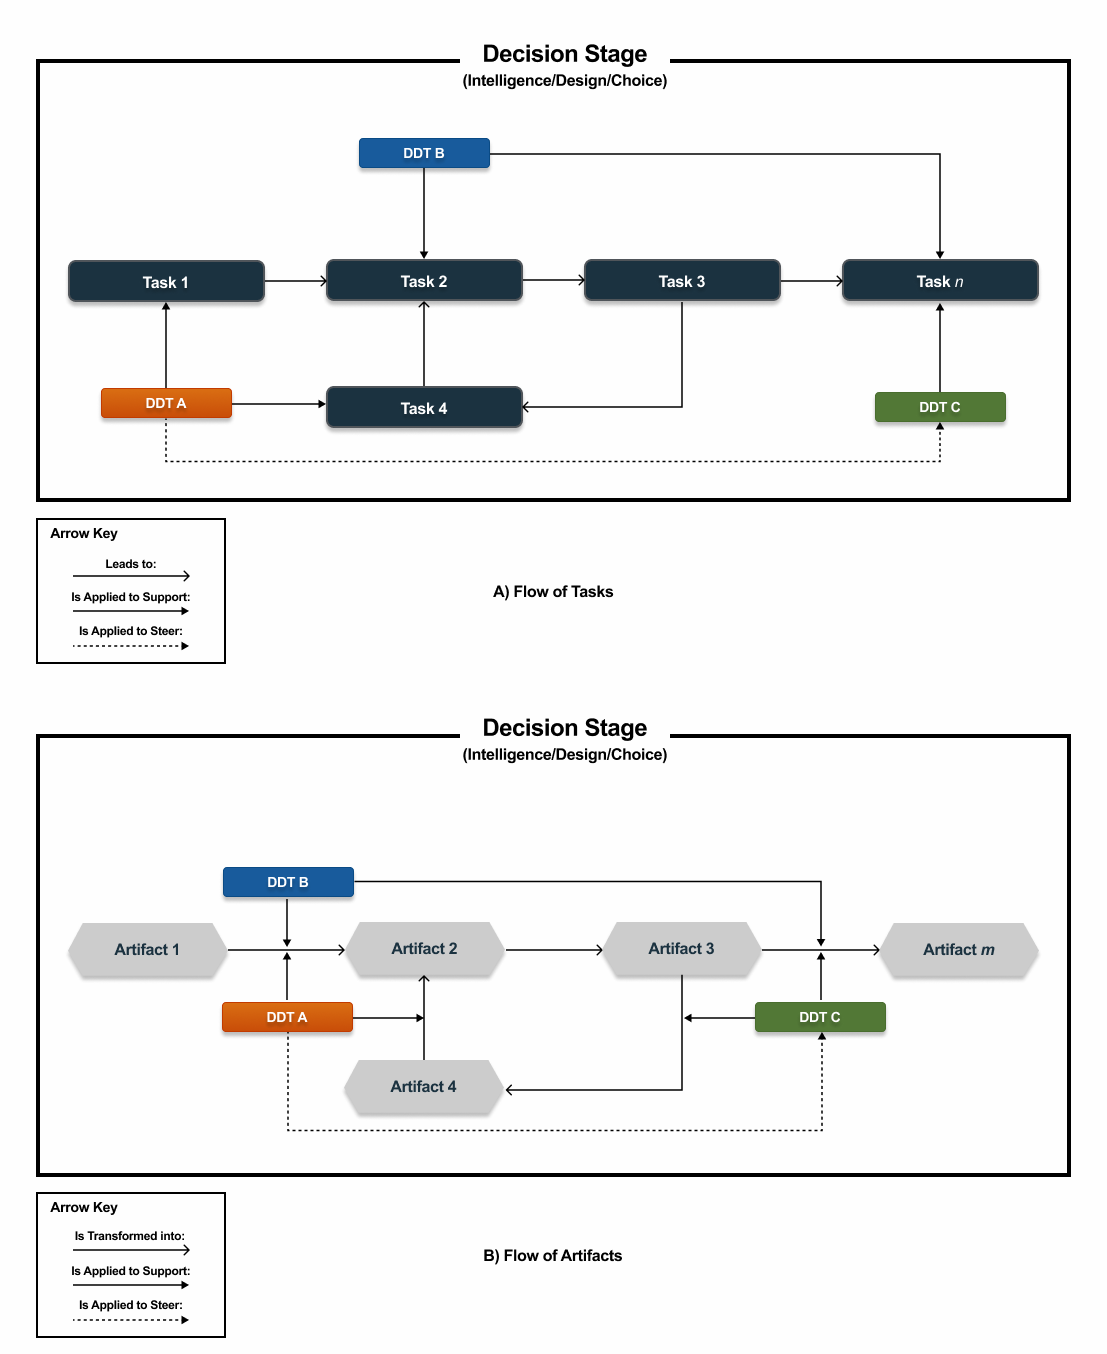
\includegraphics[width=6in]{Figures/DDTOrchestrationFramework.png} % ≤ 6 inches wide
    \caption[A visual model for our proposed orchestration framework]{A visual map for orchestration of DDTs A, B, and C towards supporting: A) the flow of tasks, and B) the flow of artifacts within a decision stage. In (A), DDT A is applied to support Tasks 1 and 4, while DDT B supports Tasks 2 and \textit{n}, and DDT C only supports \textit{n}. In (B), both DDT A and DDT B support generation of Artifact 2, whereas both DDT B and DDT C support generation of Artifact \textit{m}. Generation of Artifact 4 is only supported by DDT C.}
    \label{DDTOrchestrationModel}
\end{figure}
The flow of tasks or artifacts within each decision stage was founded on the grounds of a pre-existing process model that describes the common steps taken in that particular stage with extended details compared to Simon's model, aiding us with guided exploration of the state-of-the-art application of data-driven tools to support the activities throughout the stage. The visual analytics (VA) framework, causal graph construction process from Kling~\cite{kling2025co}, and MCDM-based alternative evaluation and selection served as the foundational models for the intelligence, design, and choice stages, respectively. Therefore, an orchestration map for every decision stage can be generated that follows one of the patterns in Figure ~\ref{DDTOrchestrationModel}.
\clearpage
% For example, the visual analytics (VA) framework describes the activities that are commonly performed in the intelligence stage of the decision-making process; therefore, we will provide a synthetic workflow describing how and towards serving which particular activities throughout the visual analytics process, different data-driven tools (e.g., ML and natural language models) in previous research publications have been employed. For example, during the intelligence stage, interactive visualization helps DMs explore different aspects of the data and generate new data-driven hypotheses, while statistical analysis methods enable them to validate the previous hypotheses formed as a result of interaction with visualized data. 
% To generate a workflow for orchestration of multiple DDTs in a stage, we investigate the stage-relevant practical use-cases of such tools in a set of relevant publications and synthesize them in the context of the initial process model.   
\subsubsection{Our Proposed Orchestration Workflow of Data-Driven Tools for Intelligence Stage}
The synthesis of the studies presented in Section ~\ref{ExistingResearchIntelligence} guides us towards an effective Intelligence-stage orchestration workflow combining visualization (VIZ), machine learning (ML), traditional statistics (TS), and language models (NLMs) into a closed-loop system visualized in Figure ~\ref{IntWorkflow} that follows the flow of artifacts pattern in Figure ~\ref{DDTOrchestrationModel}. As shown in the figure, discussed DDTs can enhance the sense-making process via the following steps:\par
\textbf{Step 1. Data Ingestion and Preprocessing:} Raw structured/unstructured data is preprocessed and prepared for later visual encodings with the aid of ML techniques and NLP models:\par
{
\setlength{\leftskip}{0.5cm}
\noindent•	\textbf{Scenario 1.1.} ML algorithms automate data transformation, remove noisy data, impute missing values, select important features, reduce the dataset’s dimension, recognize latent patterns and structures, and detect anomalies in structured data.\par
\noindent•	\textbf{Scenario 1.2.} ML algorithms extract features, cluster and model topics, reduce data dimensions, perform semantic filtering, and recognize named entities in unstructured data. Ontology(rule)-based NLP models and LLMs can also be employed to classify topics according to expert-defined rules and summarize a large volume of unstructured information.\par
}
The user can also steer and refine these ML algorithms’ parameters with the aid of interactive visualization idioms (e.g., sliders, switches). The algorithms’ structure and performance can also be tracked and explained by visual graphs (e.g., saliency maps and feature importance plots).\par
\textbf{Step 2. Visual Encoding:} Preprocessed data is mapped into a default interactive visual representation such as a dashboard, consisting of multiple specified views (e.g., networks, timelines, heatmaps) that are coordinated, linked, or juxtaposed.\par 
\textbf{Step 3. Visual Data Exploration:} Users explore the visualized data through interactive idioms and linking views. Natural-language-based visual and data queries can assist users in building the view and exploring the data portion of their interest. The data or view to be explored can also be recommended by embedded ML models or rule-based AI systems in general.\par   
\textbf{Step 4. Insight Generation}: By interactively exploring visual information, users gain new insights about the data. This insight generation can also be boosted with the aid of LLMs’ semantic reasoning and narrative generation power, as well as additional analytical tools such as descriptive statistical measurements (e.g., univariate central tendency analysis, multivariate regression analysis, etc.).\par  
\textbf{Step 5. Hypothesis Generation and Testing:} As users form new hypotheses about the data based on their current knowledge, they may do either of the following scenarios:\par
{
\setlength{\leftskip}{0.5cm}
\noindent•	\textbf{Scenario 5.1.} Users directly run a formal statistical test to validate the hypothesis, leading to an instant result that contributes to their current knowledge about the data. Inferential statistics techniques, such as analysis of variance (ANOVA) and p-value adjustment methods (e.g., Benjamini-Hochberg), can play a role in facilitating this process.\par
\noindent•	\textbf{Scenario 5.2.} Users visually analyze the data to see whether the visualized information supports their hypothesis. This means that users return to the visual data exploration step, while some interactive-visualization-based methods (e.g., \textit{Lineup protocol}) might particularly be used to help users systematically validate their hypothesis with an accuracy comparable to formal tests.\par
}
\textbf{Step 6. (Decision) Problem Identification:} Throughout this iterative cycle of data exploration, insight gathering, and hypothesis testing, users eventually identify a problematic pattern, anomaly, or business gap that drives them to make a decision about it.\par
The above workflow for orchestration of different DDTs inside the VA-aided intelligence stage provides the foundation for integrative design of tools from every DDT class for every step of the sense-making process. A VA system that effectively enhances users’ sense-making should embrace these integrated solutions to adapt to a variety of users’ analytical needs and expectations throughout this iterative process.
\begin{landscape}
\begin{figure}
    \centering
    % Ensure figure width fits within SFU margins
    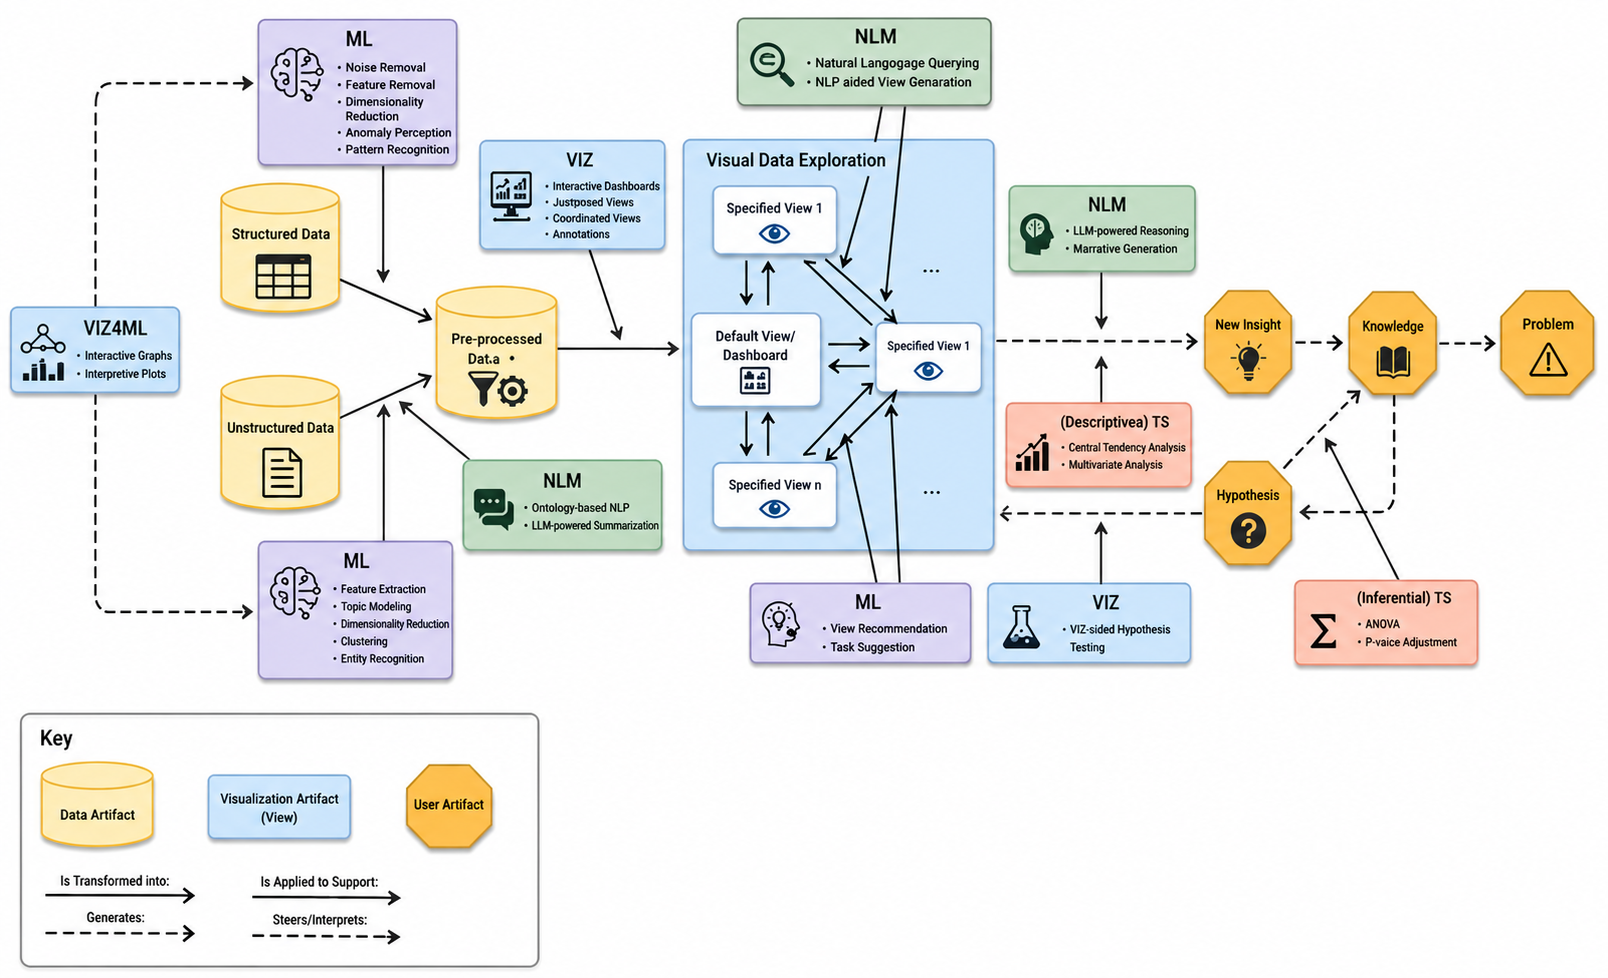
\includegraphics[width=8in]{Figures/IntelligenceWorkflow.png} % ≤ 6 inches wide
    \caption[An orchestration workflow for the intelligence stage]{Our proposed visual-analytics-based workflow for orchestration of data-driven tools for the intelligence stage of decision-making process}
    \label{IntWorkflow}
\end{figure}
\clearpage
\end{landscape}

\subsubsection{Our Proposed Orchestration Workflow of Data-Driven Tools for Decision Design Stage}
Synthesizing the summaries of the studies presented in the section ~\ref{ExistingResearchDesign} in the context of the causal graph construction and validation process (adopted from Kling~\cite{kling2025co}) leads to the following workflow as an attempt to orchestrate the DDTs supporting the decision design stage:\par
\textbf{Step 1. Decision Problem Formulation:} Decision goal(s), criteria/outcome(s), and lever(s) are identified. Decision stakeholders generate alternative solutions during brainstorming sessions. \par
\textbf{Step 2. Intermediate and Exogenous Factors Identification:} The most influential factors that mediate or confound the achievement of decision objectives via implementing alternative solutions are discovered.\par
\textbf{Step 3. Causal Interactions Identification and Causal Graph Construction:} Decision stakeholders specify \textbf{\textit{how}} (i) implementing each solution and (ii) exogenous factors causally affect the decision outcomes via intermediate variables. An initial version of the causal graph is built.\par
The LLMs can be engaged to support these three steps by gathering useful information from external (online) sources and reasoning about the involved causal factors and their interactions.\par
\textbf{Step 4. Informing Causal Relationships:} Decision stakeholders assign the perceived causal strength and an SCM function to every relationship (edge) in the causal graph's current version.\par
{
\setlength{\leftskip}{0.5cm}
\noindent• \textbf{Scenario 4.1.} The SME directly specifies an SCM function if it is already known. This is particularly the case when the stakeholders are almost certain about the existence of a causal relationship between the two variables.\par
\noindent• \textbf{Scenario 4.2.} An SCM function is learned from the data using an ML model of the experts' choice (e.g., \textit{linear/logistic regression}).\par
}
\textbf{Step 5. Causal Assumption Validation:} Assumed causal relationships are cross-checked with the data (if accessible). Invalid relationships are redirected back to Step 3 or 4 for re-investigation and revision.\par
{
\setlength{\leftskip}{0.5cm}
\noindent• \textbf{Scenario 5.1.} Decision stakeholders and SMEs visually inspect the multidimensional data to discover whether an observed pattern in the data validates the SCM. Contingency tables are effective VIZ tools towards this purpose.\par
\noindent• \textbf{Scenario 5.2.} Statistical measurements, tests, and procedures are calculated and run to identify invalid causal assumptions or SCM functions. Most specifically, FDCR-adjusted Benjamini-Hochberg p-values (proposed by Kling~\cite{kling2025co}) indicate the statistical significance of presumed relationships relative to their perceived strengths (declared by SME in Step 4).\par
}
As also shown in Figure ~\ref{designWorkflow} that also follows the flow of artifacts pattern in Figure ~\ref{DDTOrchestrationModel}, the above steps are iteratively taken until all SCMs are validated, and the final version of the causal graph is achieved, in which every (dependent) child node is mathematically mapped to its parents. Such a mathematically informed causal graph provides the foundation for evaluating solutions' performance and prediction of their outcomes, as the central activity in the choice stage.\par
\begin{landscape}
\begin{figure}
    \centering
    % Ensure figure width fits within SFU margins
    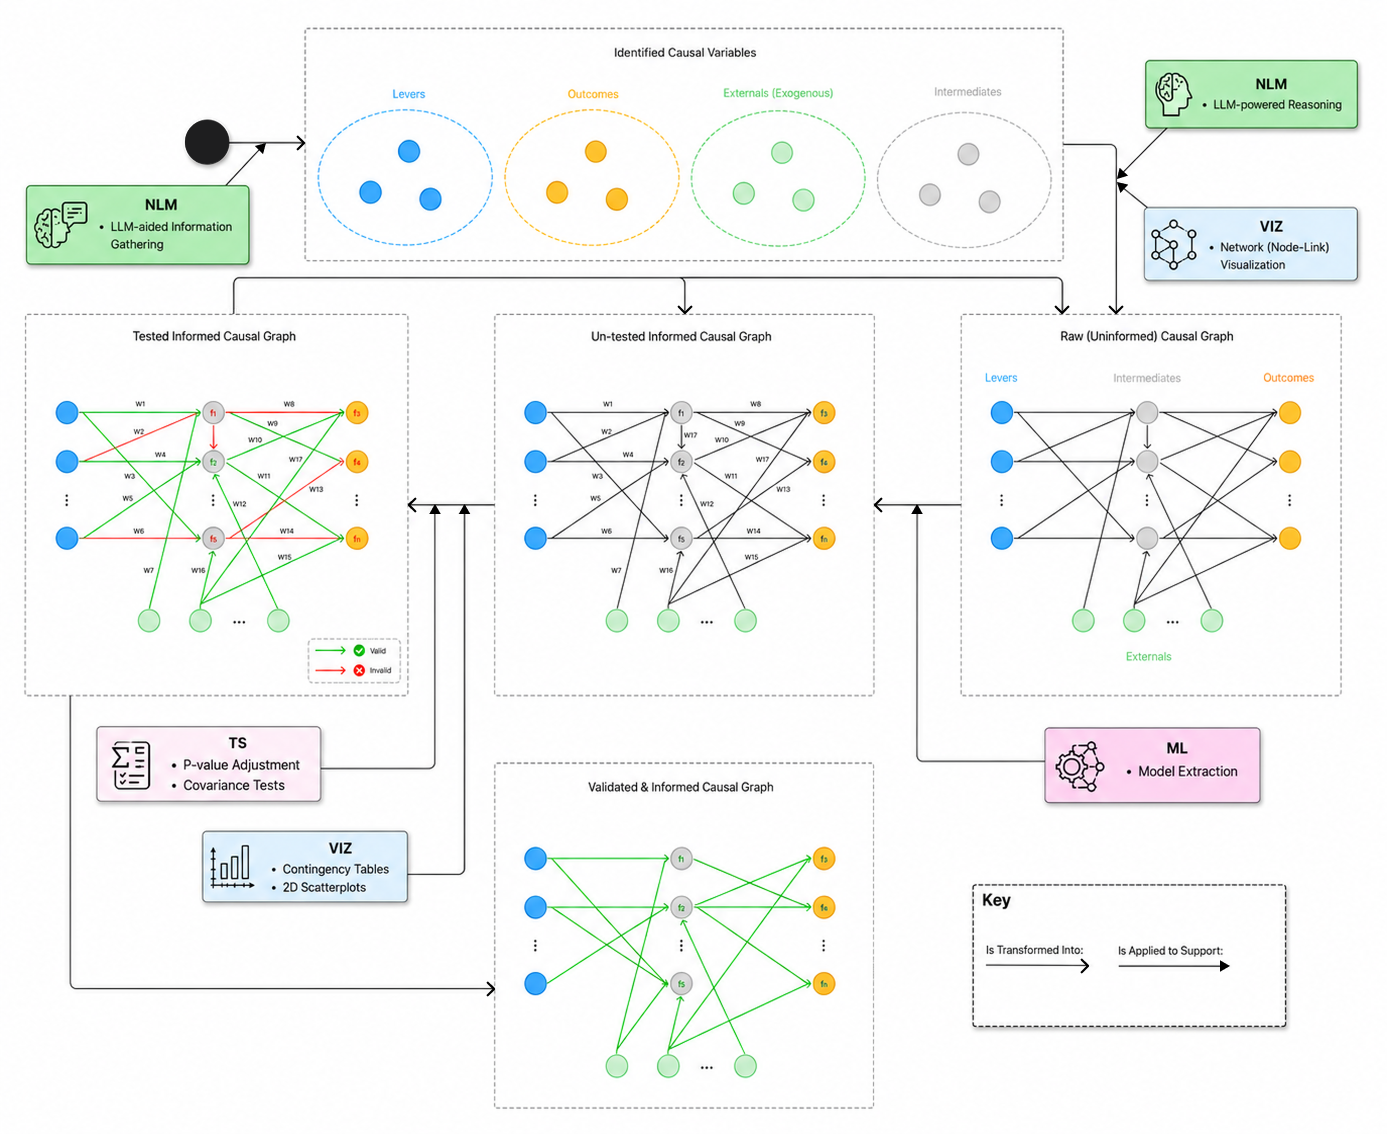
\includegraphics[width=7in]{Figures/DesignWorkflow_ArrowsAmplified.png} % ≤ 6 inches wide
    \caption[Orchestration workflow for the decision-making design stage]{Our proposed causal-graph-construction-based workflow for orchestration of data-driven tools in the decision-making design stage.}
    \label{designWorkflow}
\end{figure}
\clearpage
\end{landscape}

\subsubsection{Our Proposed Orchestration Workflow of Data-Driven Tools for Choice Stage}
The results of the presented studies in the section ~\ref{ExistingResearchChoice} can be synthesized into the following workflow, orchestrating all classes of data-driven tools applications to effectively support the main activities in the choice stage of the decision-making process:\par
\textbf{Step 1. Decision Model Initialization:} An initial set of values for external variables is provided to the pre-developed causal decision model.\par
\textbf{Step 2. Optimal Solution Exploration:} Plausible solutions to the decision problem are evaluated and explored, so that an optimal or satisfactory solution to the decision problem is discovered.\par 
{
\setlength{\leftskip}{0.5cm}
\noindent•	\textbf{Scenario 2.1.} DM users evaluate the outcomes of every solution directly by setting a specific value for every decision lever and observing the generated value for every outcome interactively. This outcome prediction is powered by a computation engine that utilizes simulation, propagation, or ML-aided prediction, while the computed values are visualized in an interactive dashboard. An optimal or satisfactory solution might be discovered via these interactions with the computational decision model.\par
\noindent•	\textbf{Scenario 2.2.} DM users prompt the model to mathematically discover a set of values that makes the outcomes retain the optimal values.\par
}
{
\setlength{\leftskip}{1cm}
\noindent•	\textbf{Scenario 2.2.1.} DM users explicitly provide their preference information to the model as a set of numerical weights for the outcomes, or in a hierarchical structure to make the optimization algorithm directly find a single optimal solution (i.e., \textit{priori} preference input model).\par
\noindent•	\textbf{Scenario 2.2.2.} DM users skip the preference information, making the optimization algorithm generate a continuous or discrete set of Pareto optimal solutions as candidate final solutions (i.e., \textit{posteriori} preference input model).\par
\noindent•	\textbf{Scenario 2.2.3.} DM users provide their preferences interactively in the course of the optimization process, steering the optimization algorithm towards the preferred regions of the Pareto front curve to finally reach a single optimal solution (i.e., \textit{interactive} preference input model). Such an interactive preference elicitation model may involve interactive VIZ for selection of the preferred optimization path in every iteration of the optimization algorithm.\par
}
\textbf{Step 3. Solution Selection:} In case scenarios 2.1 and 2.2.2 take place, DM users compare different non-dominated solutions to select the most desired one.\par
{
\setlength{\leftskip}{0.5cm}
\noindent•	\textbf{Scenario 3.1.} DM users visually compare the performance of different solutions on every criterion or in general. VIZ structures and techniques, such as juxtaposed graphs, grouped or stacked bar charts, facilitate solutions' comparison.\par
\noindent•	\textbf{Scenario 3.2.} DM users employ a multi-criteria decision-making (MCDM) method to systematically choose the most desired solution.\par
}
{
\setlength{\leftskip}{1cm}
\noindent•	\textbf{Scenario 3.2.1.} If the set containing all non-dominated solutions is discrete, DM users employ a multi-attribute decision-making (MADM) method (e.g., AHP, TOPSIS) to select an alternative solution that performs the best on aggregate among all the alternatives. This requires users to express their preferences in terms of direct weights, hierarchical goals, or pairwise comparisons.\par
\noindent•	\textbf{Scenario 3.2.2.} If the set containing all non-dominated solutions is continuous (as a result of Pareto optimal discovery in scenario 2.2.2, the user employs a multi-objective decision-making (MODM) method to discover an optimal solution delivering the best projected performances in all criteria on aggregate across all Pareto optimals. Depending on the selected MODM algorithm, the DMs' preferences are specified before the algorithm is run, or over its course of progress interactively and continuously.\par
}
\textbf{Step 4. Sensitivity and Robustness Analysis:} The performance of the optimal solution discovered is tested with different possible values for the model's external variables to examine whether it remains optimal or satisfactory in different exogenous conditions. If the solution performs poorly under new conditions, the users return to step 2 to discover and select the optimal solution under the new conditions. \par  
\textbf{Step 5. Final Choice:} A reliable and satisfactory solution that performs solidly over a range of possible environmental scenarios is selected as the final choice.\par
The above synthesized workflow has also been illustrated in Figure ~\ref{choiceWorkflow} following the flow of tasks pattern in Figure ~\ref{DDTOrchestrationModel}. The artifacts generated as a result of every task accomplishment have also been shown by violet hexagons in the same figure. While we did not investigate a particular case in which LLMs were employed to assist DMs with any of the above workflow's activities, some publications (e.g., ~\cite{handler_large_2024}) have called for further studies on the opportunities and challenges that the application of LLMs during the choice stage of the decision-making process presents.\par

\begin{figure}
    \centering
    % Ensure figure width fits within SFU margins
    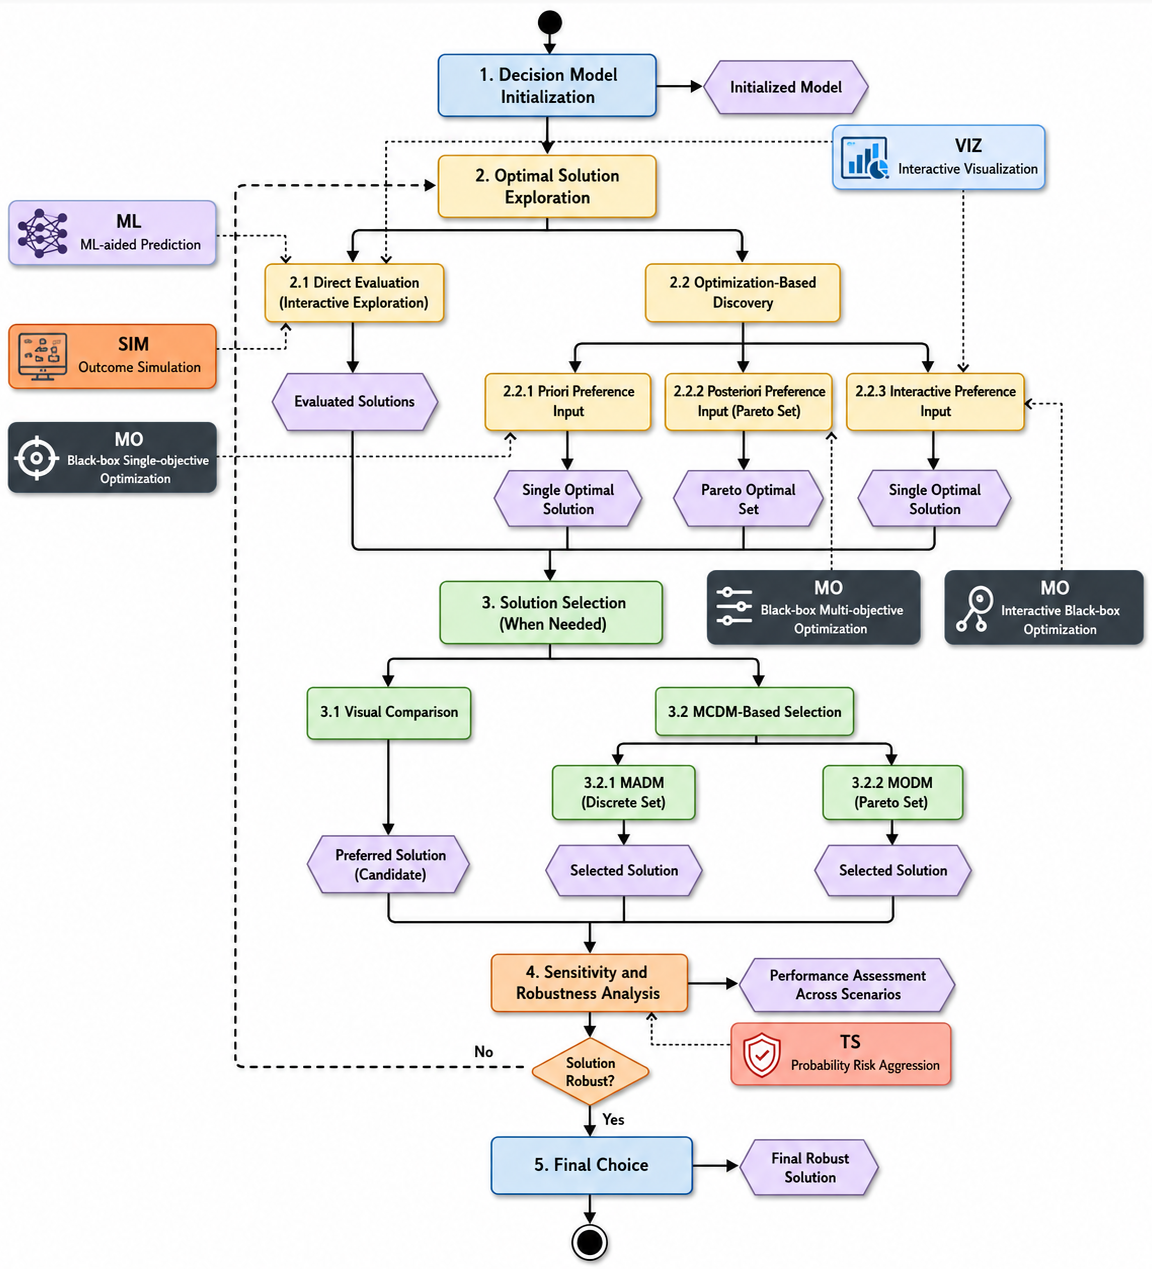
\includegraphics[width=6in]{Figures/ChoiceWorkflow.png} % ≤ 6 inches wide
    \caption[Orchestration workflow for the decision-making choice stage]{Our proposed mathematical optimization and MCDM-based workflow for orchestration of data-driven tools in the decision-making choice stage.}
    \label{choiceWorkflow}
\end{figure}
\clearpage
\subsection{A Human-Data-Task-Centered Framework for Integration of Data-Driven Tools}
Unlike orchestration, integration of DDTs within a single solution is a context-dependent process that requires DSS designers to first select and specify a single tool from every DDT class of tools mapped to a stage, before configuring the logical dependencies and interaction points between all the tools selected from different DDT classes.
The human-data-task-centered integration of DDTs into a unified solution capable of assisting the DM in accomplishing a wide range of tasks within a particular stage is affected by factors such as \textit{decision type}, the type and structure of data, and the DM's personal and cognitive characteristics. To systematically produce such a human-centric, flexible, and cross-technology decision support solution, we propose a three-layer \textit{bottom-up} framework as illustrated in Figure ~\ref{DDTIntegration}, consisting of a \textbf{Selection} layer, a \textbf{Customization} layer, and an \textbf{Integration} layer. In the selection layer, for every DDT category mapped to the stage (e.g., DDT A), a tool from the basic set of more recognized tools (e.g., Tool A1 to Tool A3) inside that particular DDT is selected as the main design option. In the customization layer, the practical design of selected tools’ constituting elements is specified in more detail. Finally, in the integration layer, the selected and customized tools from all DDT classes are assembled into an integrated solution to be used by DMs for accomplishing the different activities and tasks throughout the decision stage.\par
At an abstract level, this integration process is taken to generate a \textit{DSS architecture} that incorporates tools from different DDTs, aiding the DM in performing an abstract decision task or activity. Data preprocessing during the intelligence stage, for instance, is an activity that can be supported by different ML tools, NLP technologies, LLMs, and data visualization (VIZ) that can altogether be assembled in a \textit{data preprocessing pipeline} within a hypothetical DSS. At a detailed level, the integration process is taken to produce a solution module only to optimally accomplish a data-level task. For example, \textit{identification of correlation} between two data variables involves both data visualization (VIZ) and traditional statistical analysis (TS), making the designer select a specific tool from each involved DDT (e.g., scatterplots from VIZ, and Pearson's $r$ correlation coefficient from descriptive TS), customize or specify each selected tool (e.g., differentiating the plots' color from the chart's background color in the scatterplot, adjust the axes' ticks, etc.), and integrate both into a final solution (e.g., visualizing the Pearson's $r$ value on top of the scatterplot). A stage-level integrated solution can be implemented by further integration of these integrated solution modules for the data-level tasks.\par
\begin{figure}
    \centering
    % Ensure figure width fits within SFU margins
    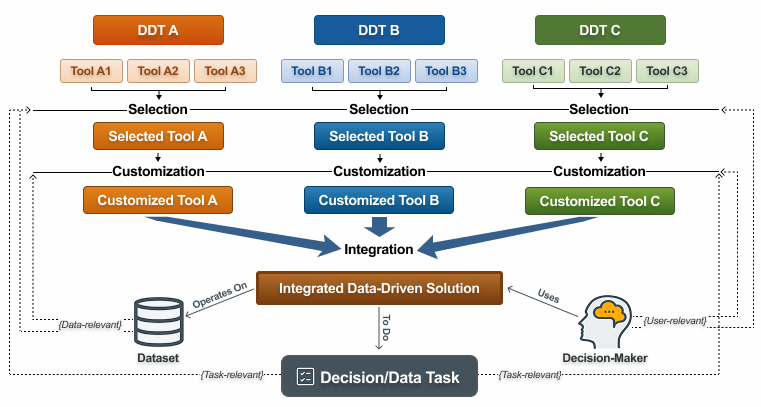
\includegraphics[width=6in]{Figures/ThreeLayerIntegration.png} % ≤ 6 inches wide
    \caption[Proposed framework for integration of DDTs]{Our proposed human-data-task-centered framework for integration of data-driven tools (DDTs) to effectively support a task in the decision-making process.}
    \label{DDTIntegration}
\end{figure}
The selection, customization, and integration (SCI) are all accomplished according to research-based considerations that are related to either the task’s nature and context, the DM’s humanistic properties and cognitive capacities, or the dataset’s structure. We refer to such considerations as \textit{rules}, and classify them in three groups of \textit{clinical (task-relevant), data-relevant,} and \textit{user-relevant}, all rooted in academic findings. Clinical rules are those that have been derived from the clinical observations of the methods’ performance in accomplishing data tasks based on the objective performance criteria. For example, prior studies have shown that data visualization users perform more accurately and efficiently in finding anomaly tasks when using bar charts over pie charts, line charts, and flat data tables ~\cite{saket2018task}. Data-relevant rules set boundaries on each DDT’s comprised methods to be selected for supporting the data task at hand according to the data types, size, dimensionality, and quality of the target dataset. An example of a data-relevant rule is the better performance and stability of the XGBoost method over the rest of the supervised machine-learning methods for large datasets ~\cite{cao2022systematic}. User-relevant rules force humanistic considerations to be taken into account when selecting, customizing, and synthesizing data-driven methods. Looking back at data visualization as an example, the studies have shown that users with lower spatial abilities should be exposed to 2D charts over 3D versions, as the latter demand enormous levels of visuospatial cognitive processing ~\cite{chikha2021effect}. Every single rule clause is not necessarily unique for a task, the DDTs assigned to the task, nor the framework layer (that can either be selection, customization, or integration) wherein the analysis happens. For instance, the clinical and cognitive superiority of aligned bar charts over the stacked ones ~\cite{talbot2014four, cleveland_graphical_1984} as a clinical and user-relevant rule is considered in configuring the design of an integrated solution for any task that involves data visualization DDT (and when a bar graph is selected as the base visualization tool).\par
The strong dependence on the characteristics of the decision-making problem, together with the large number of data-level tasks, data-driven tools, and considerations governing their effective application, makes it impractical to instantiate the proposed integration framework for every task across the entire decision-making process. Consequently, a comprehensive task-by-task instantiation falls beyond the scope of the present work. Future research should instead focus on developing systematic and proactive roadmaps that guide the SCI process of data-driven tools for specific activities within the broader decision-making process. These roadmaps can be represented as decision flows, such as the one illustrated in Figure ~\ref{IntegrationFlowchart}, where each decision point (i.e., diamond) corresponds to a specific category of design rule (i.e., task-related, user-related, or data-related). These rules guide the selection of the most appropriate data-driven tool or design alternative for supporting the activity at hand. As illustrated in the figure, a particular variant from the available alternatives within DDTA, DDTB, or DDTC may be identified as the most suitable option when the corresponding decision criteria or contextual conditions are satisfied.\par
\begin{figure}
    \centering
    % Ensure figure width fits within SFU margins
    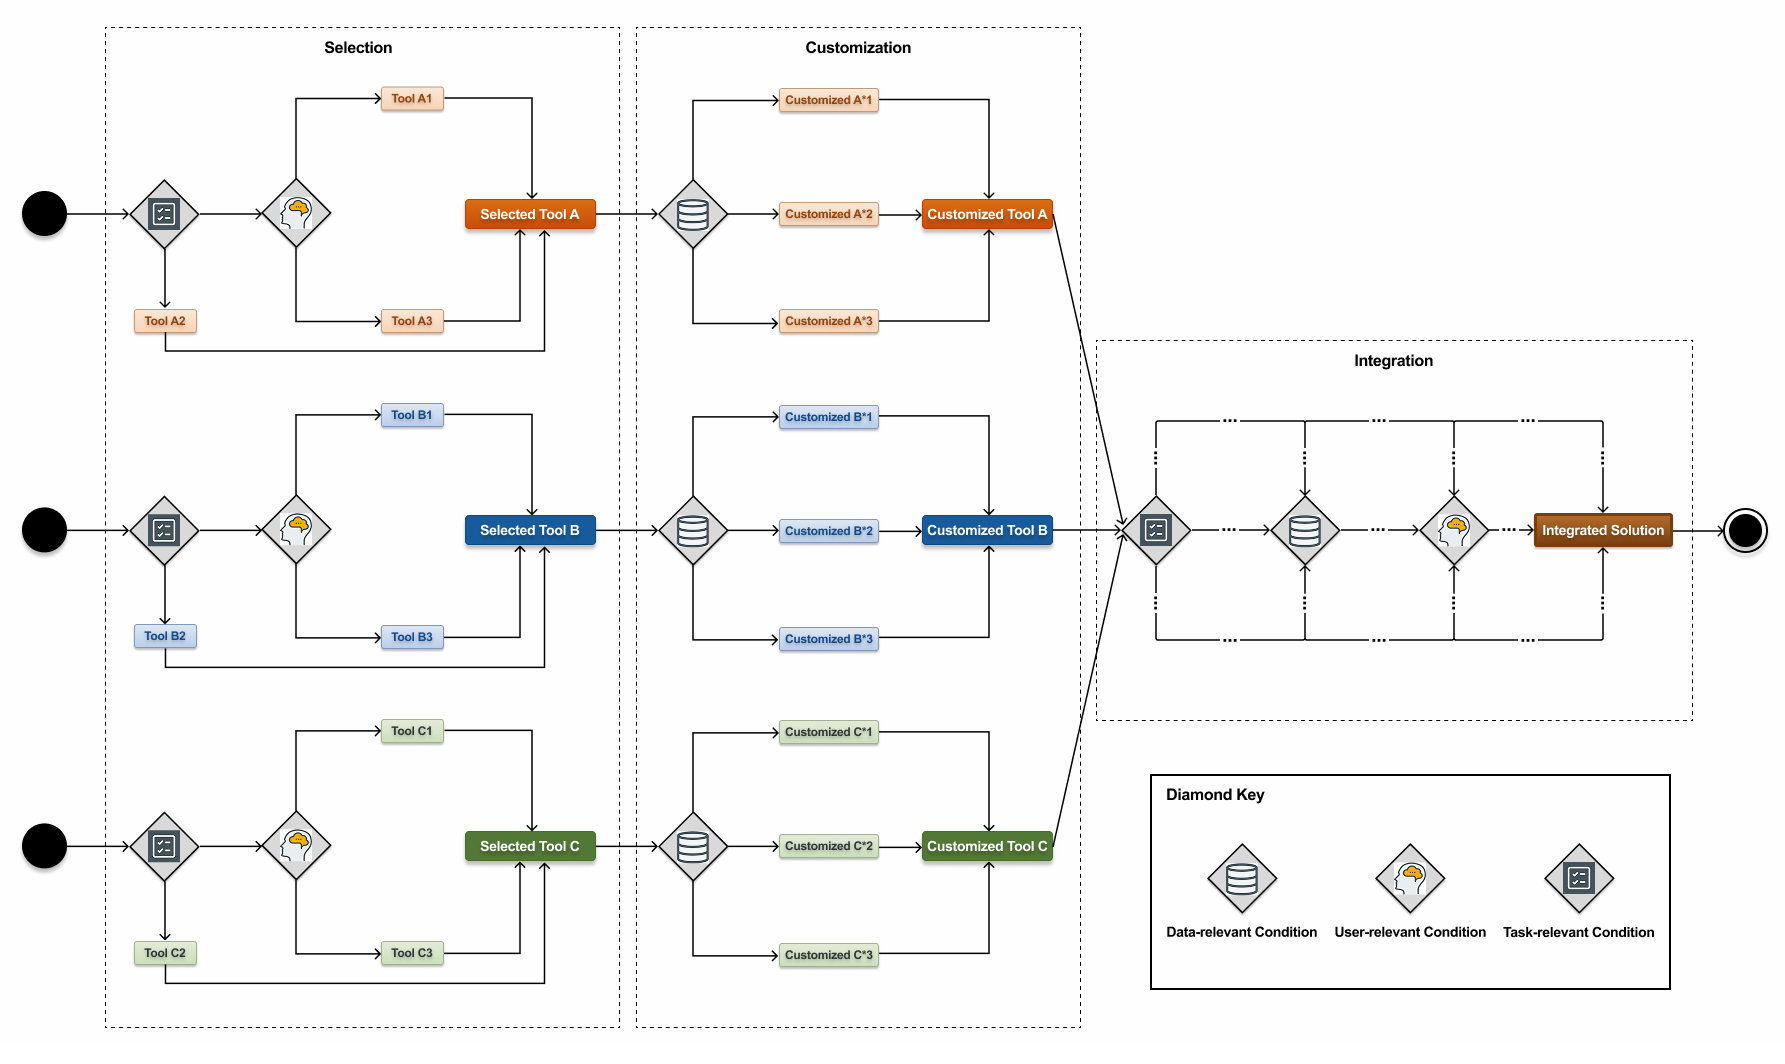
\includegraphics[width=6in]{Figures/IntegrationFlowchart.png} % ≤ 6 inches wide
    \caption[A conceptual decision flow example for SCI process]{A conceptual decision flow example for selection, customization, and integration (SCI) of the most suitable tools and design approaches for three DDT A, B, and C, guided by multiple conditions representing task-relevant, data-relevant, and user-relevant factors.}
    \label{IntegrationFlowchart}
\end{figure}
The decision logic underlying the SCI process of data-driven tools is likely to be considerably more complex than the simplified representation shown in Figure ~\ref{IntegrationFlowchart}. For example, \textit{information filtering}—a data-level task identified in the taxonomies proposed by Amar et al.~\cite{amar_low-level_2005} and Munzner~\cite{munzner_visualization_2015}—can be supported through a wide range of data visualization techniques in combination with natural language querying (NLQ), as illustrated by the orchestration workflow of the intelligence stage (Figure ~\ref{IntWorkflow}). Designing and integrating an effective solution for this task requires consideration of numerous task-related, data-related, and user-related factors. Collectively, these factors guide designers toward the most appropriate combination of technologies and design alternatives for supporting the task, as conceptually illustrated in Figure ~\ref{FilterInfo_IntegrationFlow}.
\begin{figure}
    \centering
    % Ensure figure width fits within SFU margins
    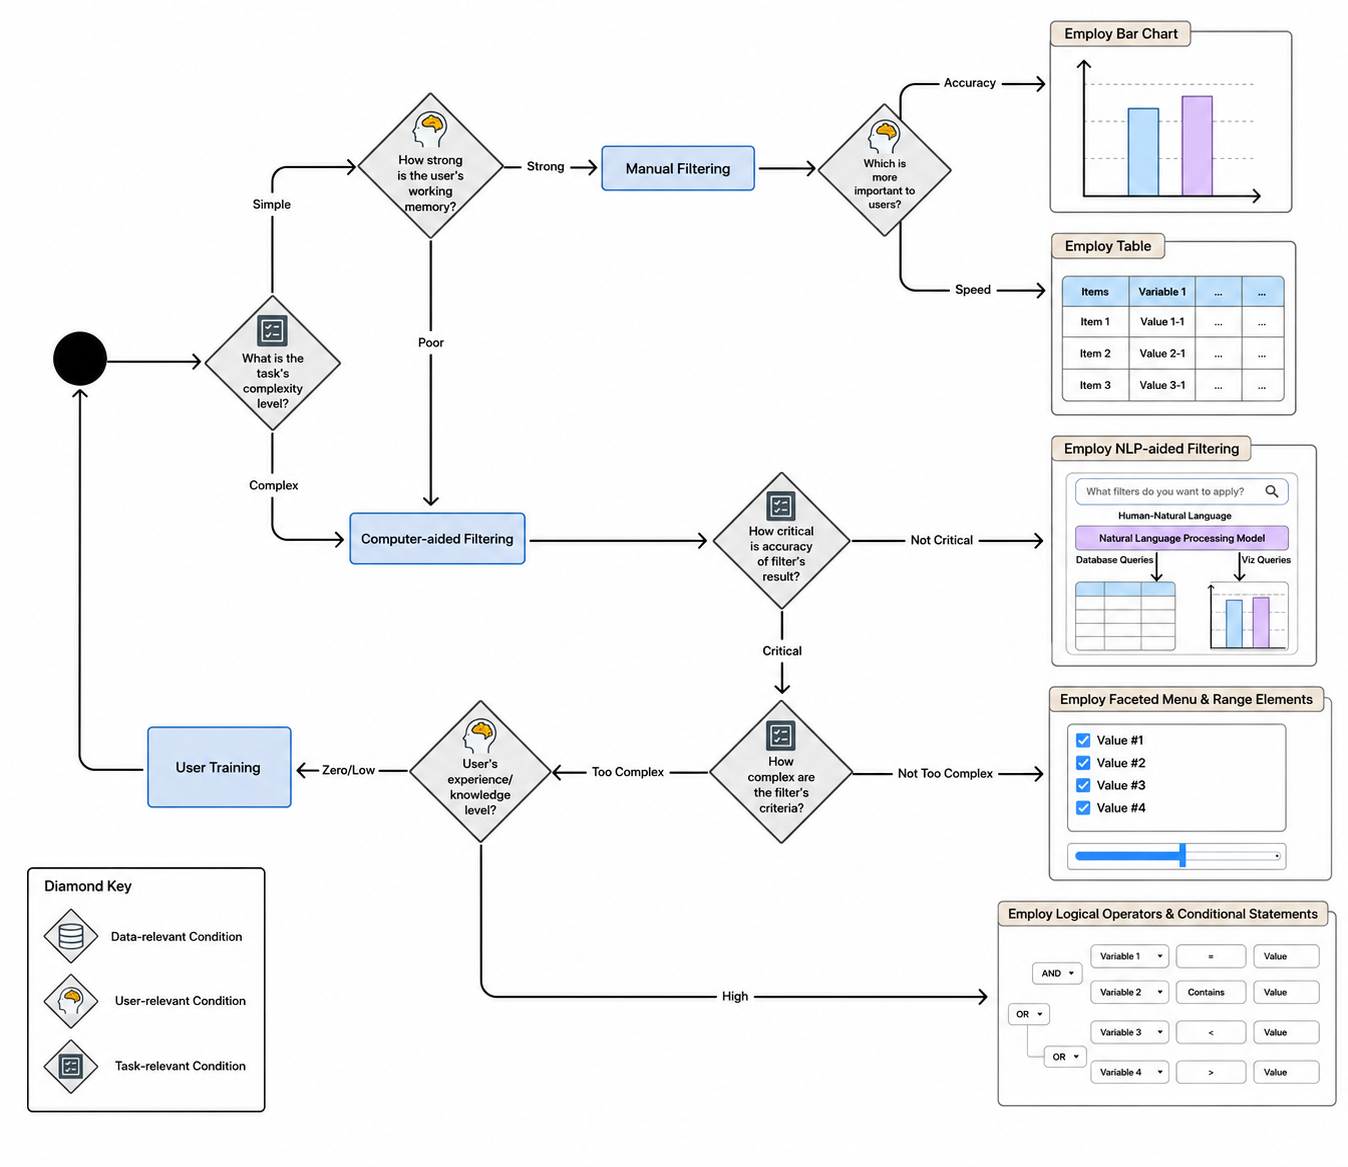
\includegraphics[width=6in]{Figures/FilterInformation_IntegrationWorkflow.png} % ≤ 6 inches wide
    \caption[A decision flow example for guiding the SCI process for information filtering task]{A decision flow for determining the most suitable tool and design approach for the information filtering task according to multiple task-relevant (e.g., filtering criteria complexity) and user-relevant (e.g., the strength of working memory, and knowledge/experience level) factors.}
    \label{FilterInfo_IntegrationFlow}
\end{figure}
As illustrated in Figure ~\ref{FilterInfo_IntegrationFlow}, both task-related factors (e.g., the complexity of the filtering criteria) and user-related factors (e.g., users' knowledge and level of expertise) influence the selection of the most appropriate tool or design approach. For instance, when a filtering task is sufficiently simple to be performed manually using a static visualization, bar charts may be preferable to data tables for users who prioritize the accuracy of filtering outcomes over execution speed. Conversely, for visually filtering small datasets, data tables have been shown to outperform graphical representations, including bar charts, in terms of task completion time, as demonstrated by the empirical findings ~\cite{saket2018task}. Conversely, when the filtering task is complex or exceeds the user's working memory capacity, computer-assisted filtering becomes essential. In such cases, interactive visualization techniques and user interface controls are required to enable the specification of filtering criteria. Among the available computer-assisted approaches, the NLP-based filtering architecture proposed by Zhang et al.~\cite{zhang2024natural} may serve as an appropriate default solution in applications where absolute filtering accuracy is not a primary requirement. However, when maximizing filtering accuracy is critical, explicit user-controlled inputs, such as text fields, selection boxes, and slider controls, should be employed to ensure the precise specification of filtering criteria.

The complexity of the filtering criteria further influences the choice of interaction mechanisms. When the criteria are relatively simple, faceted search interfaces and range-selection controls (e.g., sliders) are generally sufficient. In contrast, complex filtering tasks require more expressive interaction techniques, including conditional expressions and logical operators, to enable the accurate formulation of filtering rules. The effective use of these advanced interaction mechanisms, however, often presupposes a certain level of user expertise and domain knowledge. Consequently, when such competencies are lacking, appropriate user training or interface guidance should be provided to ensure the effective use of the filtering system.

Comparable decision roadmaps can likewise be developed to support the design of integrated solutions for activities beyond the intelligence stage. For example, the selection of an appropriate optimization or MCDM method for identifying optimal solutions to a formulated decision problem illustrates how characteristics of the problem can systematically guide the design of an integrated decision support solution for the choice stage. As indicated by the orchestration workflow for the choice stage (Figure ~\ref{choiceWorkflow}), when the decision-maker's preferences are unavailable or cannot be elicited a priori, the search for Pareto-optimal solutions should be performed using a black-box MOO algorithm. Given the diversity of available black-box MOO approaches—including direct search methods (e.g., MADS and GPS), evolutionary algorithms, and surrogate-assisted optimization methods—the most appropriate technique can be selected by evaluating a sequence of conditions, as conceptually illustrated in Figure ~\ref{MOOSelectionFlow}.\par
\begin{figure}
    \centering
    % Ensure figure width fits within SFU margins
    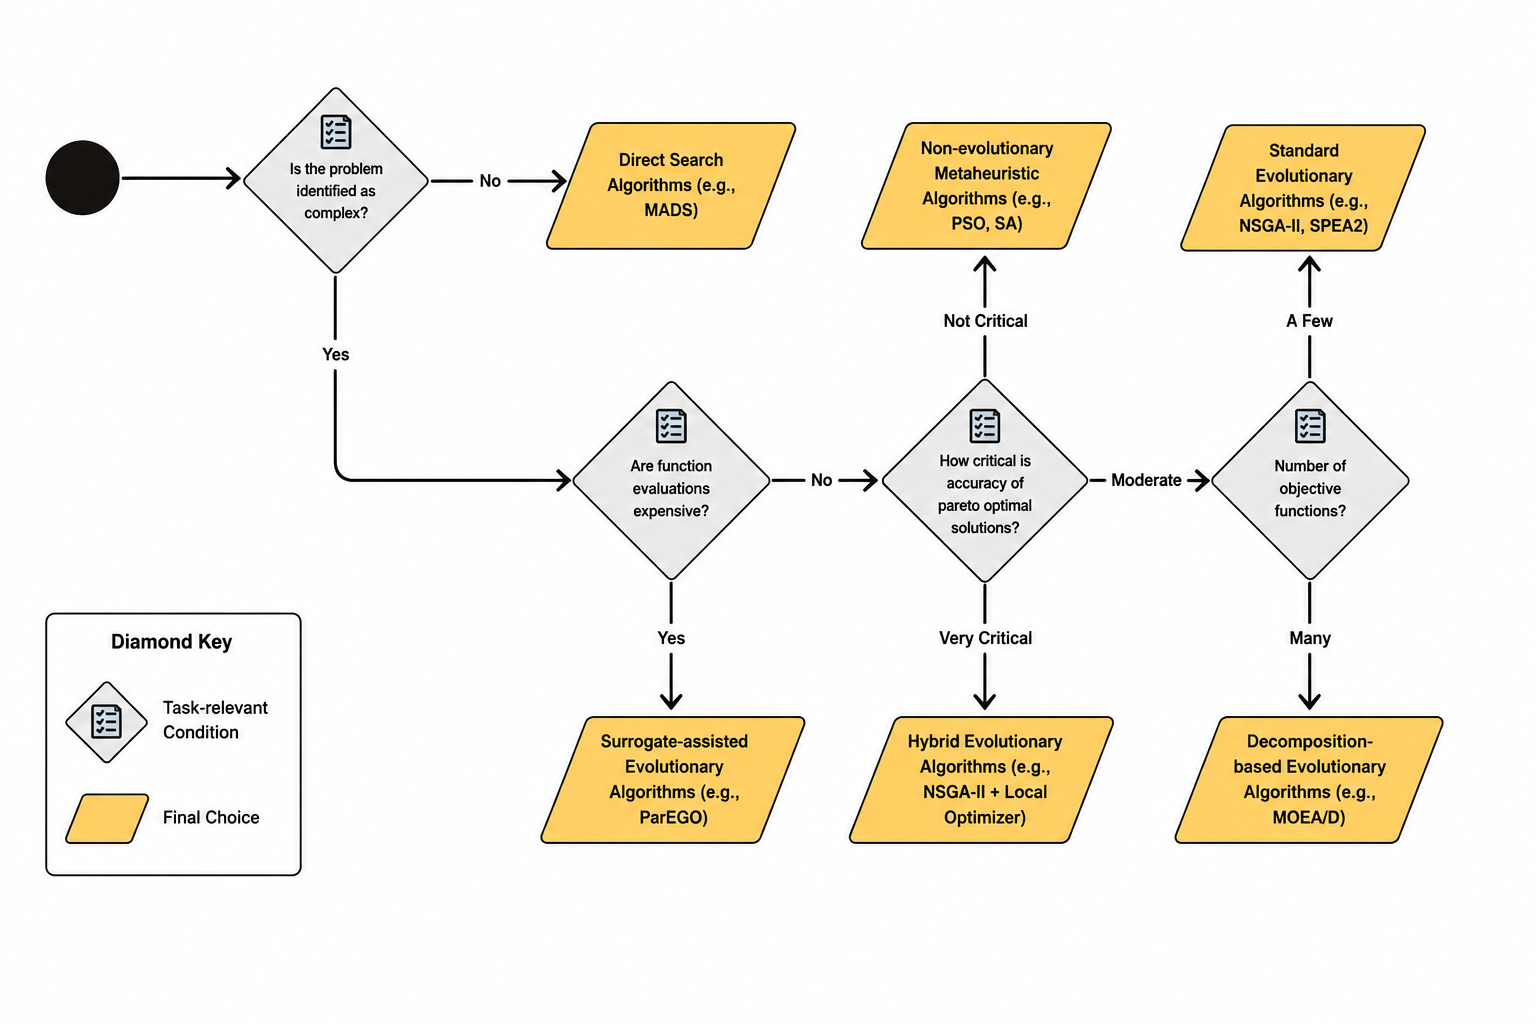
\includegraphics[width=6in]{Figures/MOOSelectionFlow.png} % ≤ 6 inches wide
    \caption[A decision flow example for selection of the most suitable class of black-box MOO methods]{A decision flow for determining the most suitable black-box multi-objective optimization (MOO) class of methods according to multiple task-relevant factors (e.g., computational cost of objective function evaluations).}
    \label{MOOSelectionFlow}
\end{figure}
As discussed in Section ~\ref{ExistingResearchChoice}, several task-related factors—including problem complexity, the computational cost of objective function evaluations, the number of objective functions (decision criteria), and the required level of Pareto-front approximation accuracy—play a critical role in determining the most appropriate class of black-box MOO methods for refining the decision search space. These factors are synthesized in Figure ~\ref{MOOSelectionFlow} as a sequence of conditions, which externalizes the research-informed decision logic underlying the selection of an appropriate optimization method based on the characteristics and requirements of the decision problem.

Such decision logic can also be formalized and automated within more advanced DSS architectures, enabling adaptive support across a wide range of task characteristics, data types, and human factors. This capability would allow DSSs to dynamically tailor the selection, customization, and integration of data-driven tools to the specific context and requirements of individual decision-making scenarios.


\chapter{ICADOS: A New Decision Support Architecture Integrating Data-Driven Tools and Causal Reasoning}
In this chapter, a high-level architectural and UI design for a DSS integrating different classes of data-driven tools to effectively support decision-making tasks during the design and choice stage of the decision-making process is introduced. The DSS shall comply with the orchestration workflows generated for the design and choice stages in Figures ~\ref{designWorkflow} and ~\ref{choiceWorkflow}. As the main functionality of the system is to provide an integrated environment for causal modeling, evaluation, and optimization of an identified decision problem, we name the DSS as Integrated CAusal Decision Design and Optimization System (ICADOS) to emphasize the integrative, causally supportive, design, and optimization themes involved in the intended system. ICADOS focuses solely on providing capabilities for designing and evaluating a decision problem due to the scarcity of integrated approaches for the activities beyond the sense-making and intelligence stage of the decision-making process (as mentioned by Dimara and Stasko~\cite{dimara_critical_2022}).  
\section{Roles and Functional Requirements}
Three main categories of users are identified for ICADOS, as shown in the Figure ~\ref{ICADOSUCD} UML use-case diagram (i.e., instructed by Booch et al.~\cite{booch1997uml}). \textit{Model Builder} role deals with managing causal models (CMs) and the underlying modeling assets such as modeling elements (e.g., variable nodes, relationships), ML algorithms, and data sources. Once the CM of interest is developed, validated, and computationally configured, \textit{Simulation Builder} is the one who provides initial values for the lever and external variables of the developed model and runs the simulation to predict the model's dependent variables (i.e., intermediates and outcomes). Not only \textit{Simulation Builder}, but also \textit{Decision Maker} can view simulation results, which may be a list or tabular view of the predicted values for the model's intermediate and outcome variables. Upon viewing simulation results, both \textit{Decision Maker} and \textit{Simulation Manager} are able to share the results with other system users or even external stakeholders. This has been notated in Figure ~\ref{ICADOSUCD} by an <<Extend>> relationship, which means that the “View Simulation Results” use-case process can be optionally taken further to include steps in the “Share Simulation Results” use-case.\par
During the model development process, the stakeholders might want to gather additional information through interaction with AI chatbots that leverage LLMs for processing the user's prompt in natural language. This particular functionality has been denoted in Figure ~\ref{ICADOSUCD} by the "Consult with AI" use-case in which the system has to connect with an external \textit{LLM Agent} to process the user's prompt and receive its response before returning it back to the user. The \textit{Model Builder} user can also "Specify Element Details" for an added model element (i.e., a variable or a relationship) that is a generalized use-case for "Specify Variable Details" and "Specify Relationship Details". Once the entire CM is built, \textit{Model Builder} still needs to "Validate CM", in which the statistical significance of the drawn relationships between the model variables is analyzed according to the causal graph validation process adopted from Kling~\cite{kling2025co}. Either during "Specify Relationship Details" or during "Validate CM" use-cases, the regression coefficient for any pair of variables must be derived by the "Estimate Regression Coefficient" extended use-case for calculating the raw p-values required for the FDCR-based BH procedure. An external \textit{ML Package} (i.e., Python's Scikit-Learn library) is utilized by the system's backend for calculating the regression models' coefficients needed for this use-case.\par
Both asynchronous simulation of the CM's dependent variables' values (i.e., "Simulate CM" use-case) and synchronous simulation of the model's dependent variables' values (i.e., "Interact with Real-Time Outcome Visualization") involve "Evaluate CM's Dependent Variables" use-case, shown using <<Include>> notation over the dashed arrows connecting the former parent use-cases to the latter child use-cases. Finally, \textit{Decision Maker} can also utilize an external \textit{Optimization Package} (i.e., Python's Pymoo library) to perform the "Discover Optimal Solution" use-case, so that a set of lever variables' values resulting in the optimized values for the model's outcomes is discovered and shown.\par  
\begin{figure}
    \centering
    % Ensure figure width fits within SFU margins
    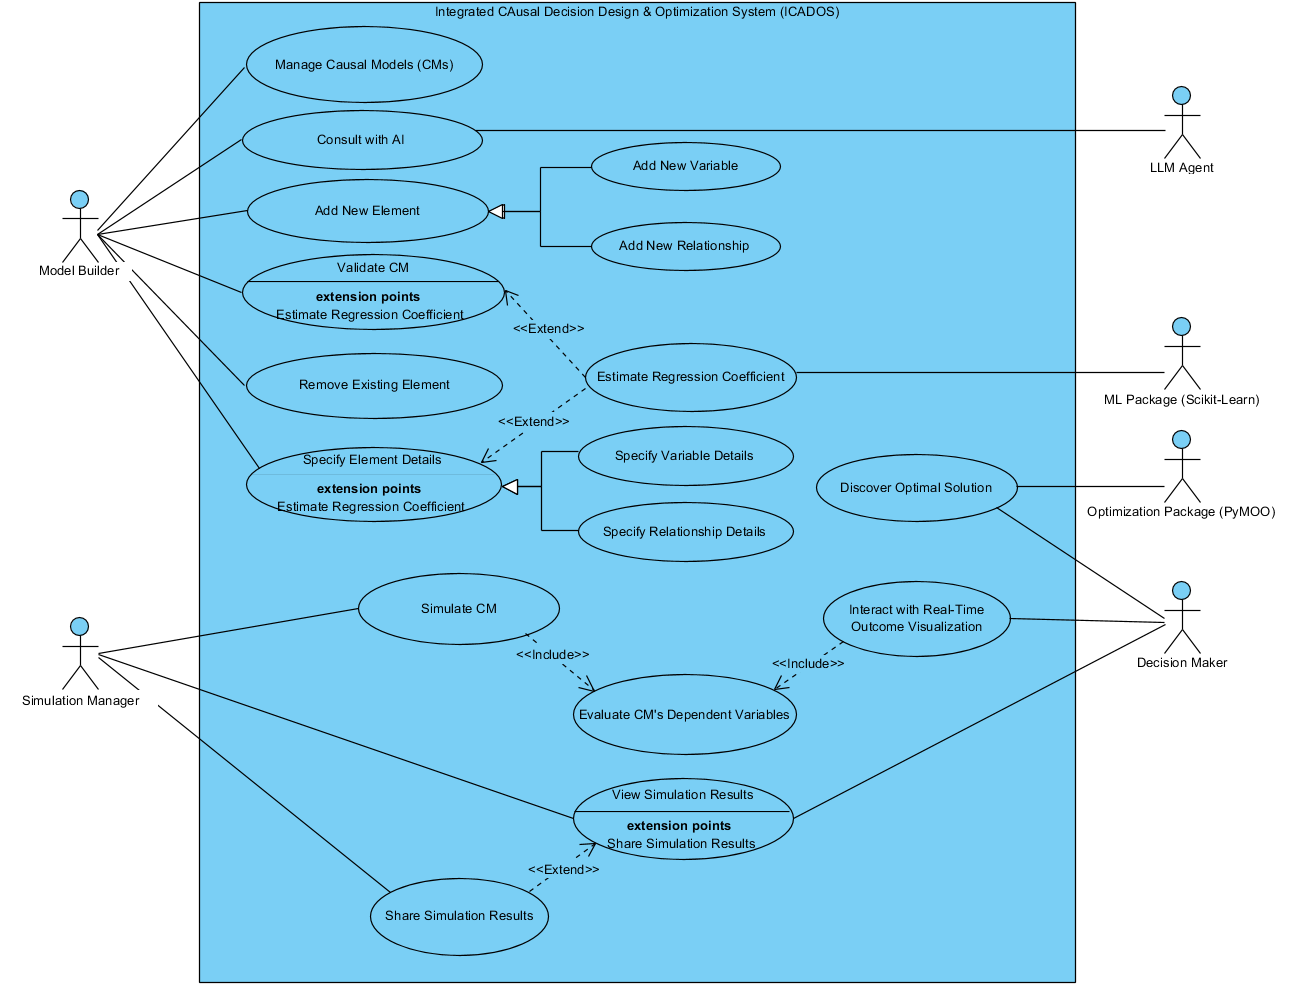
\includegraphics[width=6in]{Figures/ICADOS_UCD.png} % ≤ 6 inches wide
    \caption[ICADOS use-case diagram]{Use-case diagram for the main functional requirements of Integrated CAusal Decision Design and Optimization System (ICADOS)}
    \label{ICADOSUCD}
\end{figure}

\section{User Interface}
Since the mainstream operations that ICADOS performs are causal graph modeling, forward simulation, real-time visualization of the model outcomes, and optimization of the model's decision inputs, we have created a low-fidelity User Interface (UI) for each of these functions using JavaScript-based libraries including Data-Driven Documents (D3). Figure ~\ref{CDDInICADOS} illustrates the UI for building a causal model that a user with the \textit{Model Builder} role has access to. Once the user builds the causal network using the modeling tools on the left side of the canvas, they may click on the “Run Model” icon at the top middle of the screen. At this point, the system checks for the veracity of the model’s topology and logic (e.g., having an incoming or outgoing link for all the variables). If the model is verified, the system pops up an overlay modal as shown in Figure ~\ref{SIMModalICADOS} for specifying the model's computational assets such as mathematical functions or ML models to be assigned to each relationship.\par
\begin{figure}
    \centering
    % Ensure figure width fits within SFU margins
    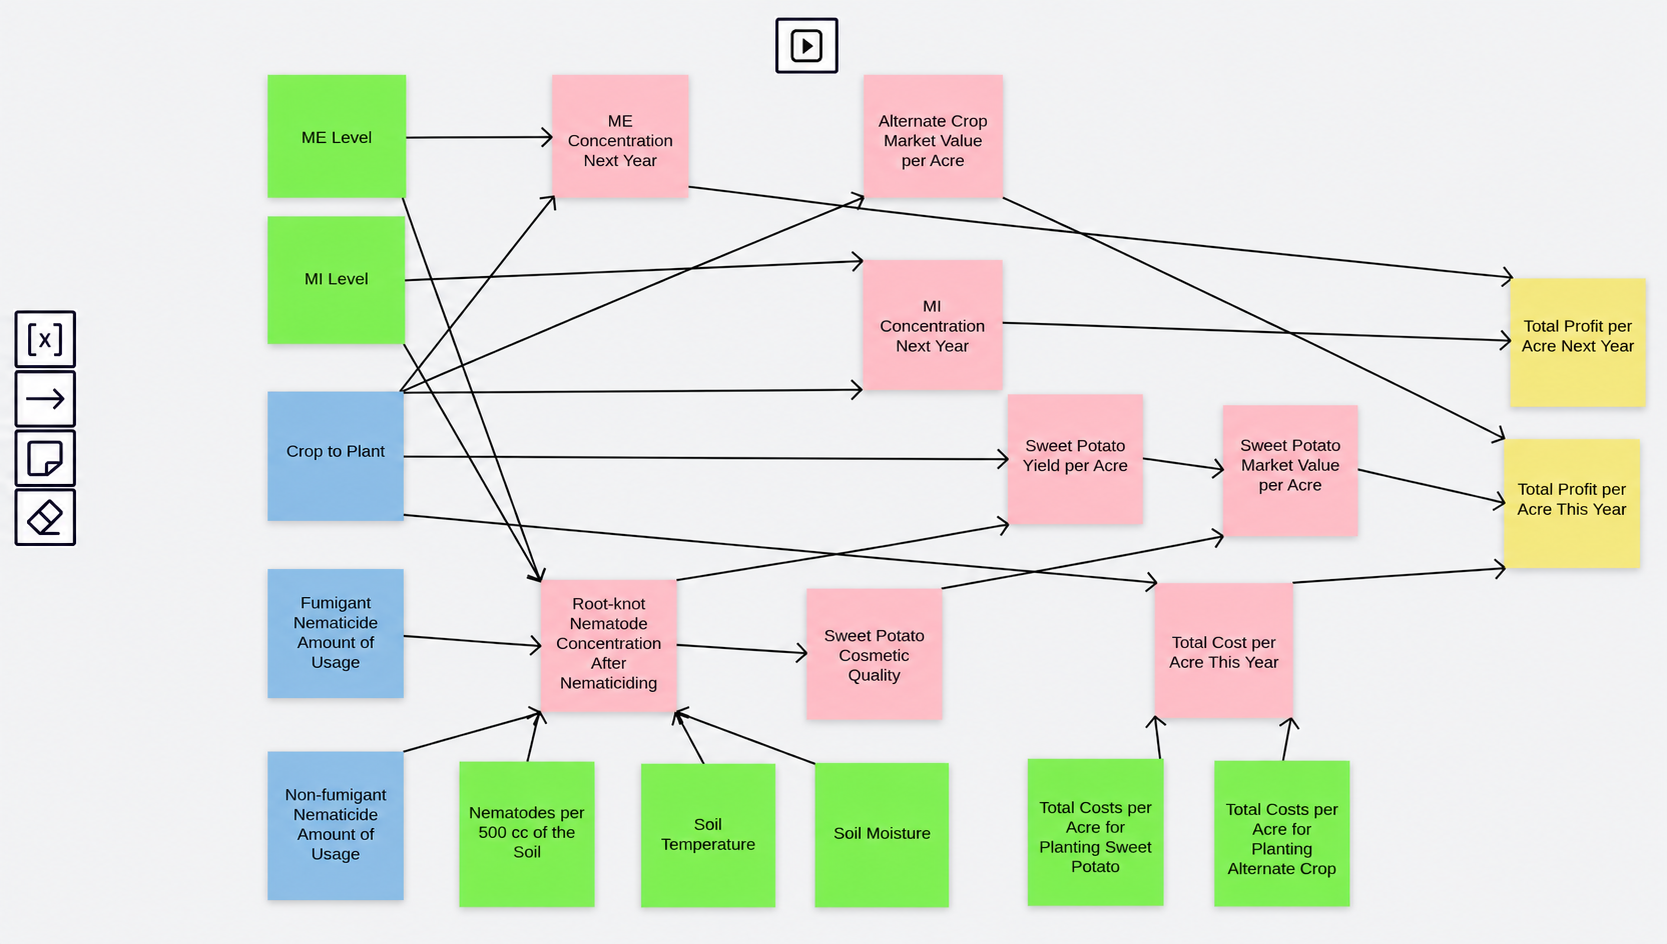
\includegraphics[width=6in]{Figures/CDDNematodesWithICADOS.png} % ≤ 6 inches wide
    \caption[ICODOS use-case diagram]{Causal decision diagram (CDD) in Figure ~\ref{CDDNematode}, rebuilt using ICADOS modeling environment. The interface enables users to assign a distinct background color to each variable category to facilitate visual differentiation. In the current configuration, decision variables are represented by blue nodes, external variables by green nodes, intermediate variables by pink nodes, and outcome variables by yellow nodes.}
    \label{CDDInICADOS}
\end{figure}
\begin{figure}
    \centering
    % Ensure figure width fits within SFU margins
    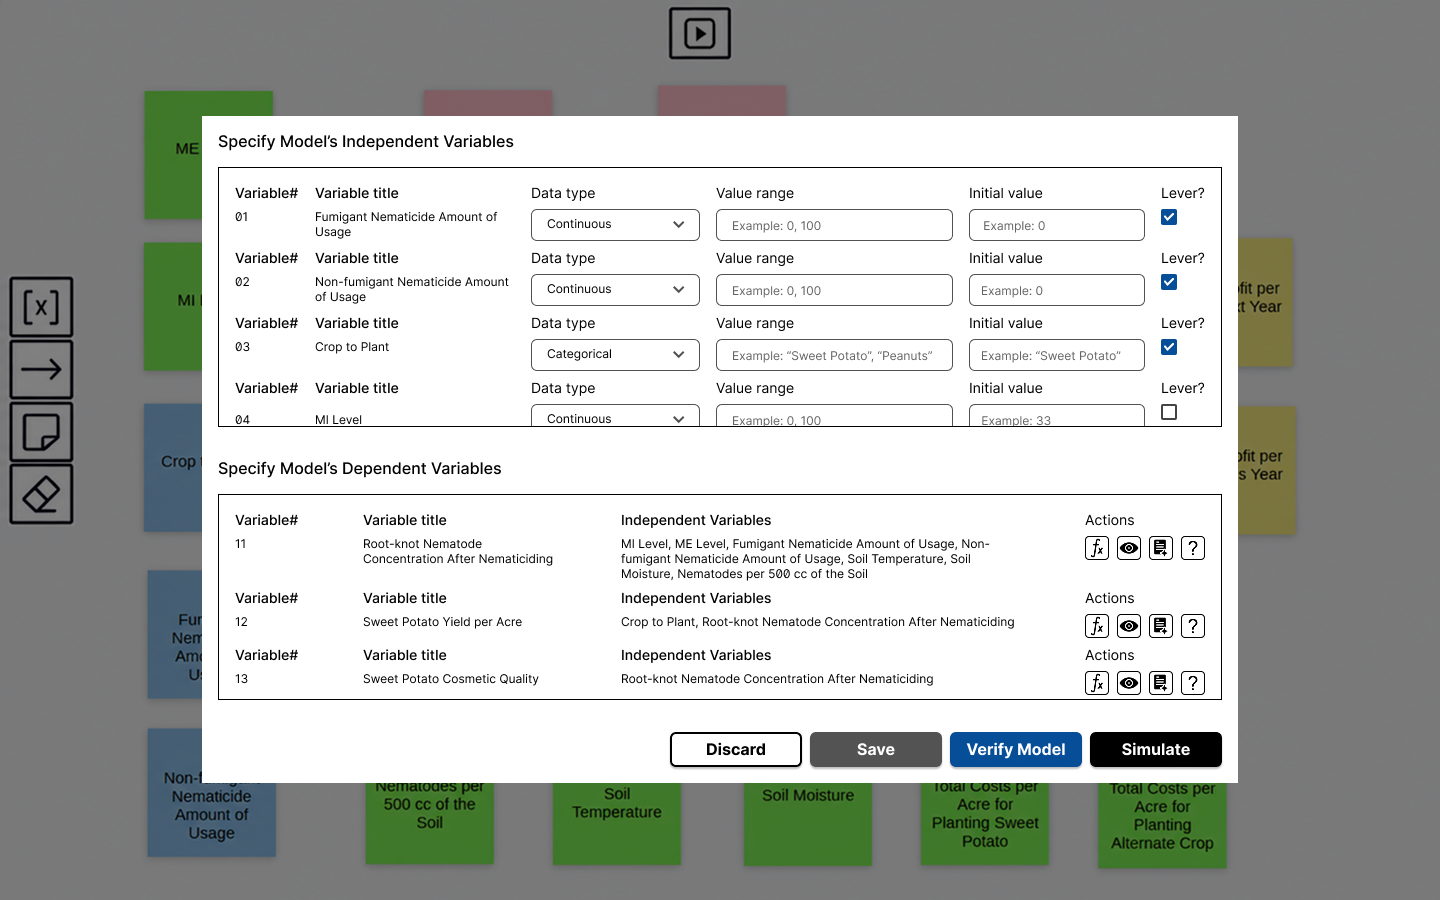
\includegraphics[width=6in]{Figures/ICADOS_SIMModal.png} % ≤ 6 inches wide
    \caption[ICADOS UI for specification of simulation data]{A modal in the ICADOS UI for specifying the simulation data for the CDD built in Figure~\ref{CDDInICADOS}}
    \label{SIMModalICADOS}
\end{figure}
The modal shown in Figure ~\ref{SIMModalICADOS} contains two sections. The top section of the modal is “Specify  Model's Independent Variables”, which contains a collective list of all lever and external variables for which users need to specify the data. In this section, users configure the information for these variables, including their \textit{Data type, Value range}, and \textit{Initial value}. For each variable listed in this section, Data Type can either be “Binary” to represent true/false decision space logic, “Continuous” that will make the corresponding variable get any real-number value in a specified range, or “Categorical” which will bind the range of values that the variable can get to those that are specified by the user in the "Value range" input field. The bottom section, “Specify Model's Dependent Variables”, is to prompt users to write an equation between each dependent Variable (Intermediates/Outcomes) and its independent variables. As seen in Figure ~\ref{SIMModalICADOS}, users can perform four different actions (visualized by icons) on every dependent variable listed in the bottom section of the modal. Clicking on the first icon from the left pops up a secondary modal prompting the user to enter a formula specifying the value of the selected dependent variable as a function of the corresponding independent variables. Illustrated in Figure ~\ref{FormulaWritingModalICADOS}, the formula writing modal contains an adjustable box for formula specification, as well as a "Resources" section from which users can select the computational resource of their interest (i.e., Variable, Function, and Operator) and add it to the formula box at the top. Once the user provides the formula in the box, they may save or discard the entered clauses and return to the main simulation setup interface. \par
\begin{figure}
    \centering
    % Ensure figure width fits within SFU margins
    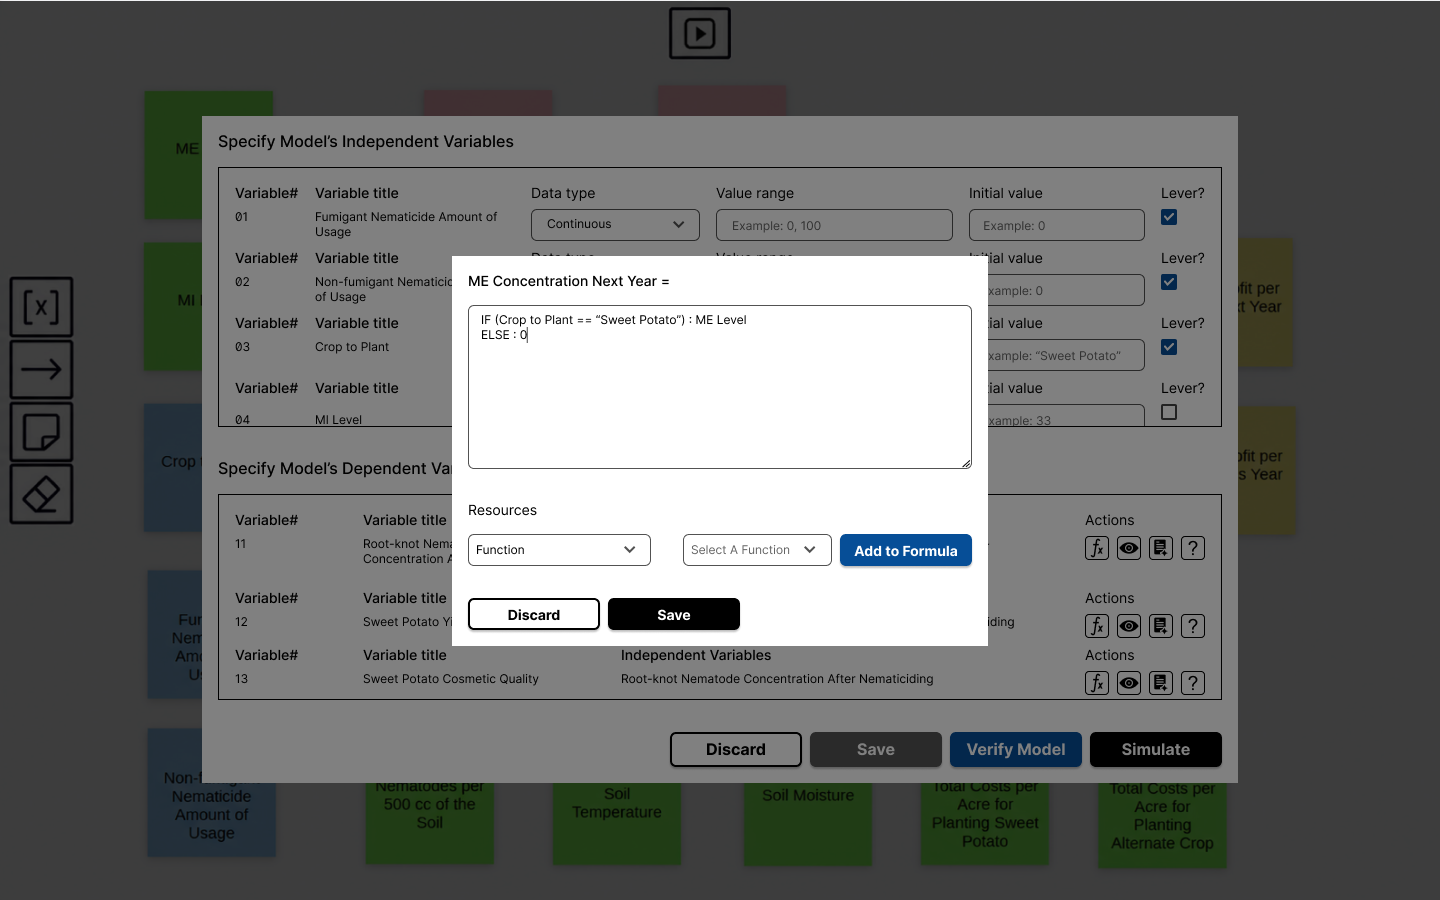
\includegraphics[width=6in]{Figures/ICADOS_FormulaWritingModal.png} % ≤ 6 inches wide
    \caption[ICADOS UI for formula writing]{A modal in the ICADOS UI for writing a formula to calculate the value of a variable (i.e., "ME Concentration Next Year") as a function of its independent variables (i.e., "Plant to Crop" and "ME Level")}
    \label{FormulaWritingModalICADOS}
\end{figure}
Clicking on the second icon opens up a modal in which users can view a graph visualizing the data points of the selected variable and one of its independent variables upon the user's choice. This feature is particularly useful when users seek to visually investigate whether the accessible data support an assumed causal relationship between two variables.

When the SCM is not explicitly known, users can employ the ICADOS' model learning capability to extract a structural function that relates the value of a dependent variable to those of its predictors. This is done by clicking on the third icon, which results in the modal illustrated in Figure ~\ref{ModelExtractionModalICADOS} appearing on the screen.\par
\begin{figure}
    \centering
    % Ensure figure width fits within SFU margins
    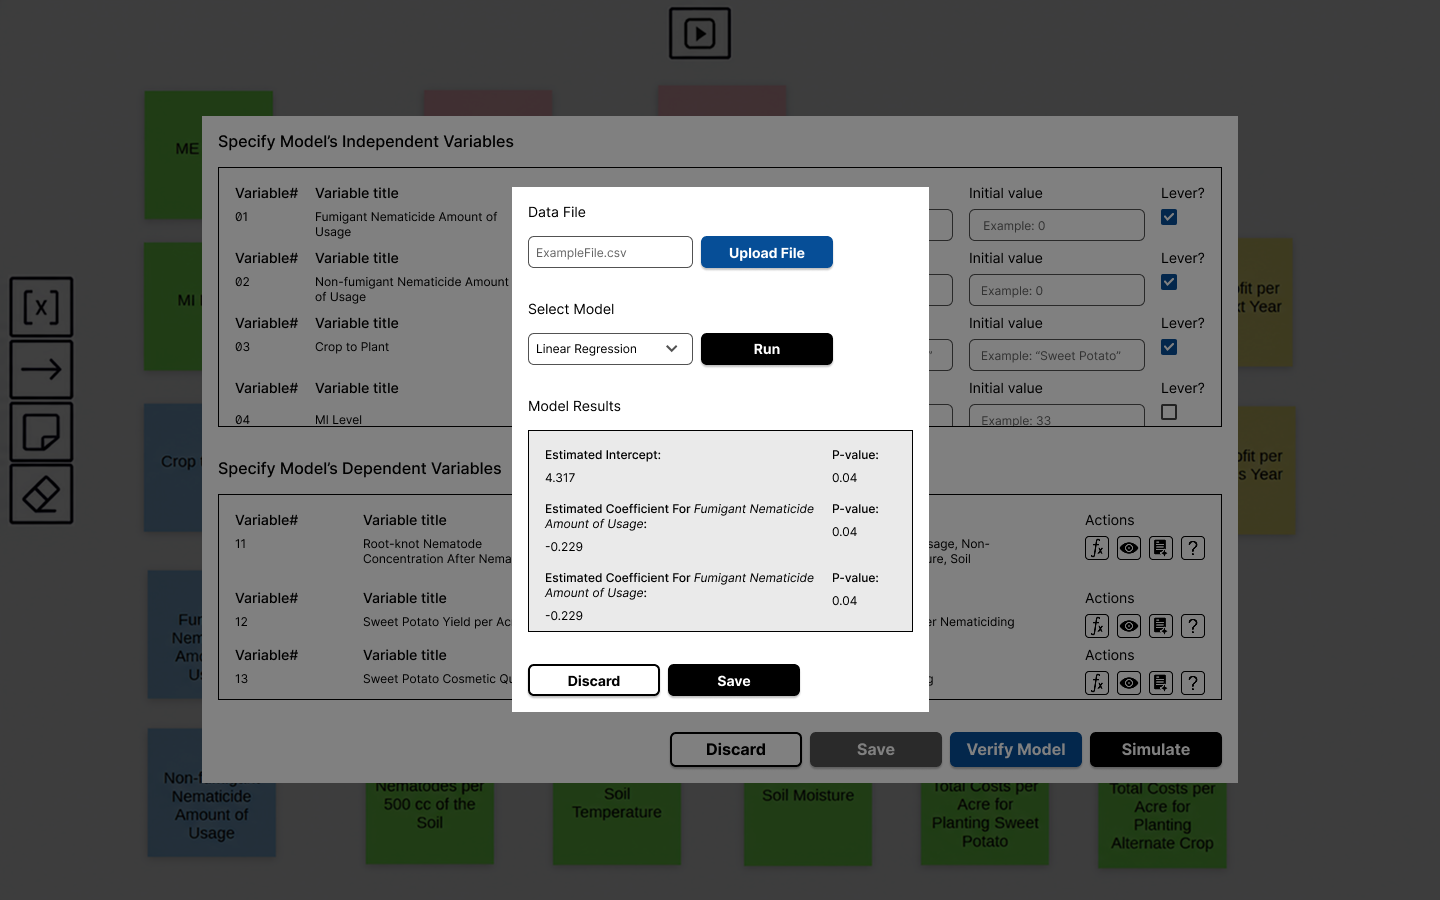
\includegraphics[width=6in]{Figures/ICADOS_ModelExtractionModal.png} % ≤ 6 inches wide
    \caption[ICADOS UI for model extraction]{A modal in the ICADOS UI for extracting a machine learning (ML) model to estimate the value of a dependent variable (i.e., "Root-knot Nematode Concentration After Nematiciding") as a function of its independent (parent) variables (e.g., "Fumigant Nematicide Amount of Usage").}
    \label{ModelExtractionModalICADOS}
\end{figure}
Users can use the file selector field at the top section of the modal shown in Figure ~\ref{ModelExtractionModalICADOS} to select a data file (in CSV format) containing the data of the dependent variable and its independent variables. After selecting the appropriate ML model (i.e., linear regression for continuous dependent variables) and hitting the "Run" button, the system computes all model parameters alongside their p-values and shows them inside the "Model Results" at the modal's bottom section. Users can save or discard the generated results and return to the main simulation modal screen.

The last action users can take on a dependent variable using the ICADOS simulation interface is the assignment of belief about the strength of causal relationships. Belief assignment is particularly essential for the later model verification process. To assign their beliefs about the strength of the relationships between the selected dependent variable and its independents, users click on the fourth icon, and the system opens the belief assignment modal. Illustrated in Figure ~\ref{BeliefAssignmentModalICADOS}, the modal only contains a table in which every row represents the causal relationship between the dependent variable and one of its independents. The user can select the level of his perceived causal strength for the corresponding relationship using the "perceived causal strength" field embedded in the row. The values of this field come in three levels as "1 (Weak)", "2 (Moderate)", and "3 (High)". Any change in the current values of the fields can be saved or discarded before returning to the main simulation screen.\par
\begin{figure}
    \centering
    % Ensure figure width fits within SFU margins
    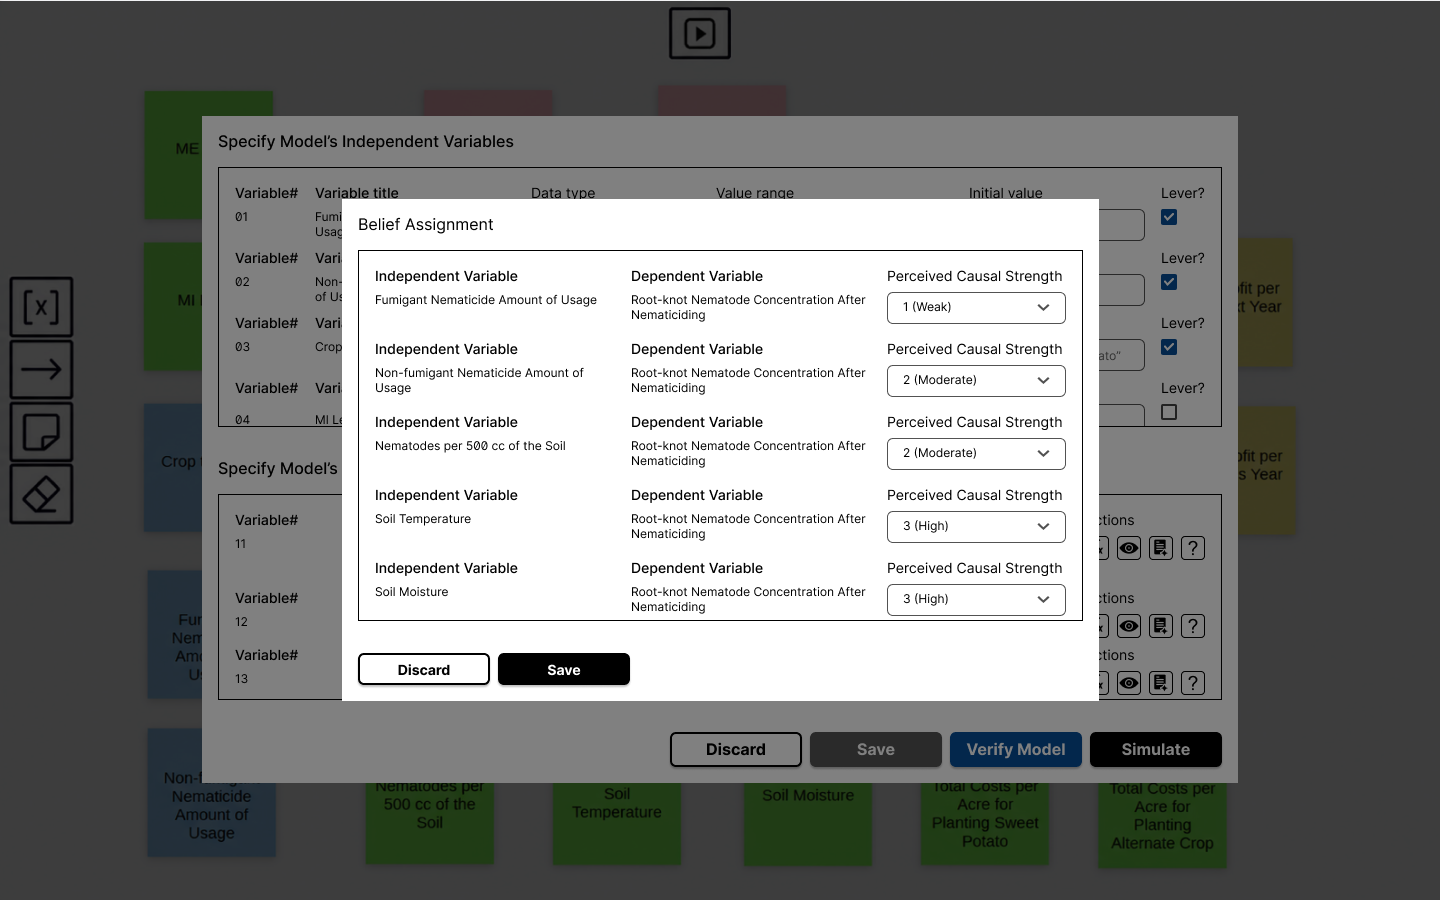
\includegraphics[width=6in]{Figures/ICADOS_BeliefAssignmentModal.png} % ≤ 6 inches wide
    \caption[ICADOS UI for causal belief assignment]{A modal in the ICADOS UI for specifying the user's level of confidence in the strength of the assumed causal relationships between a dependent variable (i.e., "Root-knot Nematode Concentration After Nematiciding") and its independent (parent) variables.}
    \label{BeliefAssignmentModalICADOS}
\end{figure}
Once the initial values and value ranges for the developed causal model's independent variables (i.e., levers and externals) and the structural functions for the model's dependent variables (i.e., intermediates and outcomes) are all specified, users can click on the “Simulate” button to run the forward simulation for calculating the values of the intermediates and outcomes. Before simulation, users can also click on the "Verify Model" button to have the entire causal graph verified. The model verification, however, can only be run if the user has previously assigned their perceived strength of all causal relationships inside every dependent variable's belief assignment modal shown in Figure ~\ref{BeliefAssignmentModalICADOS}. Finally, users can hit the "Save" button to save the configurations, or click on the "Discard" button to discard all configurations and move back to the elicitation and modeling canvas.

Upon successful completion of the simulation, the user interface transitions to the interactive visualization dashboard for solution exploration, as illustrated in Figure~\ref{OutcomeVIZICADOS}. At this stage, users assigned the \textit{Decision Maker} role can interact with user-controlled interface elements (e.g., sliders) to specify the values of decision and external variables while observing the corresponding simulated outcome values in real time. To accommodate diverse decision-making scenarios, the underlying visualization framework should support interactive, real-time visualizations for a variety of data types.

In the interactive dashboard shown in Figure~\ref{OutcomeVIZICADOS}, the "Levers" panel provides slider controls for specifying the values of continuous decision variables. In the illustrated example, the two sliders allow users to adjust the application rates of fumigant and non-fumigant nematicides within their respective feasible ranges, with the resulting changes in outcome variables being updated dynamically. In contrast, the value of the "Crop to Plant" variable is specified using a set of radio buttons, as this variable was previously defined as a categorical variable during the simulation configuration process.
\begin{figure}
    \centering
    % Ensure figure width fits within SFU margins
    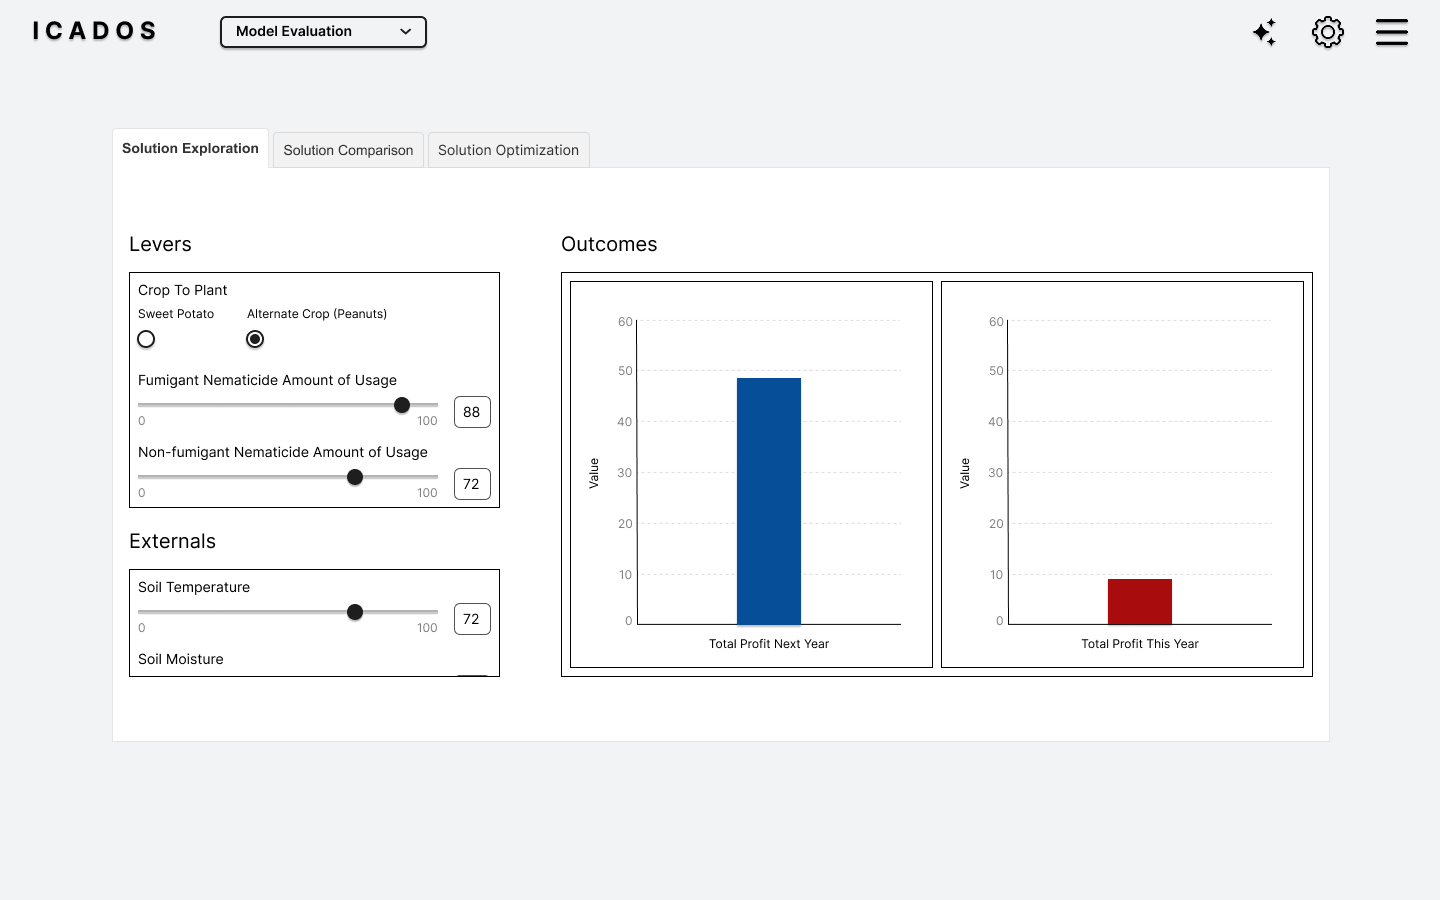
\includegraphics[width=6in]{Figures/OutcomeVIZ_ICADOS.png} % ≤ 6 inches wide
    \caption[ICADOS UI for real-time visualization of outcomes]{ICADOS UI for real-time visualization of simulated values for "Total Profit per Acre This Year" and "Total Profit per Acre Next Year" outcome variables. The values of the model's independent variables (e.g., levers and externals) are set by the user in the left panel using radio buttons and sliders, resulting in a real-time update of the model's dependent variables' values in the right.}
    \label{OutcomeVIZICADOS}
\end{figure}
As illustrated in Figure~\ref{OutcomeVIZICADOS}, the proposed "Model Evaluation" page comprises three functional tabs: "Solution Exploration", "Solution Comparison", and "Solution Optimization". Upon completion of the initial simulation, the "Solution Exploration" tab is displayed by default, allowing users to interactively examine the simulated outcomes under different decision scenarios. Users wishing to evaluate multiple scenarios simultaneously can navigate to the "Solution Comparison" tab, which provides functionality for the side-by-side comparison of outcomes across alternative decision scenarios. Alternatively, the "Solution Optimization" tab enables users to invoke the ICADOS computational engine to identify the most suitable solution from a set of candidate alternatives using a selected multi-criteria decision-making (MCDM) method.
 
\section{Technology Stack}
Even though the decision on what technologies to use for some undeveloped components of ICADOS has not yet been made, here we explain the technologies that have already been applied to develop the bits shown in the previous section. As capturing the perceived causal relationships between the contextual variables is considered the first main activity in our framework, we commenced the development phase by building a canvas-like environment (shown in Figure ~\ref{CDDInICADOS}) that system users can use to draw causal models (i.e., only CDD as of now) by adding variables (rectangles) and links (arrows). We have used HTML, CSS, and JavaScript with Scalable Vector Graphics (SVG) web components to build the essential stack for the modeling environment. After the user specifies and submits the initial variable values, functional relationships, and data models through the simulation configuration dialog, the corresponding information is serialized and transmitted to the simulation engine via its RESTful APIs. At the time of writing, these APIs have not yet been implemented and are therefore beyond the scope of the current prototype.

The simulation engine’s source code contains Python classes for each element of the causal model (including Variable, Equation, and the causal model itself) as well as methods and functions to fetch and operate on data or to compute values. As one of the expected functionalities of ICADOS is the ability of providing dataset and having the system train and generate the statistical model itself for a relationship in the model, the simulation engine makes use of multiple Python-source data science libraries such as NumPy, pandas, and scikit-learn to extract a mathematical function between a dependent variable and its independent variables inside the model. In Figure ~\ref{ICADOSSIMSource}, the code implementing the Python functions for extracting a linear regression model from a given dataset and computing CDD’s dependent variables (i.e., Intermediates and Outcomes) values has been illustrated. As shown in Figure ~\ref{ICADOSSIMSource}, the “ExtractModel” function gets a string argument for the dependent variable, a list of strings as independent variables, and a string for the data file’s title that is used to train the linear model. Once the model is trained and fitted, the function returns a list that contains regression coefficients for each independent variable in the linear regression model as well as the model’s intercept value as the last element in the returned list. The other function “ComputeCDDVars” computes the value of each dependent variable when the values of its independent variables are already computed. As a recursive function, it updates the list of uncomputed and computable variables in a given CDD after each computation step and passes it as an argument to itself until no uncomputed variable remains in the CDD.\par
\begin{figure}
    \centering
    % Ensure figure width fits within SFU margins
    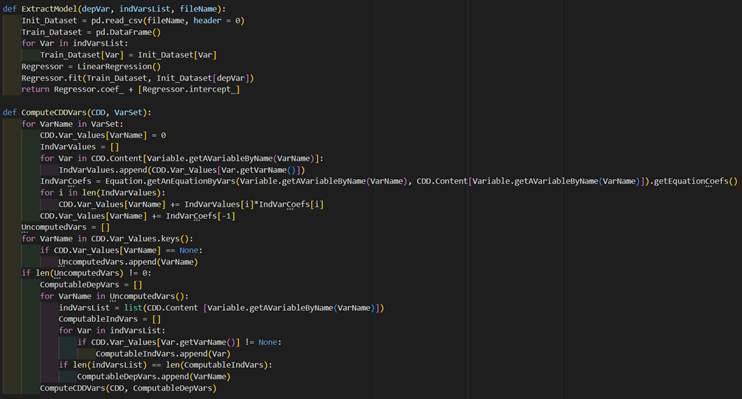
\includegraphics[width=6in]{Figures/ICADOS_SimFunction_Source.png} % ≤ 6 inches wide
    \caption[ICADOS source-code implementing the forward simulation of the values of a model's dependent variables]{ICADOS source-code implementing the forward simulation of the values of a model's dependent variables.}
    \label{ICADOSSIMSource}
\end{figure}
Once the simulation engine computes the values for intermediates and outcomes, it returns the list of computed values to the web client for generating visualization panels in Figure ~\ref{OutcomeVIZICADOS}. D3.js is particularly useful in this part for creating graphs, charts, and charts’ content (e.g., axes and bars). A client-server live connection is also established at this step to enable users to interact with the visualization tool in real-time using WebSocket connection protocols.

\chapter{Conclusion}
In this thesis, we were looking to extend the benefits of data-driven decision-making for organizational decision-makers by integrating multiple classes of data-driven tools and techniques with decision-makers’ knowledge of causal relationships inside the domain of purpose, as well as the provision of research-based guidelines for customization of these tools’ design and application according to cognitive capacities and other impactful humanistic properties of decision-makers. On this basis, in this final chapter, we summarize the strengths and novelties our work possesses, the limitations and weaknesses it faces, and how future research can address these limitations.
\section{Contribution}
We have contributed to the existing body of research in visual analytics and decision support systems in multiple aspects. The role of interactive data visualization in making informed decisions has not been formally studied beyond sense-making activities, as Dimara and Stasko~\cite{dimara_critical_2022} argued. Our proposed framework attempts to fill this gap by highlighting how data visualization—besides other DDTs—can assist DMs in activities beyond the Intelligence (i.e., sense-making) stage of the entire decision-making process, proposed by Simon~\cite{simon1960new}. By adopting a multidimensional approach, the orchestration and integration of different classes of tools other than VIZ (e.g., ML, SIM, etc.) for supporting the organizational decision-making process were formalized.\par
Another major contribution of this thesis pertains to the study of how data-driven technologies are or can be integrated based on human-centered guidelines, without necessarily omitting the role of task and data characteristics. In our framework, integration of multiple DDTs for a single activity in the decision-making process is preceded by the selection and customization of specific tools from every DDT class that has been found relevant for that activity (as a result of thematic analysis of DDDM literature in the 2nd chapter). Based on this, we highlighted many findings or recommendations from previous studies in three classes of task-relevant, data-relevant, and user-relevant, to be considered by DSS designers when they are selecting and customizing a specific tool from a parent DDT, or integrating the selected tools from the DDTs associated with the task of interest.\par
Furthermore, since the role of human decision-maker’s causal knowledge of the decision environment in selection of some actions for achieving desired outcomes has been mainly overlooked in DSS design studies, our framework provides an approach to integrate the visual models of human causal knowledge with DDTs (e.g., VIZ, ML, and TS) inside the Design phase of Simon’s model, for enhanced judgment of what outcomes are expected, upon taking a particular set of actions. This, in turn, increases the interpretability and justifiability of why DMs take some actions to address a decision problem.\par
Lastly, we introduced an integrated workflow for the discovery and selection of optimal solution(s) to a pre-modeled decision problem with the aid of interactive visualization (VIZ), mathematical optimization (MO), and simulation (SIM) techniques. Concerned with the reliability of a selected solution, a novel local sensitivity analysis (LSA) process workflow was formalized that is compatible with our human-centered approach. 
\section{Limitations}
Several limitations disallow the generalizability of the framework proposed in this work. The most notable challenge is related to the lack of a task-level integrated solution. Despite providing the logical workflow, we did not formally execute the process of selecting a tool from every associated DDT, customizing the selected tools, and integrating them for every task in different stages of Simon’s model, due to the existence of several data-level tasks and a large number of tools and design options for associated DDTs.\par
Another major weakness of our proposed framework pertains to the process of extracting recommendations (i.e.,\textit{rules}) from previous studies to guide the selection, customization, and integration of tools from every DDT. Unlike the process of tools discovery, which was executed systematically in the 2\textsuperscript{nd} chapter, we limited our recommendation discovery to only highlighting some recommendations in classical research publications, while they could have been derived by a systematic literature review to further enhance the task-level design and integration workflow.\par
\section{Future Works}
Being only elaborated at the conceptual and architectural level, the real-world impact of complying with our framework practices is not clear. In order to verify to what extent the application of a DSS that implements the integrative framework elevates the quality, efficiency, and subjective confidence of organizational decisions, a user study should be done on the improved version of the prototype system that was introduced in the 5\textsuperscript{th} chapter. Such a user study can employ a mixed-method approach to collect quantitative data regarding efficiency and accuracy, and qualitative data about how participants use the different features of the software to structure a decision problem and make a final decision. The insights from the qualitative data can then lead to another iteration for improving the DSS design, making it more usable and useful.\par
Furthermore, a series of studies is needed to address the limitations of the proposed framework, as explained in the previous section. The SCI (\textit{Selection, Customization}, and \textit{Integration}) workflow should be carefully executed for every data-level task (e.g., \textit{finding correlation, detecting anomalies}, etc.) that has been taxonomized in previous studies ~\cite{amar_low-level_2005,brehmer2013multi}. For instance, designing an integrated solution for finding correlation between data variables—a task that is aided by VIZ and TS—requires selecting the most suitable visualization structure (e.g., scatterplot) and correlation coefficient (e.g., \textit{Pearson}’s $r$), customizing the selected structure’s design (e.g., adjusting the ticks on the axes, or differentiating the plots’ color from the chart’s background), and integrating the calculated coefficient with the visualization structure (e.g., positioning the correlation coefficient value on top of the chart, or embedding it in an on-demand pop-up or tooltip view). Effective execution of this multidimensional SCI workflow is dependent on considering the research-based recommendations (i.e., \textit{user-relevant, task-relevant,} and \textit{data-relevant}), which should also be derived from a systematic literature review. Every integrated solution can later be set in the DSS as the default view for that particular data-level task when the user wants to perform it.\par
Another potential extension to the proposed framework is the inclusion of fuzzy data as the input values for both decision levers and externals. A given fuzzy set as the input of a variable can be representative of many things, including value uncertainty, time-series data, or assessments from multiple decision stakeholders. Providing fuzzy sets as the input of the levers will draw the employment of those optimization algorithms or MCDM tools that support fuzzy data (e.g., fuzzy-AHP).





%   BACK MATTER  %%%%%%%%%%%%%%%%%%%%%%%%%%%%%%%%%%%%%%%%%%%%%%%%%%%%%%%%%%%%%%
%
%   References and appendices. Appendices come after the bibliography and
%   should be in the order that they are referred to in the text.
%
%   If you include figures, etc. in an appendix, be sure to use
%
%       \caption[]{...}
%
%   to make sure they are not listed in the List of Figures.
%

\backmatter%
    \addtoToC{Bibliography}
    \bibliographystyle{plain}
    \bibliography{references}

\begin{appendices} % optional

\begin{landscape}
\thispagestyle{landscape-page}

\chapter{}
\vspace{-2em}
\small

\setlength{\LTcapwidth}{\linewidth}
\begin{longtable}{
p{5.5cm}
p{4cm}
p{6cm}
p{3.5cm}
}
\caption[]{Coding and classification of data-driven tools and techniques found across different papers in our collected set from the search in DDDM literature}
\label{A1:DDTSurvey}\\

\toprule
\textbf{Coded Method} &
\textbf{Involved Studies} &
\textbf{Intermediate Theme} &
\textbf{Final Theme} \\
\midrule
\endfirsthead

\multicolumn{4}{c}{\tablename\ \thetable\ (continued)}\\
\toprule
\textbf{Coded Method} &
\textbf{Involved Studies} &
\textbf{Intermediate Theme} &
\textbf{Final Theme} \\
\midrule
\endhead

\bottomrule
\endfoot

% =====================================================
% MACHINE LEARNING
% =====================================================

Linear Regression &
~\cite{Deng2017ScoliosisDSS}, ~\cite{Zhu2018EducationalDSS}, ~\cite{Monti2025RailwayBridgeDSS}, ~\cite{song2024building} &
\multirow{5}{6cm}{Conventional Supervised Machine Learning Methods} &
\multirow{19}{3.5cm}{Machine Learning (ML)} \\

Logistic Regression &
~\cite{VaughanHuxley2023PatientExtrication}, ~\cite{sreepathy2023design}, ~\cite{muller2021risk}, ~\cite{song2024building} &
& \\

Decision Tree &
~\cite{vandewiele2018decision}, ~\cite{feng2024adaptive}, ~\cite{Tarnowska2022TinnitusTherapy} &
& \\

K-nearest Neighbors (KNN) &
~\cite{Deng2017ScoliosisDSS} &
& \\

Support Vector Machine (SVM) &
~\cite{Deng2017ScoliosisDSS} &
& \\
\cline{1-3}

Rule-based Classification Method &
~\cite{Monti2025RailwayBridgeDSS}, ~\cite{Tarnowska2022TinnitusTherapy} &
Rule-based Machine Learning Methods &
\\
\cline{1-3}

Ad-hoc Classification Method &
~\cite{Zhu2018EducationalDSS}, ~\cite{Tarnowska2022TinnitusTherapy}, ~\cite{leem2023towards}, ~\cite{valdes2017clinical} &
Ad-hoc Machine Learning Methods &
\\
\cline{1-3}

Random Forest &
~\cite{Deng2017ScoliosisDSS}, ~\cite{ataei2024intelligent}, ~\cite{verboven2022treatment}, ~\cite{lee2024machine}, ~\cite{Tarnowska2022TinnitusTherapy} &
\multirow{2}{6cm}{Ensemble Machine Learning Methods} &
\\

(Extreme) Gradient Boosting &
~\cite{Kozielski2021LPGDSS}, ~\cite{makokha2025enhancing}, ~\cite{feng2024adaptive} &
&
\\
\cline{1-3}

Hidden Markov Model (HMM) &
~\cite{song2024building} &
\multirow{5}{6cm}{Unsupervised Machine Learning Methods} &
\\

K-means &
~\cite{Pahuja2024Dexter}, ~\cite{Milic2024DataCenterEnergy}, ~\cite{leem2023towards} &
&
\\

K-median &
~\cite{feng2024adaptive} &
&
\\

Association Rule Learning &
~\cite{Tarnowska2022TinnitusTherapy} &
&
\\

Gaussian Mixture Model (GMM) &
~\cite{cecconi2022data} &
&
\\
\cline{1-3}

Deep Neural Network (DNN) &
~\cite{Han2020WastewaterDecisionMaking}, ~\cite{miao2025research}, ~\cite{wang2023data}, ~\cite{kharazmi2018computer} &
\multirow{4}{6cm}{Neural Networks} &
\\

Recurrent Neural Network (RNN) &
~\cite{kim2025development} &
&
\\

Artificial Neural Network (ANN) &
~\cite{Chen2023TyphoonVolunteers} &
&
\\

Graph Neural Network (GNN) &
~\cite{li2024optimal}, ~\cite{price2025aura} &
&
\\
\cline{1-3}

Reinforcement Learning (RL) &
~\cite{krishnan2024data}, ~\cite{miao2025research}, ~\cite{wang2026intelligent} &
Reinforcement Learning Methods &
\\
\cline{1-4}

% =====================================================
% TRADITIONAL STATISTICS
% =====================================================

Autoregressive Integrated Moving Average (ARIMA) &
~\cite{krishnan2024data} &
Time-series Methods &
\multirow{2}{3.5cm}{Traditional Statistics (TS)}
\\
\cline{1-3}

Inferential Statistics Method &
~\cite{cavieres_methodology_2020}, ~\cite{Monti2025RailwayBridgeDSS}, ~\cite{muller2021risk}, ~\cite{sreepathy2023design}, ~\cite{ataei2024intelligent} &
Inferential Statistics Methods &
\\
\cline{1-4}
% =====================================================
% NATURAL LANGUAGE MODELS
% =====================================================

Natural Language Processing (NLP) &
~\cite{Shapa2021PoultryFarmers}, ~\cite{miao2025construction} &
Natural Language Processing &
\multirow{2}{3.5cm}{Natural Language Models (NLM)}
\\
\cline{1-3}

Large Language Model (LLM) &
~\cite{zhou2026safedrive} &
Large Language Models &
\\
\cline{1-4}
% =====================================================
% DATA VISUALIZATION
% =====================================================

Dashboard &
~\cite{Yang2010MacroeconomicDSS}, ~\cite{Han2020WastewaterDecisionMaking}, ~\cite{krishnan2024data}, ~\cite{DelaCal2026CulturalTourism}, ~\cite{Pahuja2024Dexter}, ~\cite{Dahl2022PathologyLaboratories}, ~\cite{Sheikhkhoshkar2025ConstructionDSS}, ~\cite{Osman2021SmartCities}, ~\cite{song2024building}, ~\cite{gaftandzhieva2023data}, ~\cite{kim2025development}, ~\cite{o20184d}, ~\cite{street2022data}, ~\cite{chorev2017data}, ~\cite{vandewiele2018decision}, ~\cite{sreepathy2023design}, ~\cite{peters2023data}, ~\cite{weiner_integrating_2015}, ~\cite{price2025aura}, ~\cite{lusher2014data}, ~\cite{hansotte2021supporting}, ~\cite{catalano2017using} &
Multi-view Data Visualization Structures &
\multirow{10}{3.5cm}{Data Visualization (VIZ)}
\\
\cline{1-3}

Line Chart &
~\cite{Yang2010MacroeconomicDSS}, ~\cite{Sonehara2019CyberPhysicalSociety}, ~\cite{Milic2024DataCenterEnergy}, ~\cite{RiosZertuche2020ElectronicDecisionSupport}, ~\cite{doderer2010sidekick} &
\multirow{6}{6cm}{Single-view Data Visualization Structures}
&
\\

Bar Chart &
~\cite{RiosZertuche2020ElectronicDecisionSupport} &
&
\\

Heatmap &
~\cite{muller2021risk} &
&
\\

Table &
~\cite{Yang2010MacroeconomicDSS}, ~\cite{RiosZertuche2020ElectronicDecisionSupport}, ~\cite{valdes2017clinical}, ~\cite{muller2021risk}, ~\cite{Tarnowska2022TinnitusTherapy}, ~\cite{Han2020WastewaterDecisionMaking}, ~\cite{ataei2024intelligent} &
&
\\

2D Map &
~\cite{Sonehara2019CyberPhysicalSociety} &
&
\\

3D Map &
~\cite{Ma2020EquipmentMaintenance} &
&
\\
\cline{1-3}

Causal Loop Diagram (CLD) &
~\cite{Hu2023MegaInfrastructure} &
\multirow{3}{6cm}{Specialized Data Visualization Structures}
&
\\

Stock-Flow Diagram (SFD) &
~\cite{Hu2023MegaInfrastructure} &
&
\\

Petri-net Model &
~\cite{ataei2024intelligent} &
&
\\
\cline{1-4}
% =====================================================
% MATHEMATICAL OPTIMIZATION
% =====================================================

Analytic Hierarchy Process (AHP) &
~\cite{Zhu2018EducationalDSS}, ~\cite{DelaCal2026CulturalTourism} &
\multirow{4}{6cm}{Conventional Multi-attribute Decision-making Methods}
&
\multirow{11}{3.5cm}{Mathematical Optimization (MO)}
\\

TOPSIS &
~\cite{Li2023UnbalancedBidding}, ~\cite{gaftandzhieva2023data} &
&
\\

Evidential Reasoning &
~\cite{fu2020data} &
&
\\

Weighted Scoring Method (WSM) &
~\cite{Yu2020FactorySimulation} &
&
\\
\cline{1-3}

Ad-hoc Multi-attribute Decision-making Method &
~\cite{amiri2024variant}, ~\cite{Monti2025RailwayBridgeDSS}, ~\cite{xue2022data} &
Ad-hoc Multi-attribute Decision-making Methods &
\\
\cline{1-3}
Improved Gene Expression Programming (IGEP) &
~\cite{zhang2021data} &
Conventional Multi-objective Optimization Methods &
\\
\cline{1-3}
Markov Decision Process (MDP) &
~\cite{svavza2024data} &
Stochastic Multi-objective Decision-making Methods &
\\
\cline{1-3}
Ad-hoc Multi-objective Optimization Method &
~\cite{Sheikhkhoshkar2025ConstructionDSS}, ~\cite{SalasMolina2018CashManagement}, ~\cite{miao2025research} &
Ad-hoc Multi-objective Optimization Methods &
\\
\cline{1-3}
Mixed-integer Programming (MIP) &
~\cite{tao2025data}, ~\cite{beykal2022data} &
Conventional Single-Objective Optimization Methods &
\\
\cline{1-3}
Ad-hoc Single-objective Optimization Method &
~\cite{feng2024adaptive}, ~\cite{wang2026intelligent} &
Ad-hoc Single-Objective Optimization Methods &
\\
\cline{1-3}
Fuzzy Multi-criteria Decision-making Method &
~\cite{gaftandzhieva2023data}, ~\cite{xue2022data} &
Fuzzy Multi-criteria Decision-making Methods &
\\
\cline{1-4}
% =====================================================
% SIMULATION
% =====================================================

Monte-Carlo Simulation (MCS) &
~\cite{Ma2020EquipmentMaintenance}, ~\cite{cecconi2022data} &
\multirow{2}{6cm}{Stochastic Simulation Methods}
&
\multirow{6}{3.5cm}{Simulation (SIM)}
\\

Multi-trial Scenario Simulation &
~\cite{ryan2014data} &
&
\\
\cline{1-3}
GNN-based Simulation &
~\cite{li2024optimal} &
\multirow{2}{6cm}{Data-driven Simulation}
&
\\

Single-trial Policy Outcome Simulation &
~\cite{chorev2017data} &
&
\\
\cline{1-3}
System Dynamic Simulation &
~\cite{Hu2023MegaInfrastructure}, ~\cite{kuhl2020data} &
Equation-based Simulation Methods &
\\
\cline{1-3}
Agent-based Simulation (ABS) &
~\cite{ElNouty2024LearningModel}, ~\cite{long2018data} &
Agent-based Simulation Methods &
\\
\end{longtable}
\end{landscape}

\end{appendices}
\end{document}